%-------------------------------------------------------------------------------
%                      Template Naskah Skripsi
%               	Berdasarkan format JTETI FT UGM
% 						(c) @gunturdputra 2014
%-------------------------------------------------------------------------------

%Template pembuatan naskah skripsi.
\documentclass{jtetiskripsi}

\renewcommand \thesection{\Alph{section}.}
\renewcommand \thesubsection{\arabic{subsection}.}

%Untuk prefiks pada daftar gambar dan tabel
\usepackage[titles]{tocloft}
\renewcommand\cftfigpresnum{Gambar\  }
\renewcommand\cfttabpresnum{Tabel\   }

%Untuk hyperlink dan table of content
\usepackage[hidelinks]{hyperref}
\newlength{\mylenf}
\settowidth{\mylenf}{\cftfigpresnum}
\setlength{\cftfignumwidth}{\dimexpr\mylenf+2em}
\setlength{\cfttabnumwidth}{\dimexpr\mylenf+2em}

% comment
\usepackage{comment}

%Untuk Bold Face pada Keterangan Gambar
\usepackage[labelfont=bf]{caption}

%Untuk caption dan subcaption
\usepackage{caption}
\usepackage{subcaption}
\usepackage{longtable}

\usepackage{draftwatermark}
\usepackage{tikz}
\SetWatermarkText{\centering{\tikz{\node[opacity=0.1]{
\includegraphics[width=0.8\paperwidth]{gambar/UNJ_LOGO.png}};}}}
\SetWatermarkAngle{0}
\SetWatermarkScale{1}

%pdf
\usepackage{pdfpages}

%table
\usepackage{graphics}

\usepackage{wrapfig}

%bibliography
\usepackage{natbib}

%equation
\usepackage{amsmath}
\usepackage{amssymb}
%algoritma
\usepackage{algorithm}
\usepackage{algpseudocode}


%listing
\usepackage{listings}


\usepackage{enumitem}



\definecolor{codegreen}{rgb}{0,0.6,0}
\definecolor{codegray}{rgb}{0.5,0.5,0.5}
\definecolor{codepurple}{rgb}{0.58,0,0.82}
\definecolor{backcolour}{rgb}{0.95,0.95,0.92}

\lstdefinestyle{mystyle}{
	backgroundcolor=\color{backcolour},   
	commentstyle=\color{codegreen},
	keywordstyle=\color{magenta},
	numberstyle=\tiny\color{codegray},
	stringstyle=\color{codepurple},
	basicstyle=\ttfamily\footnotesize,
	breakatwhitespace=false,         
	breaklines=true,                 
	captionpos=b,                    
	keepspaces=true,                 
	numbers=left,                    
	numbersep=5pt,                  
	showspaces=false,                
	showstringspaces=false,
	showtabs=false,                  
	tabsize=2
}

\lstset{style=mystyle}


%-----------------------------------------------------------------
%Disini awal masukan untuk data skripsi
%-----------------------------------------------------------------
\titleind{Perancangan \emph{User Interface Search Engine} Dengan Admin Console Untuk Manajemen dan Visualisasi Data Hasil Pengindeksan \texit{Search Engine}}

\fullname{Aldian Asmara}

\idnum{1313618032}

%\approvaldate{12 Februari 2019}
%\approvaldate{12 Februari 2019}

\degree{Sarjana Ilmu Komputer}

\yearsubmit{2024}

\program{Ilmu Komputer}

\dept{Ilmu Komputer}

\firstsupervisor{Muhammad Eka Suryana, M. Kom.}
\firstnip{198512232012121002}

\secondsupervisor{Med Irzal, M. Kom.}
\secondnip{197706152003121001}

%-----------------------------------------------------------------
%Disini akhir masukan untuk data proposal skripsi
%-----------------------------------------------------------------

\tolerance=1
\emergencystretch=\maxdimen
\hyphenpenalty=10000
\hbadness=10000

\begin{document}


\cover
%-----------------------------------------------------------------
%-----------------------------------------------------------------
%Disini akhir masukan untuk muka skripsi
%-----------------------------------------------------------------

\chapter*{\centering{\large{LEMBAR PERNYATAAN}}}

Saya menyatakan dengan sesungguhnya bahwa skripsi dengan judul 	\textbf{Perancangan \emph{User Interface Search Engine} dan Admin Console Untuk Manajemen dan Visualisasi Data Hasil Pengindeksan Search Engine}   yang disusun sebagai syarat untuk memperoleh gelar Sarjana komputer dari Program Studi Ilmu Komputer Universitas Negeri Jakarta adalah karya ilmiah saya dengan arahan dari dosen pembimbing.

Sumber informasi yang diperoleh dari penulis lain yang
telah dipublikasikan yang disebutkan dalam teks skripsi ini, telah dicantumkan dalam Daftar Pustaka sesuai dengan norma, kaidah dan etika penulisan ilmiah.

Jika di kemudian hari ditemukan sebagian besar skripsi ini bukan hasil karya saya sendiri dalam bagian-bagian tertentu, saya bersedia menerima sanksi pencabutan gelar akademik yang saya sanding dan sanksi-sanksi lainnya sesuai dengan peraturan perundang-undangan yang berlaku.

\vspace{.5cm}

\begin{tabular}{p{7.5cm}c}
	&Jakarta, 12 Januari 2024\\
	&\\
	&\\
	&\\
	&Aldian Asmara
\end{tabular}
\chapter*{\centering{\large{LEMBAR PERSEMBAHAN}}}

\null \vfill
\begin{flushright}
	\emph{Untuk Ibu, Bapak, Adik-Adik dan Diriku}
\end{flushright}

%\chapter*{\centering{\large{LEMBAR PENGESAHAN}}}

\begin{figure}[H]
	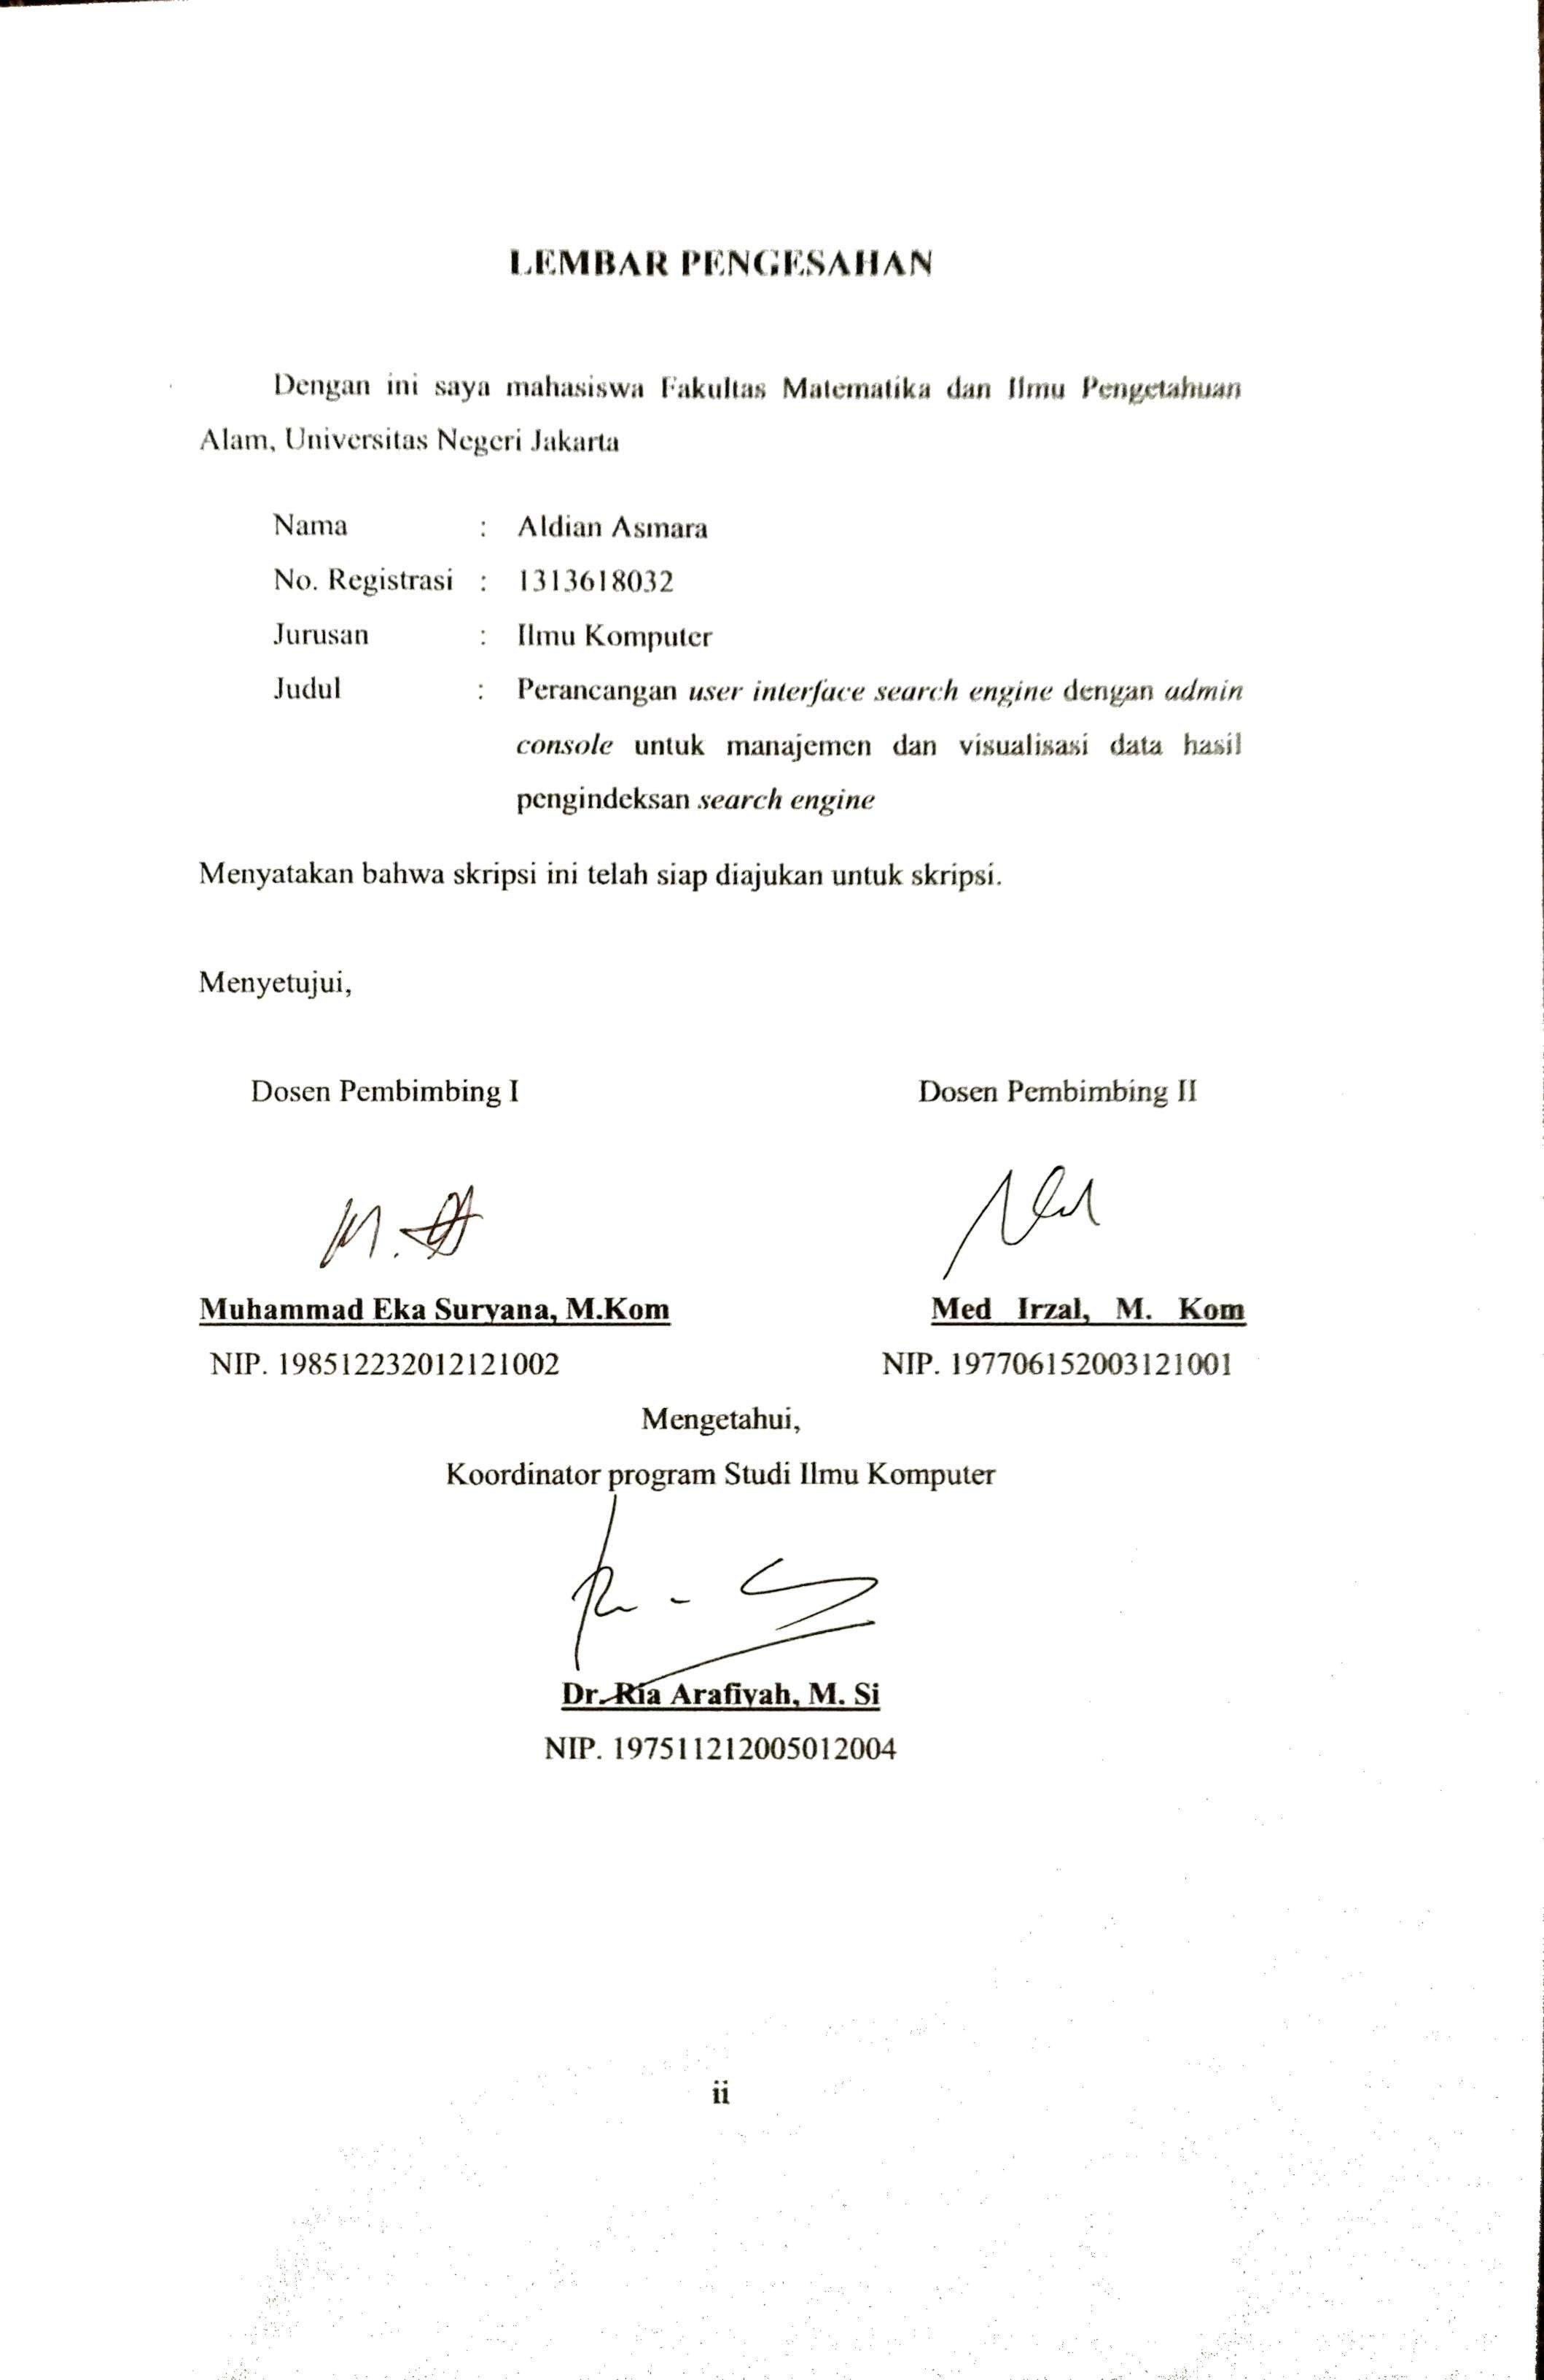
\includegraphics[scale=0.2]{gambar/lembar_pengesahan_skripsi}
\end{figure}
\chapter*{\centering \large KATA PENGANTAR}

Puji syukur penulis panjatkan ke hadirat Allah SWT, karena dengan rahmat dan karunia-Nya, penulis dapat menyelesaikan skripsi yang berjudul \textbf{"Perancangan \textit{User Interface Search Engine} dengan \textit{Admin Console} Untuk Manajemen dan Visualisasi Data Hasil Pengindeksan Search Engine"}. Keberhasilan dalam menyusun proposal skripsi ini tidak lepas dari bantuan berbagai pihak yang memberikan masukan guna sempurnanya proposal skripsi ini. Oleh karena itu, dengan kerendahan hati penulis mengucapkan banyak terima kasih kepada:

\begin{enumerate}
	
	\item{Yth. Para petinggi di lingkungan FMIPA Universitas Negeri Jakarta.}
	\item{Yth. Ibu Dr. Ria Arafiyah, M. Si selaku Koordinator Program Studi Ilmu Komputer.}
	\item{Yth. Bapak Muhammad Eka Suryana, M.Kom selaku Dosen Pembimbing I yang telah membimbing, mengarahkan, serta memberikan saran dan koreksi terhadap proposal skripsi ini.}
	\item{Yth. Bapak Med Irzal, M.Kom selaku Dosen Pembimbing II yang telah membimbing, mengarahkan, serta memberikan saran dan koreksi terhadap proposal skripsi ini.}
\end{enumerate}

Penulis menyadari bahwa penyusunan proposal skripsi ini masih jauh dari sempurna. Oleh karenanya, kritik dan saran yang bersifat membangun akan sangat membantu. Akhir kata, penulis berharap tugas akhir ini bermanfaat bagi semua pihak khususnya penulis sendiri.

\vspace{4cm}

\begin{tabular}{p{7.5cm}c}
	&Jakarta, 12 Januari 2024\\
	&\\
	&\\
	&\\
	&Aldian Asmara
\end{tabular}
\chapter*{\centering{\large{ABSTRAK}}}

\begin{spacing}{1}
	\textbf{ALDIAN ASMARA}. Perancangan \emph{User Interface Search Engine} dengan \textit{Admin Console} Untuk Manajemen dan Visualisasi Data Hasil Pengindeksan Search Engine. Skripsi. Fakultas Matematika dan Ilmu Pengetahuan Alam, Universitas Negeri Jakarta. 2024. Di bawah bimbingan Muhammad Eka Suryana, M.Kom dan Med Irzal, M.Kom.
	\newline
	\newline
	Mesin pencari merupakan sebuah program komputer yang berfungsi untuk membantu pengguna dalam menemukan informasi dengan kata kunci tertentu. Pada penelitian \citep{lazu} telah dirancang sebuah arsitektur \textit{search engine} dengan mengintegrasikan \textit{web crawler}, algoritma \textit{page ranking} dan \textit{document ranking}. Penelitian tersebut memiliki beberapa kekurangan yaitu tidak adanya \textit{admin console} untuk manajemen dan visualisasi data hasil pengindeksan \textit{search engine} yang telah dibuat. Penelitian ini memiliki tujuan untuk menyediakan suatu cara bagi pengguna untuk mengakses \textit{search engine} yang telah dibuat beserta \textit{admin console} untuk manajemen dan visualisasi data hasil pengindeksan \textit{search engine}. Informasi pendukung untuk melakukan penelitian ini berasal dari studi literatur jurnal-jurnal terkait dan diskusi yang diadakan peneliti dengan \textit{stakeholder}. Proses pengembangan yang digunakan dalam penelitian ini menggunakan metode \textit{Scrum} dengan menggunakan teknologi \textit{Python} dan \textit{Javascript}. Hasil akhir dari penelitian ini adalah sebuah  \textit{user interface} search engine \textit{admin panel} untuk manajemen dan visualisasi data hasil pengindeksan \textit{search engine} yang telah dibuat.
	\newline
	\newline
	\noindent \textbf{Kata kunci}:  \textit{search engine}, aplikasi, \textit{admin console}, \textit{scrum}
\end{spacing}


\chapter*{\centering{\large{ABSTRACT}}}

\begin{spacing}{1}
	\textbf{ALDIAN ASMARA}. \emph{Deisgning User Interface of a Search Engine with Admin Console for Managing and Visualizing Search Engine Indexing Result}. \emph{Thesis}. \emph{Faculty of Mathematics and Natural Sciences}, \emph{State University of Jakarta}. 2023. \emph{Supervised by} Muhammad Eka Suryana, M.Kom \emph{and} Med Irzal, M.Kom.
	\newline
	\newline
	\textit{The search engine is a computer program designed to assist users in finding information with specific keywords. In the research conducted by \citep{lazu}, an architecture for a search engine has been developed by integrating a web crawler, page ranking algorithm, and document ranking. The research has some shortcomings, such as the absence of an admin console for managing and visualizing of search engine's indexed data. The objective of this study is to provide a way for users to access the search engine along with an admin console for managing and visualizing the indexed data. Supporting information for this research is derived from literature studies of relevant journals and discussions held by researchers with stakeholders. The development process employed in this research follows the Scrum methodology, utilizing Python and Javascript technologies. The final result of this study is a user interface for the search engine admin panel to manage and visualize the indexed data in the created search engine. }
	\newline
	\newline
	\noindent \textbf{Keywords}: \textit{search engine}, \textit{application}, \textit{admin console}, \textit{scrum}
\end{spacing}


\begin{singlespacing}
\tableofcontents 
\addcontentsline{toc}{chapter}{DAFTAR ISI}
\listoffigures
\addcontentsline{toc}{chapter}{DAFTAR GAMBAR}
\listoftables
\addcontentsline{toc}{chapter}{DAFTAR TABEL}
\end{singlespacing}
\begin{counterpage}
\end{counterpage}
%Disini awal masukan untuk Bab
%-----------------------------------------------------------------
%!TEX root = ./template-skripsi.tex
%-------------------------------------------------------------------------------
% 								BAB I
% 							LATAR BELAKANG
%-------------------------------------------------------------------------------

\chapter{PENDAHULUAN}

\section{Latar Belakang Masalah}

Dengan bertambah banyaknya informasi yang berada di internet setiap harinya, tentu saja mencari informasi yang kita inginkan secara manual di \textit{Web} sangatlah memakan waktu. Oleh karena itulah \textit{search engine} atau mesin pencari hadir untuk menangani masalah tersebut. Mesin pencari atau search engine adalah program berbasis web yang dapat diakses di internet yang memiliki tujuan utama yaitu mencari yang informasi yang relevan dengan cepat terhadap \textit{query} yang pengguna kirim. Mesin pencari atau \textit{search engine} bekerja dengan cara mencocokan query dari pengguna kepada index yang search engine atau mesin pencari telah buat

Mesin pencari atau yang biasa disebut \emph{search engine} merupakan sebuah program komputer yang berguna untuk membantu pengguna dalam mencari situs web berdasarkan permintaan pencarian pengguna. Mesin pencari sebenarnya tidak berbeda dengan \textit{website} pada umumnya, hanya saja perannya lebih terfokus pada pengumpulan dan pengorganisasian berbagai informasi di internet sesuai dengan kebutuhan penggunanya. Selain untuk memudahkan pencarian, mesin pencari juga berguna untuk meningkatkan pengunjung sebuah situs web.

Kebanyakan \textit{search engine} atau mesin pencari yang ada di pasaran seperti Google, Bing dan Yahoo menyimpan aktivitas pengguna mereka dalam bentuk sebuah riwayat pencarian. Riwayat pencarian memberikan wawasan mengenai bagaimana suatu \textit{search engine} atau mesin pencari digunakan dan apa ketertarikan pengguna saat ini. Hal ini dibuat mungkin dikarenakan riwayat pencarian menyimpan apa saja yang pengguna cari pada \textit{search engine} atau mesin pencari dalam jangka waktu tertentu. Data riwayat pencarian ini dapat digunakan lebih jauh lagi untuk mengerti lebih dalam tentang pengguna.

Pada penelitian yang berjudul "Web Search Result Optimization by Mining the Search Engine Query Logs", sebuah metode diperkenalkan untuk mengoptimisasi hasil pencarian yang dimana metode yang diperkenalkan mempelajari dari riwayat pencarian dari penggunanya. Metode yang diperkenalkan ini memiliki tujuan untuk mengurangi waktu navigasi hasil pencarian oleh pengguna dengan cara memprediksi kebutuhan informasi dari pengguna. Metode yang diusulkan dari penelitian adalah klasterisasi query berdasarkan \textit{query} user dan \textit{feedback} user, kemudian halaman yang dikunjungi oleh user yang membentuk pola sequential dalam setiap \textit{cluster} dihasilkan dengan algoritma GSP (\textit{Generalized Sequential Patterns}). Tujuan akhirnya adalah melakukan perankingan kembali berdasarkan data sekuensial yang telah dihasilkan sebelumnya. Hasil dari penelitian yang dilakukan menunjukan hasil yang memuaskan dalam hal mengurangi ruang pencarian pengguna dan meningkatkan efektivitas search engine. Pendekatan yang dilakukan penelitian ini memerlukan setiap user memiliki perankingan dokumen yang berbeda dari user yang lain dikarenakan satu user dengan user lainnya pasti memiliki query pencarian dan tanggapan terhadap hasil pencarian yang berbeda juga \citep{improvingsearchresultbyminingusersquerylogs}.

Namun ada juga \textit{search engine} atau mesin pencari yang tidak menyimpan Riwayat pencarian penggunanya, seperti DuckDuckGo. DuckDuckGo merupakan \textit{search engine} atau mesin pencari yang memiliki tujuan agar penggunanya dapat menjelajah internet tanpa mengkhawatirkan data personal mereka dimanfaatkan oleh perusahaan lain. DuckDuckGo menjanjikan layanan pencarian yang privat, anonim dan menawarkan \textit{built-in tracker blocking} sehingga situs yang pengguna kunjungi akan kesulitan mengumpulkan informasi mengenai pengguna. DuckDuckGo menawarkan layanannya dalam \textit{platform} perangkat \textit{mobile} dan ekstensi \textit{desktop}. 

Visualisasi data adalah metode utama untuk membantu data mendapatkan interpretasi data dan juga menemukan nilainya. Data disajikan secara visual untuk menyampaikan interpretasi dasar mengenai apa yang data katakan tanpa adanya kesulitan \citep{datavisualizationbalogun}. Saat ini, visualisasi data atau visualisasi informasi menjadi topik yang menarik dan menjadi bidang penelitian yang luas. \citep{dbpediacasestudy} 

\iffalse
Graph adalah struktur matematika yang terdiri dari titik dan sisi yang menggambarkan hubungan antara beberapa entitas yang dimana titik memrepresentasikan entitas dan sisi yang ada di antara dua titik melambangkan bahwa dua entitas yang terhubung.\textit{Graph} dirumuskan dengan G=(V,E) yang terdiri dari beberapa titik \textit{vertices} (V) dan beberapa sisi \textit{edges} (pasangan titik). Banyak node dilambangkan dengan n = |V| dan banyaknya sisi dilambankgan dengan m = |E|. Apabila ada sisi yang menghubungkan antara titik i dengan titik j, dapat dilambangkan dengan notasi i -> j, jika graph tersebut tidak berarah maka dapat dilambangkan dengan notasi i <-> j (i dan j titik yang bertetangga). \citep{graphyifanhu}
\fi

Visualisasi grafik merupakan cara untuk menampilkan informasi yang terstruktur sebagai diagram dari grafik dan jaringan. \citep{graphvisualizationmeaning}. Visualisasi \textit{graph} dapat dilakukan dengan bantuan library open source diantaranya seperti GraphViz, D3.js, VivaGraph dan lain lain.\citep{graphyifanhu}

Dalam search engine, \textit{user interface} atau tampilan merupakan hal yang penting mengingat \textit{search engine} sering sekali digunakan dalam kehidupan sehari-hari bahkan menjadi bagian hidup dari seseorang. Menurut \citep{alonsoumarbaezaricardo}, pada umumnya, skenario dari penggunaan \textit{user interface} atau tampilan dari \textit{search engine} adalah sebagai berikut: 

\begin{enumerate}
	\item Pengguna memiliki kata yang ingin dicari dan mengirimkannya kepada mesin pencari atau \textit{search engine}
	\item  \textit{Search engine} merespon kata yang dikirimkan oleh user
	\item \textit{Search engine} akan mencari dokumen yang sesuai dengan query yang pengguna kirim dan menampilkannya ke tampilan \textit{search engine}
	\item Yang terakhir user menentukan apakah dokumen yang diterima user relevan atau tidak dengan yang diharapkan pengguna
\end{enumerate}

%Pengguna memiliki kata yang ingin dicari dan mengirimkannya kepada mesin pencari atau \textit{search engine} (1). \textit{Search engine} merespon kata yang dikirimkan oleh user (2). \textit{Search engine} akan mencari dokumen yang sesuai dengan query yang pengguna kirim dan menampilkannya ke tampilan \textit{search engine} (3). Yang terakhir user menentukan apakah dokumen yang diterima user relevan atau tidak dengan yang diharapkan pengguna (4).

Pada penelitian "Perancangan arsitektur \textit{search engine} dengan mengintegrasikan \textit{web crawler}, algoritma \textit{page ranking}, dan \textit{document ranking}" \citep{lazu} telah dirancang arsitektur \textit{serch engine} berbasis \textit{console}. Pada penelitian ini terdapat beberapa kekurangan yaitu tidak adanya \textit{admin console} untuk manajemen dan visualisasi data hasil pengindeksan \textit{search engine} yang telah dibuat.

Penelitian ini akan merancang tampilan dari \textit{search engine} dengan \textit{admin console} untuk visualisasi dan manajemen hasil indeks dengan mengintegrasikan penelitian dari \cite{lazu} yang berfokus pada perancangan arsitektur \textit{search engine} dengan mengintegrasikan \textit{web crawler}, algoritma \textit{page ranking} dan \textit{document ranking}.

\section{Rumusan Masalah}
Dari uraian latar belakang di atas, perumusan masalah pada penelitian ini adalah “Bagaimana perancangan \textit{user interface} \textit{search engine} dengan \textit{admin console} untuk manajemen dan visualisasi data hasil pengindeksan \textit{search engine}”.

\section{Pembatasan Masalah}
Pembatasan masalah pada penelitian ini antara lain:
\begin{enumerate}
	\item Penelitian ini menggunakan \textit{search engine} yang telah dibuat oleh \cite{lazu}.
	\item Rancangan tampilan yang akan dibuat hanya berfokus untuk tampilan \textit{desktop}.
\end{enumerate}

\section{Tujuan Penelitian}
Membuat \textit{user interface} dari \textit{search engine} dengan \textit{admin console} yang telah dibuat pada penelitian \cite{lazu}

\section{Manfaat Penelitian}
\begin{enumerate}
%	\item Bagi penulis
%	
%	Memperluas pengetahuan tentang \textit{search engine} dan memperoleh gelar sarjana di bidang Ilmu Komputer, serta menjadi media untuk penulis dalam mengaplikasikan ilmu yang didapatkan dari kampus.
	
	\item Bagi Program Studi Ilmu Komputer
	
	Penelitian ini dapat menjadi pembuka untuk penelitian di masa depan, dan dapat memberikan panduan bagi mahasiswa program studi Ilmu Komputer tentang rancang bangun aplikasi \textit{search engine}.
	
%	\item Bagi Universitas Negeri Jakarta
%	
%	Menjadi evaluasi akademik program studi Ilmu Komputer dalam penyusunan skripsi sehingga dapat meningkatkan kualitas pendidikan dan lulusan program studi Ilmu Komputer di Universitas Negeri Jakarta.
	
\end{enumerate}



% Baris ini digunakan untuk membantu dalam melakukan sitasi
% Karena diapit dengan comment, maka baris ini akan diabaikan
% oleh compiler LaTeX.
\begin{comment}
\bibliography{daftar-pustaka}
\end{comment}

 %!TEX root = ./template-skripsi.tex
%-------------------------------------------------------------------------------
%                            BAB II
%               KAJIAN TEORI
%-------------------------------------------------------------------------------

\chapter{KAJIAN PUSTAKA} 

\section{\textit{Search Engine}}
\textit{Search Engine} merupakan sebuah perangkat lunak yang dirancang untuk mencari informasi dalam \textit{internet}. Dalam penggunaannya, pengguna memasukan kata kunci yang ingin pengguna cari dalam \textit{search engine} dan \textit{search engine} akan menampilkan daftar dokumen, suara, gambar, \textit{video} dan lain lain yang relevan dengan kata kunci yang pengguna masukkan.

\textit{Search engine} menggunakan sebuah perangkat lunak bernama \textit{crawler} yang bertugas untuk memindai dan meng-\textit{index} halaman \textit{web} yang berada di \textit{internet}. \textit{Crawler} ini mengikuti tautan dari satu halaman ke halaman lainnya mengumpulkan informasi mengenai konten dan struktur \textit{website}. Data yang berhasil dikumpulkan tersebut lalu disimpan dalam sebuah \textit{database} yang membentuk \textit{search engine} index. Beberapa contoh \textit{search engine} yang populer pada saat ini adalah Google, Yahoo, Bing, Baidu dan Yandex.


\section{\textit{Agile}}
Pengembangan perangkat lunak menggunakan \textit{agile} merupakan salah satu metode pengembangan perangkat lunak yang ada. Kata "\textit{agile}" memiliki arti cepat, ringan dan bebas bergerak. Konsep pengembangan perangkat lunak menggunakan \textit{agile} ditemukan oleh Kent Beck dan 16 koleganya dengan menyatakan \textit{agile} adalah cara dalam membangun sebuah perangkat lunak dengan cara mengerjakannya dan membantu satu sama lain dalam membangunnya dalam satu waktu. Dalam pengembangan perangkat lunak menggunakan \textit{agile}, interaksi dan personil adalah hal yang penting dibandingkan proses dan alat kerja, Perangkat lunak yang bekerja lebih pentung dari dokumentasi yang lengkap, Kolaborasi antara klien lebih penting dari negosiasi kontrak dan responsif dalam perubahan adalah hal yang lebih penting dari mengikuti rencana yang telah dibuat. Spertim model lainnya, \textit{agile} memiliki kelebihan dan tidak cocok untuk semua tipe projek. \textit{Agile} membuat model proses yang toleran terhadap perubahan kebutuhan sehingga perubahan dapat dilakukan dengan cepat \citep{scrum}.

\section{\textit{Scrum}}
\textit{Scrum} dikembangkan oleh Jeff Sutherland di tahun 1993 dan memiliki tujuan untuk menjadi metode pengembangan dan manajemen yang mematuhi prinsip \textit{Agile}. Fokus dalam metode ini adalah "strategi, sebuah metode pengembangan perangkat lunak holistik yang fleksibel dimana tim pengembang bekerja sebagai satu unit untuk mencapai tujuan utama yang sama". 

Dalam pelaksanaannya, \textit{scrum} menjadi tiga bagian yaitu \textit{Product Owner}, \textit{Scrum Master} dan \textit{Team}. \textit{Product Owner} merupakan seseorang yang bertanggung jawab untuk menentukan spesifikasi atau perangkat lunak yang ingin dibangun. \textit{Product Owner} akan membuat kebutuhan yang akan diselesaikan oleh tim atau lebih dikenal sebagai \textit{Product Backlog}. \textit{Team} merupakan suatu entitas yang mengerjakan projek seperti analis bisnis, sistem analis, pengembang, penguji dan lain lain. \textit{Team} merupakan entitas yang bertanggung jawab dalam menyelesaikan \textit{Product Backlog} yang telah disediakan oleh \textit{Product Owner}, yang dimana setiap anggota dari \textit{Team} bertanggung jawab dalam setiap tugas dalam \textit{Product Backlog} yang telah dibagikan. \textit{Scrum Master} adalah seseorang yang akan memperkenalkan dan mengimplementasikan bagaiman \textit{Scrum} bekerja pada \textit{Team} dan memastikan semua orang dalam projek mengimplementasikan metode \textit{Scrum} \citep{scrum}.

Pengerjaan projek dengan metode \textit{Scrum} dimulai dengan penggambaran bagaimana sistem yang akan dibuat. Selanjutnya, \textit{Project Owner} menggambarkan proses bisnis atau rencara kedalam \textit{Product Backlog}. \textit{Product Backlog} merupakan sekumpulan rencana yang harus diselesaikan oleh \textit{Team}. Terdapat sebuah \textit{sprint} dalam metode \textit{scrum}. \textit{Sprint} merupakan tujuan yang ingin dicapai dalam \textit{sprint} selanjutnya. Setiap \textit{sprint} dibulai dengan \textit{Sprint Meeting Planning} yang merupakan aktivitas untuk menentukan \textit{sprint} apa yang akan dilakukan pada \textit{sprint} dilakukan selanjutnya. Setiap harinya, setiap anggota \textit{Team} berkumpul dan berdiskusi mengenai apa yang telah dilakukan setelah \textit{Daily Scrum Meeting} sebelumnya, masalah apa yang dihadapi, dan apa yang akan dikerjakan selanjutnya. Pertemuan ini direncanakan oleh \textit{Scrum Master} dan setiap penghujung \textit{sprint} akan dilakukan pertemuan untuk mendemonstrasikan apa saja yang telah dikerjakan \citep{scrum}.


\begin{figure}[H]
	\centering
	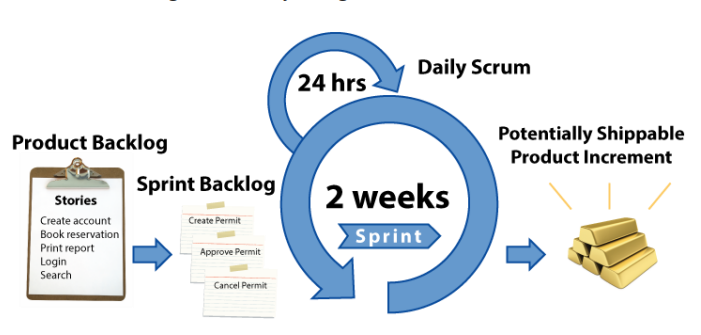
\includegraphics[keepaspectratio, width=12cm]{gambar/scrum-flow}
	\caption{Alur kerja scrum}
	\label{gambar:scrum-flow.png}
\end{figure}


\section{Perancangan \textit{User Interface}}

\textit{User Interface} adalah ilmu tentang tata letak grafis suatu web atau aplikasi \citep{userinterface1}. Cakupan \textit{User Interface} adalah tombol yang akan diklik oleh pengguna, teks, gambar, text entry fields, dan semua item yang berinteraksi dengan pengguna. Termasuk layout, animasi, transisi, dan semua interaksi kecil. UI mendesain semua elemen visual, bagaimana pengguna berinteraksi dengan halaman web dan apa yang ditampilkan di halaman web. Elemen visual yang ditangani oleh seorang desainer UI adalah skema warna, menentukan bentuk tombol, serta menentukan jenis font yang digunakan untuk teks. Desainer UI harus bisa membuat tampilan bagus yang akan meningkatkan kesetiaan pengguna. 
\subsection{Layout dan Spacing}
\textit{White spacing} merupakan jarak yang diberikan antara dua komponen baik itu jarak horizontal maupun vertikal. \textit{White spacing} diperlukan untuk memberikan setiap komponen ruang untuk bernafas. Dalam membuat \textit{white spacing} ada beberapa pendekatan diantaranya adalah pemberian \textit{white space} secara \textit{incremental} dari ukuran kecil hingga ke ukuran yang lebih besar. Pendekatan ini hanya meraih ukuran \textit{white spacing} minimum untuk terlihat bagus dan pada dasarnya dalam tampilan yang baik biasanya diperlukan lebih banyak white spacing. Pendeketan yang lebih baik dalam perancangan \textit{white spacing} yang baik adalah dengan mula mula memberikan komponen nilai \textit{white spacing} yang besar, dan lakukan pengurangan nilai \textit{white spacing} sampai pengguna merasa puas dengan nilai \textit{white spacing} yang diberikan. 

\begin{figure}[H]
	\centering
	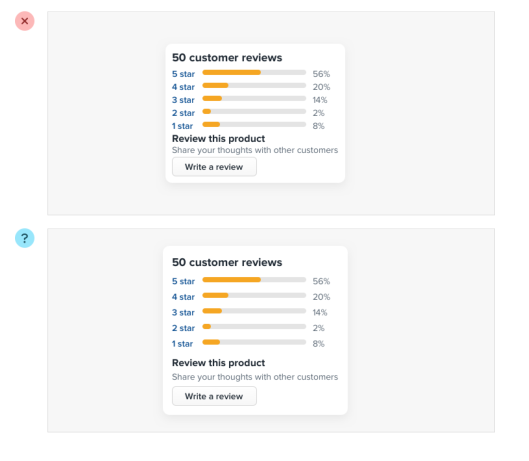
\includegraphics[keepaspectratio, width=12cm]{gambar/refactoring-ui-g1.png}
	\caption{Penentuan \textit{white spacing} dengan cara \textit{decremental} \citep{refactoringui}}
	\label{gambar:refactoring-ui-g1.png}
\end{figure}

Pada dasarnya komponen yang mempunyai banyak ruang untuk istirahat atau \textit{white spacing} terlihat lebih bersih dan simpel, namun ada beberapa kasus dimana \textit{white spacing} yang sedikit dan rapat dapat digunakan. Sebagai contoh, dalam perancangan tampilan \textit{dashboard}, yang dimana dalam tampilan \textit{dashboard} diperlukan untuk memuat informasi dalam jumlah banyak yang memungkinkan informasi tersebut terlihat dalam satu halaman.

\begin{figure}[H]
	\centering
	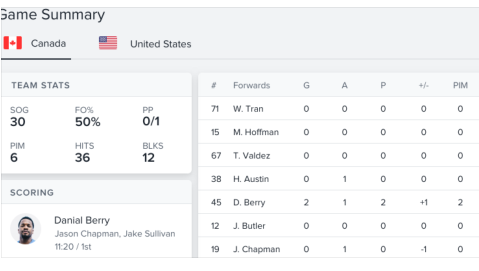
\includegraphics[keepaspectratio, width=12cm]{gambar/refactoring-ui-g2.png}
	\caption{Tampilan dashboard dengan nilai \emph{white spacing} yang kecil \citep{refactoringui}}
	\label{gambar:refactoring-ui-g2.png}
\end{figure}

Dalam mendesain sebuah \textit{layout} tidaklah harus mengisi seluruh \textit{white space} yang ada. Mengisi seluruh \textit{white space} yang ada hanya akan membuat tampilan lebih sulit untuk diinterpretasikan oleh pengguna.

\begin{figure}[H]
	\centering
	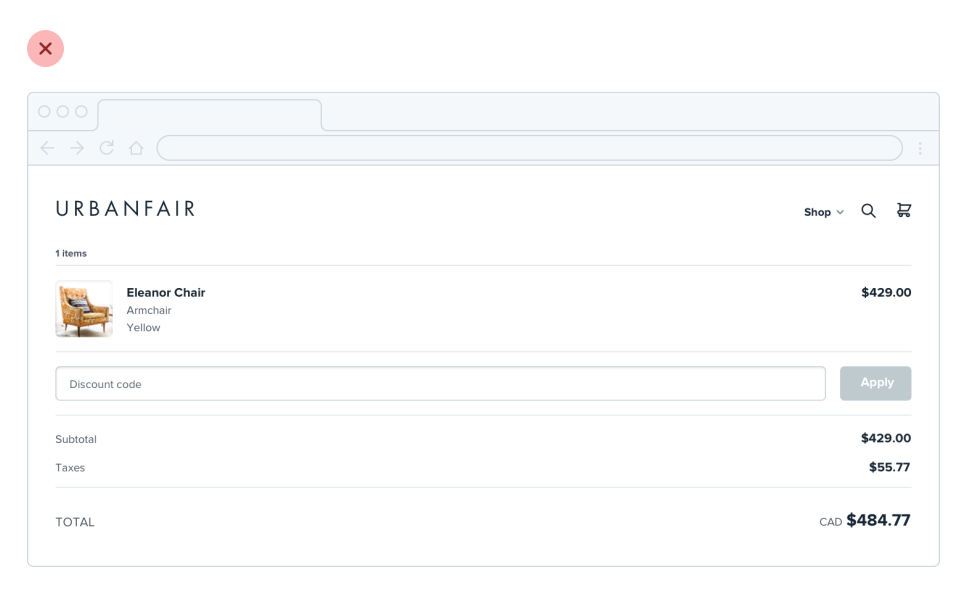
\includegraphics[keepaspectratio, width=12cm]{gambar/g-117.png}
	\caption{Komponen mengisi seluruh \textit{white space} dari sebuah halaman \citep{refactoringui}}
	\label{gambar:g-117.png}
\end{figure}

\begin{figure}[H]
	\centering
	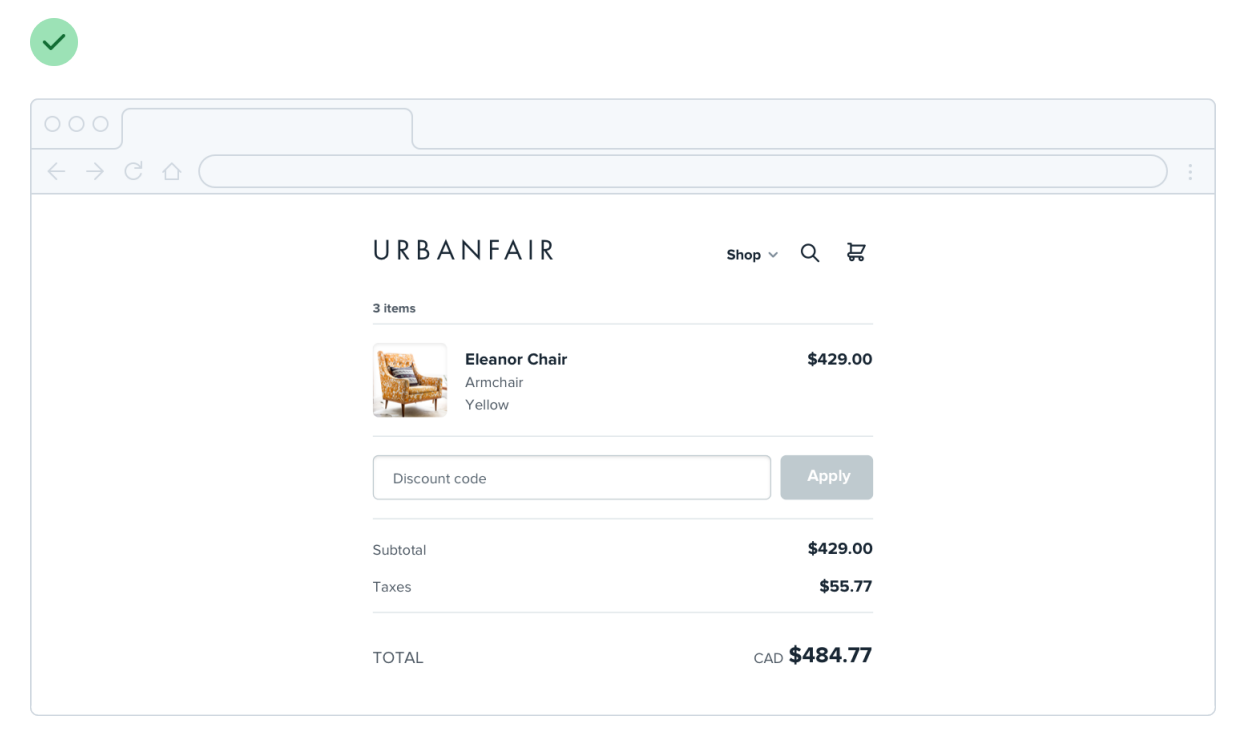
\includegraphics[keepaspectratio, width=14cm]{gambar/g-118.png}
	\caption{Komponen mengisi sebagian \textit{white space} dari sebuah halaman \citep{refactoringui}}
	\label{gambar:g-118.png}
\end{figure}

\subsubsection{Penentuan sistem desain \textit{spacing} dan \textit{sizing }}
%
%Dalam menentukan desain sistem untuk \textit{spacing} dan \textit{spacing} bukanlah hal yang mudah, dalam penentuannya tidaklah harus memilih-milih diantara dua ukuran atau lebih ukuran mana yang lebih baik atau lebih buruk, mencoba-coba beberapa ukuran untuk menemukan ukuran yang cocok adalah hal yang membuang waktu atau lebih parahnya lagi, membuat desain yang tidak konsisten. Pendekatan naif seperti memastikan ukuran \textit{spacing} dan \textit{sizing} dalam kelipatan 4 pixel tidaklah membantu permasalahan yang telah disebutkan. Dalam pembuatan sistem desain perlu diperhatikan hal seperti perbandingan relatif diantara dua nilai yang berdekatan. Contohnya adalah dalam skala kecil, penambahan beberapa \textit{pixel} dapat membuat perbedaan yang signifikan. Perubahan ukuran dari 12 \textit{pixel} ke 16 \textit{pixel} merupakan perubahan yang besar karena adanya 33 persen kenaikan.
%
%\begin{figure}[H]
%	\centering
%	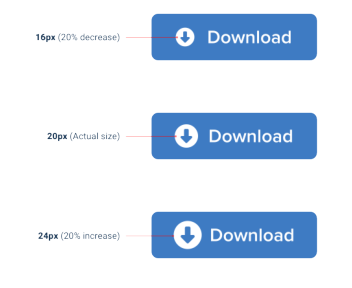
\includegraphics[keepaspectratio, width=12cm]{gambar/refactoring-ui-g4.png}
%	\caption{Perubahan pixel dalam skala kecil}
%	\label{gambar:refactoring-ui-g4.png}
%\end{figure}
%
%Akan tetapi dalam skala besar, perubahan beberapa \textit{pixel} adalah perubahan yang nyaris tidak terlihat, seperti perubahan ukuran dari 500 \textit{pixel} ke 520 \textit{pixel}, walaupun ada perbedaan 20 \textit{pixel} pada dua ukuran tersebut, perbedaan tersebut hanyalah 4 persen, 8 kali lipat kurang dari perubahan ukuran dari 12 \textit{pixel} ke 16 \textit{pixel}. Untuk mempermudah menentukan angka \textit{sizing} dan \textit{spacing}, pastikan saja ukuran diantara dua nilai tidak melebihi dari 25 persen. 
%
%\begin{figure}[H]
%	\centering
%	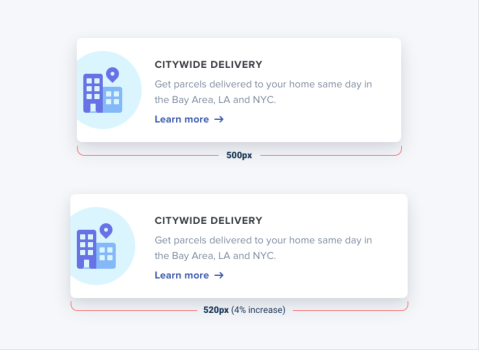
\includegraphics[keepaspectratio, width=12cm]{gambar/refactoring-ui-g3.png}
%	\caption{Perubahan pixel dalam skala besar}
%	\label{gambar:refactoring-ui-g3.png}
%\end{figure}

Dalam menentukan sebuah desain sistem ukuran \textit{sizing} dan \textit{spacing} tampilan, menghabiskan waktu dalam menentukan antara dua atau lebih nilai mana yang lebih baik untuk digunakan merupakan hal yang memakan waktu daripada menggunakan sistem yang telah ditentukan terlebih dahulu. Terdapat suatu pendekatan untuk menyelesaikan masalah tersebut dengan memulai dari menentukan nilai basis, dari nilai basis tersebut dapat dibuat rangkaian nilai skala dengan cara menggunakan nilai faktor dan mengalikannya dengan nilai basis yang telah ditentukan. Menggunakan nilai 16 \textit{pixel} sebagai basisnya disarankan dikarenakan 16 \textit{pixel} dapat dibagi secara baik dan merupakan setelan ukuran \textit{font browser} awal. Berikut ini merupakan contoh dari pendekatan yang telah disebutkan:

\begin{figure}[H]
	\centering
	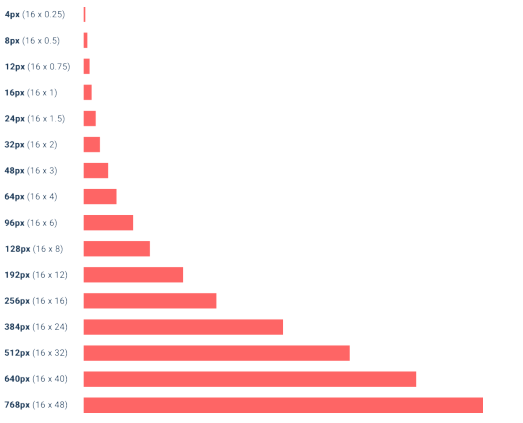
\includegraphics[keepaspectratio, width=8cm]{gambar/refactoring-ui-g5.png}
	\caption{Rangkaian nilai skala \citep{refactoringui}}
	\label{gambar:refactoring-ui-g5.png}
\end{figure}

\subsection{Text}
Kebanyakan tampilan yang ada menggunakan banyak sekali ukuran \textit{font}, bukan hal yang biasa untuk menemukan ukuran font dari ukuran 10 \textit{pixel} sampai 24 \textit{pixel} dalam satu tampilan. Hal ini merupakan hal yang tidak disarankan karena dua hal, desain yang tidak konsisten dan melambat pekerjaan.
\\
\begin{figure}[H]
	\centering
	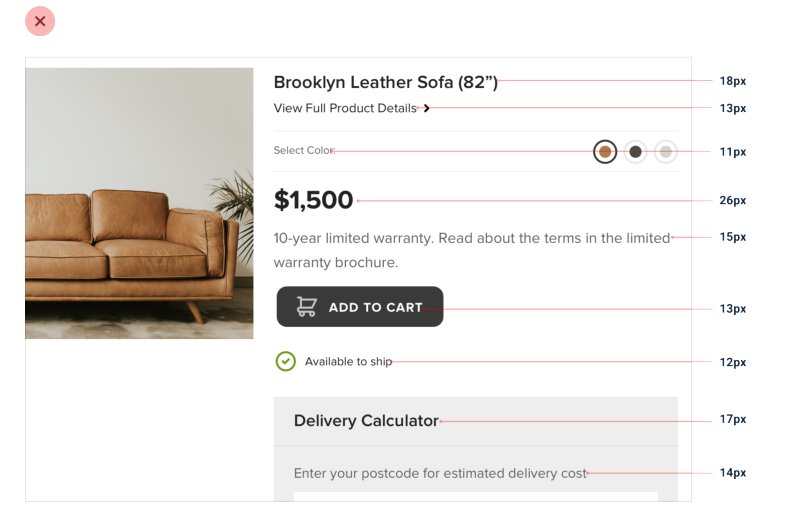
\includegraphics[keepaspectratio, width=8cm]{gambar/g100.png}
	\caption{Penggunaan ukuran font yang berlebihan dalam tampilan \citep{refactoringui}}
	\label{gambar:g100.png}
\end{figure}

%Dalam mendesain sistem desain untuk \textit{font}, sama seperti menentukan sistem desain {spacing dan sizing}, skala linear tidak dapat digunakan. 
Dalam membuat sistem desain font ada dua cara yaitu dengan menggunakan skala modular dan skala buatan sendiri.

Dalam skala modular, digunakan rasio seperti 4:5 ("\emph{a major third}"), 2:3 ("\emph{perfect fifth}") dan 1:1.618 ("\emph{golden ration}"). Dimulai dari menentukan nilai basis, mengaplikasikan rasio untuk mendapatkan angka selanjutnya dan mengaplikasikan nilai rasio tersebut lagi untuk mendapatkan nilai selanjutnya dan seterusnya. Pendekatan ini tampaknya menjanjikan, tapi dalam praktiknya, metode ini tidaklah sempurna karena beberapa alasan:

\begin{enumerate}
	\item{Dengan menggunakan skala modular dalam menentukan desain sistem \textit{font}, ukuran skala akan berakhir menggunakan angka pecahan, seperti  31.25 \textit{pixel}, 39.063 \textit{pixel}, 48.828 \textit{pixel} dan lain lainnya. \textit{Browser} menangani \textit{subpixel} sedikit berbeda sehingga nilai pecahan untuk ukuran text sebaiknya dihindari}.
	\item {Dengan menggunakan metode ini, ukuran skala yang dihasilkan adalah seperti 12 \textit{pixel}, 16 \textit{pixel}, 21 \textit{pixel} dan 28 \textit{pixel}. Hal ini membuat pemilihan ukuran font mejadi terbatas, pada praktiknya biasanya dibutuhkan nilai antara 21 \textit{pixel} dan 28 \textit{pixel} atau nilai antara 12 \textit{pixel} dan 16 \textit{pixel}}.
\end{enumerate}

\begin{figure}[H]
	\centering
	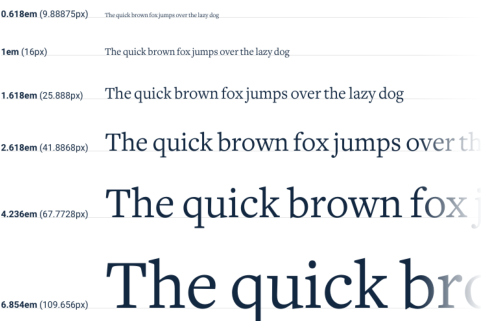
\includegraphics[keepaspectratio, width=12cm]{gambar/refactoring-ui-g6.png}
	\caption{Menentukan skala font menggunakan metode modular \citep{refactoringui}}
	\label{gambar:refactoring-ui-g6.png}
\end{figure}

Dalam skala buatan sendiri, penentuan nilai skala tidak dibatasi oleh formula matematika tetapi nilai skala ditentukan oleh pendesainnya sendiri. Dalam menggunakan metode ini tidak perlu lagi memerhatikan masalah seperti \textit{subpixel rounding} pada \textit{browser} dan juga dalam menggunakan metode ini, pendesain mempunyai kendali penuh dalam menentukan ukuran skala yang ada.

\begin{figure}[H]
	\centering
	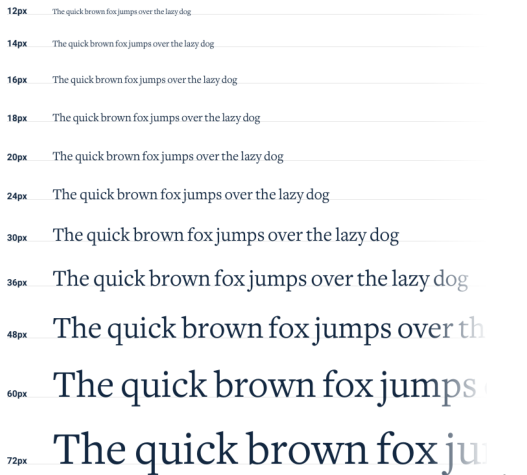
\includegraphics[keepaspectratio, width=12cm]{gambar/refactoring-ui-g7.png}
	\caption{Skala metode buatan sendiri \citep{refactoringui}}
	\label{gambar:refactoring-ui-g7.png}
\end{figure}

Pemilihan font yang akan digunakan dari ribuan \textit{font} yang tersedia secara tepat adalah hal yang sangat memakan waktu, kemampuan untuk melihat dan menentukan \textit{font} yang baik adalah kemampuan yang tidak dapat didapatkan secara singkat. Ada beberapa cara cepat untuk menentukan \textit{font} yang baik guna mengurangi waktu yang diperlukan untuk mempercepat proses pemilihan \textit{font} yaitu. 

\begin{enumerate}
	\item Untuk desain tampilan, pilihan yang aman adalah menggunakan \textit{typeface sans-serif} seperti Helvetica. Jika ragu untuk menggunakan \textit{font} yang dipilih, \textit{font} bawaan dari perangkat pengguna adalah pilihan tepat. Penggunaan \textit{font} dari bawaan perangkat pengguna membuat pengguna lebih familiar dengan tampilan yang dibuat karena pengguna sudah terbiasa dengan \textit{font} yang digunakan di perangkat meraka.
	\item Biasanya, \textit{font} didesain untuk tujuan yang spesifik. \textit{Font} yang memiliki \textit{letter-spacing} yang lebih rapat dan huruf \textit{lowercase} yang lebih pendek (\textit{shorter x-height}) biasanya digunakan untuk \textit{headline}, \textit{font} ini tidak cocok untuk digunakan sebagai \textit{font} utama dari tampilan . Sementara untuk \textit{font} yang digunakan untuk ukuran kecil seperti \textit{body} biasanya mempunyai \textit{letter-spacing} yang lebih lebar dan \textit{lowercase} letter yang lebih tinggi (\textit{taller x-height}).
	\begin{figure}[H]
		{\centering
			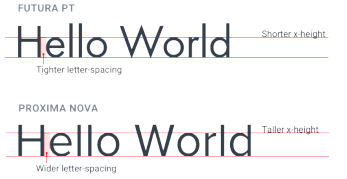
\includegraphics[keepaspectratio, width=12cm]{gambar/refactoring-ui-g9.png}
			\caption{Perbandingan \textit{font} untuk \textit{headline} dan \textit{body} \citep{refactoringui}}}
		\label{gambar:refactoring-ui-g9.png}
	\end{figure}
	\item Font yang populer kemungkinan besar adalah font yang bagus. Beberapa penyedia font di internet menyediakan fitur untuk mengurutkan font menurut urutan popularitas nya sehingga dapat mengurangi jumlah font yang harus dipilih.
	\begin{figure}[H]
		{\centering
			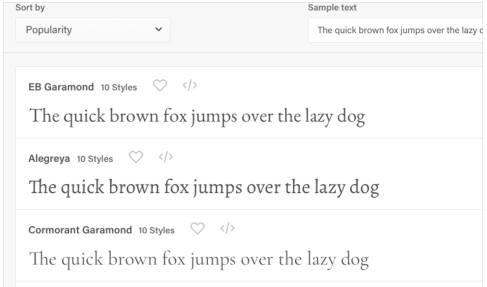
\includegraphics[keepaspectratio, width=12cm]{gambar/refactoring-ui-g10.png}
			\caption{Pengurutan berdasarkan popularitas \textit{font} \citep{refactoringui}}}
		\label{gambar:refactoring-ui-g10.png}
	\end{figure}
	\item Dimulai dengan mengunjungi beberapa situs favorit, biasanya dibalik situs tersebut, terdapat tim yang terdiri dari beberapa orang yang memiliki pengetahuan yang kuat tentang \textit{typography}. 
\end{enumerate}

Ketika mendesain paragraf, mudah sekali untuk membuat kesalahan dengan memuat seluruh teks ke dalam \textit{layout} yang ada dibandingkan dengan mencoba untuk membuat tampilan yang ramah untuk pembaca yang artinya teks akan terlihat sangat panjang dan sulit untuk dibaca.
\begin{figure}[H]
	{\centering
		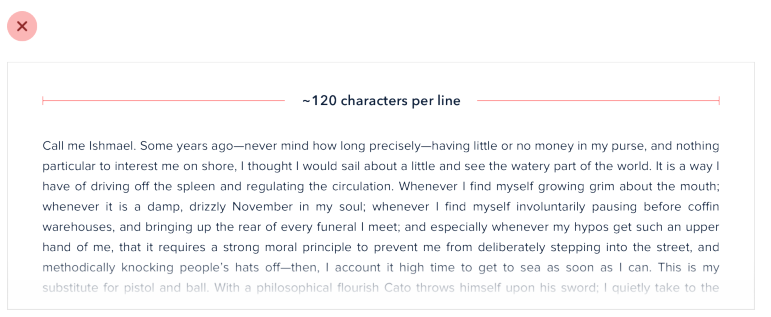
\includegraphics[keepaspectratio, width=16cm]{gambar/refactoring-ui-g11.png}
		\caption{Memuat banyak tulisan dalam sebuat \textit{layout} yang ada \citep{refactoringui}}}
	\label{gambar:refactoring-ui-g11.png}
\end{figure}

Untuk pengalaman membaca yang baik, paragraf haruslah dibuat untuk dapat menampung 45 sampai 75 karakter. Cara yang mudah dalam \textit{web} adalah menggunakan satuan unit \textit{em}, yang dimana satuan unit ini relatif dengan ukuran font \textit{web}. Ukuran yang tepat untuk ini adalah 20 \textit{em} sampai 35 \textit{em}.

\begin{figure}[H]
	{\centering
		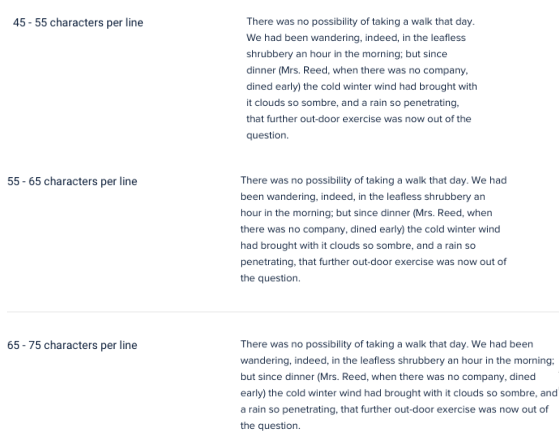
\includegraphics[keepaspectratio, width=14cm]{gambar/refactoring-ui-g12.png}
		\caption{Tampilan paragraf untuk ukuran 45-75 karakter \citep{refactoringui}}}
	\label{gambar:refactoring-ui-g12.png}
\end{figure}

Jika paragraf mengandung konten seperti gambar atau komponen yang besar, lebar text paragraf haruslah tetap dibatasi meskipun keseluruhan konten paragraf harus melebihi dari batas untuk menampung keseluruhan komponen.

\begin{figure}[H]
	{\centering
		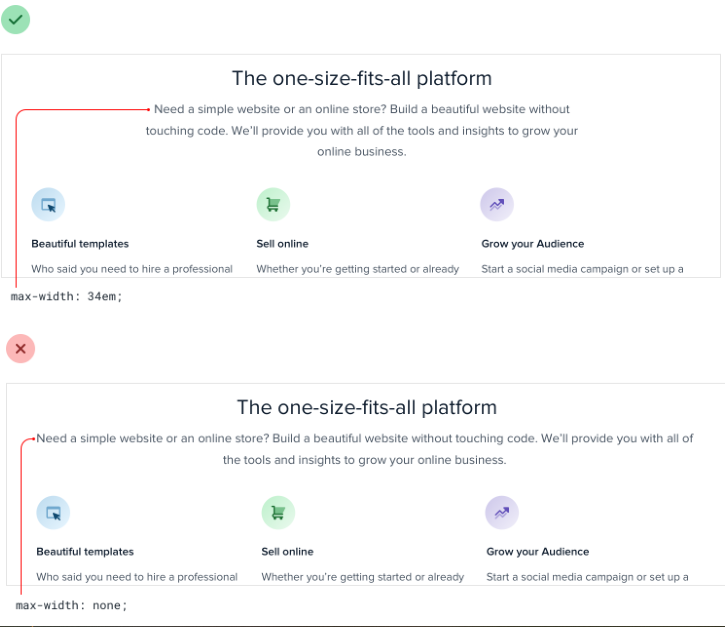
\includegraphics[keepaspectratio, width=12cm]{gambar/refactoring-ui-g13.png}
		\caption{Teks dengan komponen yang lebar dalam satu layout \citep{refactoringui}}}
	\label{gambar:refactoring-ui-g13.png}
\end{figure}

\subsubsection{\textit{Text Align}} 
Ada banyak situasi dimana diharuskan menggunakan beberapa ukuran \textit{font} dalam satu baris. Sebagai contoh dalam mendesain kartu dimana judul kartu tersebut memerlukan ukuran font yang lebih besar dibandingkan dengan elemen di sampingnya. Saat mencampur ukuran font seperti ini, biasanya secara insting, desainer akan cenderung melakukan \textit{center}-ing terhadap komponen tersebut untuk menciptakan keseimbangan.

 \begin{figure}[H]
	{\centering
		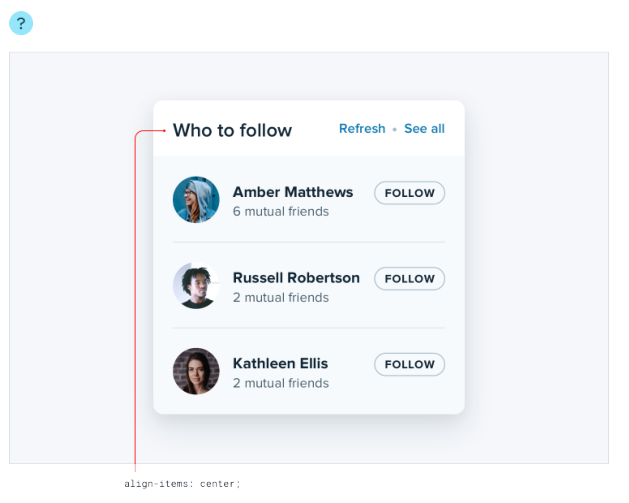
\includegraphics[keepaspectratio, width=10cm]{gambar/refactoring-ui-g14.png}
		\caption{Komponen kartu \citep{refactoringui}}}
	\label{gambar:refactoring-ui-g14.png}
\end{figure}

Ketika ada banyak ruang diantara dua komponen, hal ini terlihat baik baik saja. Namun jika kedua komponen teks tersebut didekatkan maka akan menjadi jelas bahwa tampilan akan terlihat buruk.
\begin{figure}[H]
	{\centering
		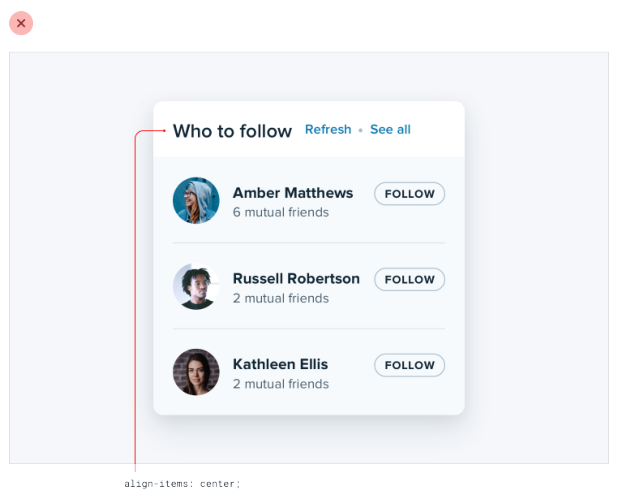
\includegraphics[keepaspectratio, width=10cm]{gambar/refactoring-ui-g17.png}
		\caption{Komponen kartu dengan komponen aksi dan judul didekatkan \citep{refactoringui}}}
	\label{gambar:refactoring-ui-g17.png}
\end{figure}

Pendekatan terbaik adalah menyelaraskan kedua komponen tersebut dengan \textit{baseline} atau sebuah garis imajinari tempat teks berdiri yang digunakan oleh teks untuk berdiri.
\begin{figure}[H]
	{\centering
		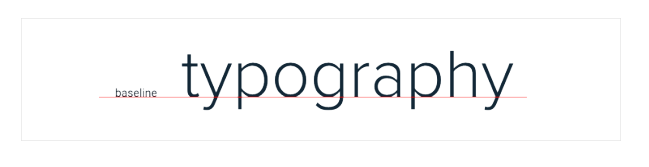
\includegraphics[keepaspectratio, width=12cm]{gambar/refactoring-ui-g18.png}
		\caption{\textit{Baseline} \citep{refactoringui}}}
	\label{gambar:refactoring-ui-g18.png}
\end{figure}
\begin{figure}[H]
	{\centering
		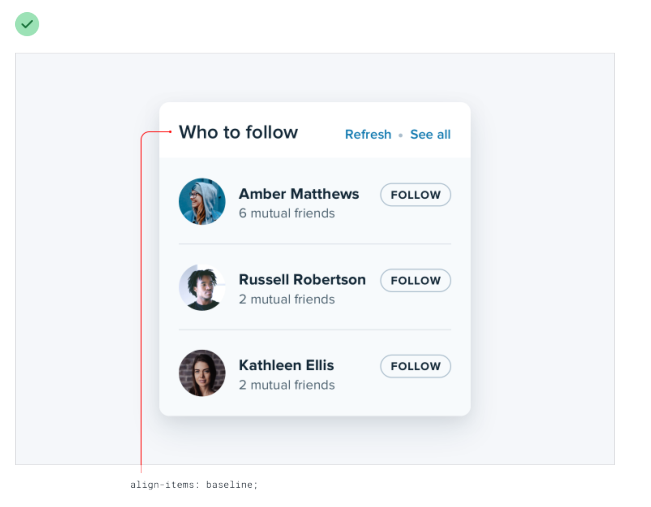
\includegraphics[keepaspectratio, width=12cm]{gambar/refactoring-ui-g19.png}
		\caption{Komponen aksi dan judul diselaraskan menurut \textit{baseline} \citep{refactoringui}}}
	\label{gambar:refactoring-ui-g19.png}
\end{figure}

\subsubsection{Letter spacing}
Pada umumnya ada baiknya untuk mempercayakan \textit{letter spacing} kepada pendesain \textit{font} tersebut. Namun ada beberapa kasus yang dimana mengubah \textit{letter spacing} dapat memperindah tampilan yang ada.
 \begin{figure}[H]
	{\centering
		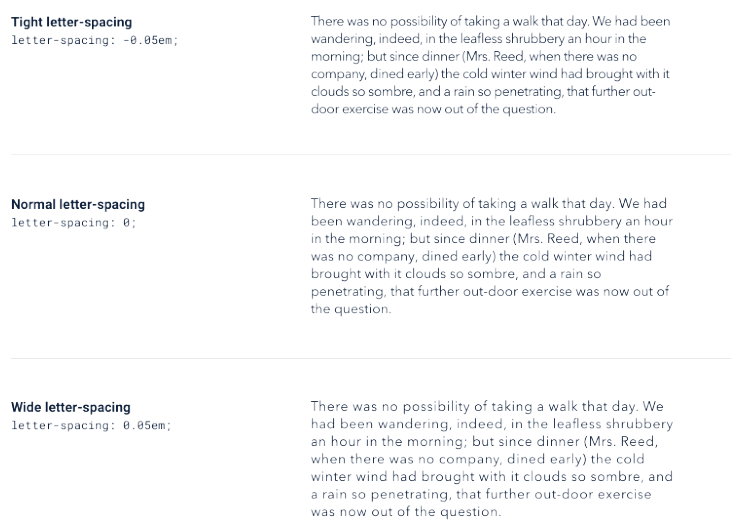
\includegraphics[keepaspectratio, width=12cm]{gambar/refactoring-ui-g21.png}
		\caption{\textit{Letter spacing} \citep{refactoringui}}}
	\label{gambar:refactoring-ui-g21.png}
\end{figure}
Ketika seseorang mendesain sebuah font, mereka mendesain \textit{font} tersebut dengan tujuan tertentu. \textit{Font family} seperti Open Sans didesain untuk keterbacaan dalam ukuran kecil yang dimana \textit{letter spacing} dari font family tersebut terlihat lebih besar dibandingkan dengan \textit{font family} seperti Oswald, yang dimana \textit{font family} Oswald digunakan untuk kebutuhan seperti penulisan judul utama.

\begin{figure}[H]
	{\centering
		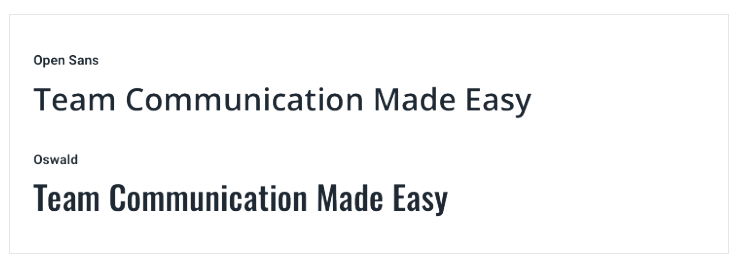
\includegraphics[keepaspectratio, width=12cm]{gambar/refactoring-ui-g22.png}
		\caption{\textit{Font family} Open Sans dan Oswald \citep{refactoringui}} }
	\label{gambar:refactoring-ui-g22.png}
\end{figure}

\textit{Font} yang dikhususkan untuk keterbacaan dalam ukuran kecil seperti Open Sans juga dapat digunakan untuk penulisan judul utama. Dengan mengurangi \textit{letter spacing} untuk meniru fungsi dari \textit{font family} seperti Oswald. Namun, hindari penggunaan sebaliknya, penggunaan \textit{font family} judul utama untuk keterbacaan dalam ukuran kecil memiliki kemungkinan kecil untuk bekerja.  

\begin{figure}[H]
	{\centering
		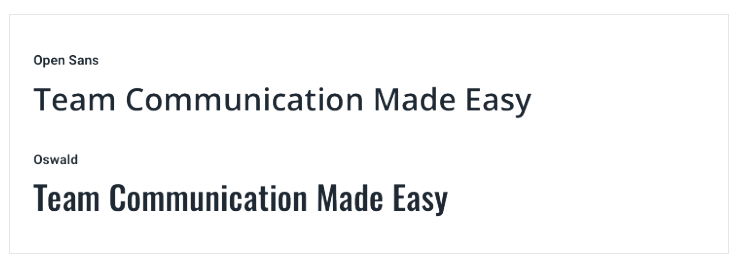
\includegraphics[keepaspectratio, width=12cm]{gambar/refactoring-ui-g22.png}
		\caption{\textit{Font family} Open Sans digunakan untuk \textit{headline} \citep{refactoringui}}}
	\label{gambar:refactoring-ui-g23.png}
\end{figure}

\subsection{Warna}
\subsubsection{\textit{Color Palette}}
\textit{Color palette} dapat dibagi menjadi tiga kelompok yaitu
\begin{enumerate}
	\item \emph{Abu abu} \hfill\\
	Warna yang biasanya terdapat pada beberapa komponen tampilan seperti \textit{form}, panel, warna latar belakang dan teks.
	\item \emph{Warna utama (\textit{primary color})} \hfill\\
	Warna yang digunakan dalam komponen seperti \textit{button}, navigasi dan lain lain. Warna ini mendefinisikan bagaimana suatu website terlihat, seperti contohnya ketika memikirkan sebuah merek seperti Facebook maka akan terpikirkan warna biru yang merupakan ciri khas dari Facebook sendiri.
	\item \emph{Warna aksen (\textit{accent color})} \hfill\\
	Warna aksen digunakan untuk menyampaikan maksud tertentu terhadap pengguna. Sebagai contoh, warna merah atau jingga digunakan untuk memikat pengguna terhadap fitur baru yang baru saja dirilis atau seperti warna merah yang digunakan untuk meminta konfirmasi pengguna untuk aksi yang destruktif.
	\begin{figure}[H]
		{\centering
			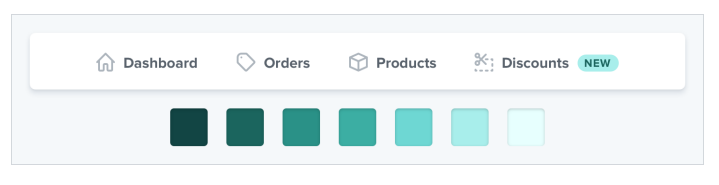
\includegraphics[keepaspectratio, width=12cm]{gambar/refactoring-ui-33.png}
			\caption{Penggunaan warna aksen untuk informasi \citep{refactoringui}}}
		\label{gambar:refactoring-ui-33.png}
	\end{figure}
	\begin{figure}[H]
		{\centering
			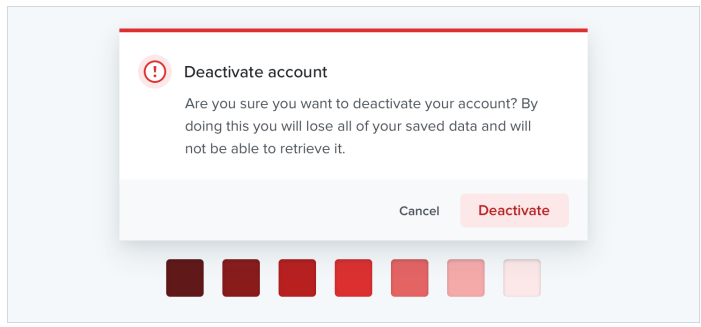
\includegraphics[keepaspectratio, width=12cm]{gambar/refactoring-ui-34.png}
			\caption{Penggunaan warna aksen untuk aksi destruktif \citep{refactoringui}}}
		\label{gambar:refactoring-ui-34.png}
	\end{figure}
\end{enumerate}

\subsubsection{Menentukan warna \textit{shade}} \textit{Shade} dapat ditentukan dari warna basis yang ada. Warna basis merupakan warna yang berada di tengah tengah antara shade yang paling gelap dan shade yang paling terang. Dalam penentuan basis warna sendiri, tidak ada formula khusus, melainkan terdapat beberapa cara yang dapat dipakai dalam menentukan basis warna. Caranya adalah mengambil basis warna shade yang cocok digunakan untuk warna \textit{background} dari elemen \textit{button}.
\begin{figure}[H]
	{\centering
		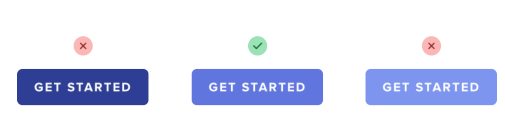
\includegraphics[keepaspectratio, width=12cm]{gambar/refactoring-ui-g40.png}
		\caption{Menentukan warna basis yang tepat menggunakan komponen \textit{button} \citep{refactoringui}}}
	\label{gambar:refactoring-ui-g40.png}
\end{figure}

Selanjutnya adalah menentukan sisi paling gelap dan sisi paling terang, dalam menentukan sisi yang paling gelap dan sisi yang paling terang dari warna shade tidak ada formula khusus yang dapat digunakan. Biasanya, sisi yang paling gelap digunakan untuk sebuah teks sedangkan sisi yang paling terang digunakan untuk sebuah \textit{background}. Dalam penentuannya dapat dimulai dengan menentukan basis warna lalu mengatur atribut \textit{saturation} dan \textit{lightness} hingga dirasa cocok.

\begin{figure}[H]
	{\centering
		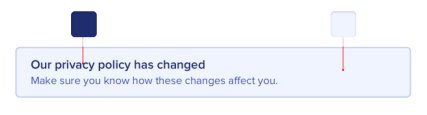
\includegraphics[keepaspectratio, width=12cm]{gambar/refactoring-ui-41.png}
		\caption{\textit{Shade} tergelap dan terterang \citep{refactoringui}}}
	\label{gambar:refactoring-ui-41.png}
\end{figure}

Saat selesai menentukan basis warna dan \textit{shade} warna paling gelap dan paling terang, langkah selanjutnya adalah mengisi ruang kosong yang ada. Pada umumnya, dibutuhkan sekurang kurangnya 5 warna \textit{shade} dalam suatu projek dan kurang lebih 10 warna \textit{shade} jika tidak ingin merasa dibatasi dengan pilihan warna. Angka 9 adalah angka yang tepat dikarenakan mudah untuk dibagi dan membuat mengisi ruang kosong yang ada lebih mudah. 900 adalah warna \textit{shade} paling gelap, 100 paling terang dan 500 adalah basis warna.

\begin{figure}[H]
	{\centering
		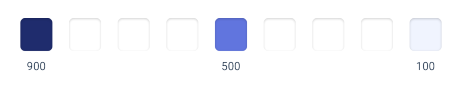
\includegraphics[keepaspectratio, width=12cm]{gambar/refactoring-ui-42.png}
		\caption{Nilai \textit{shade} untuk basis warna \citep{refactoringui}}}
	\label{gambar:refactoring-ui-42.png}
\end{figure}

Pengisian dimulai dari angka 700 dan 300 karena angka inilah yang berada di tengah tengah ruang kosong terus lanjutkan hingga semua ruang kosong terisi.

\begin{figure}[H]
	{\centering
		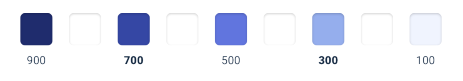
\includegraphics[keepaspectratio, width=12cm]{gambar/refactoring-ui-43.png}
		\caption{Pengisian nilai \textit{shade} untuk nilai 300 dan 700 \citep{refactoringui}}}
	\label{gambar:refactoring-ui-43.png}
\end{figure}

\begin{figure}[H]
	{\centering
		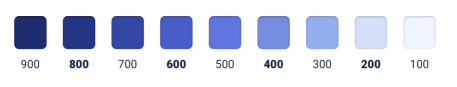
\includegraphics[keepaspectratio, width=12cm]{gambar/refactoring-ui-44.png}
		\caption{Pengisian nilai \textit{shade} untuk nilai 200, 400, 600 dan 700 \citep{refactoringui}}}
	\label{gambar:refactoring-ui-44.png}
\end{figure}

\subsubsection{\textit{HSL}} Hex dan RGB adalah dua format warna yang umum digunakan pada tampilan. Warna warna \textit{hex} dapat memiliki tampilan warna yang terlihat sama namun jika dilihat dari representasi kodenya, mereka terlihat tidak sama. HSL menyelesaikan masalah ini dengan mempresentasikan warna dengan atribut yang orang orang dapat merasakannya secara intuitif. Atribut yang dimaksud adalah \textit{hue}, \textit{saturation} dan \textit{lightness}.


\begin{figure}[H]
	{\centering
		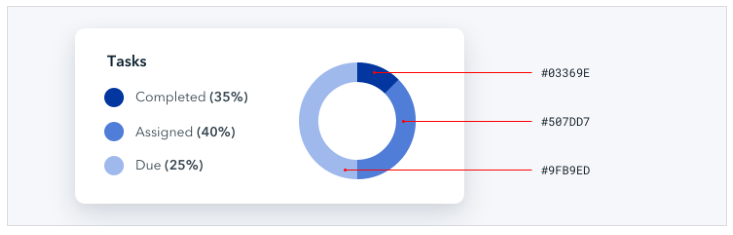
\includegraphics[keepaspectratio, width=12cm]{gambar/refactoring-ui-g24.png}
		\caption{Penggunaan \textit{hex} \citep{refactoringui}}}
	\label{gambar:refactoring-ui-g24.png}
\end{figure}

\begin{figure}[H]
	{\centering
		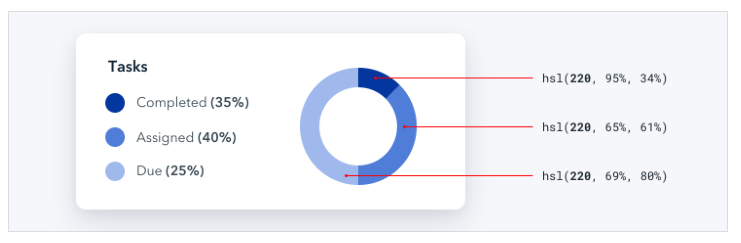
\includegraphics[keepaspectratio, width=12cm]{gambar/hsl-1.png}
		\caption{Penggunaan \textit{hsl} \citep{refactoringui}}}
	\label{gambar:hsl-1.png}
\end{figure}

\textit{Hue} merupakan atribut yang merupakan posisi warna di \textit{color wheel}. \textit{Hue} diukur dalam satuan derajat yang dimana 0 derajat melambangkan merah, 120 derajat melambangkan hijau dan 240 derajat melambangkan biru.
\begin{figure}[H]
	{\centering
		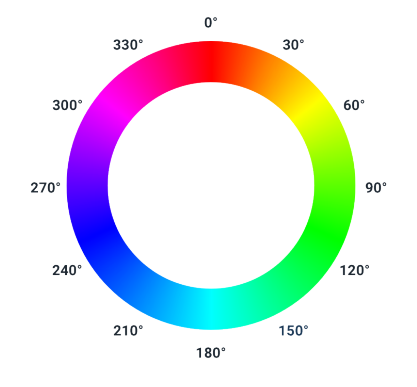
\includegraphics[keepaspectratio, width=12cm]{gambar/refactoring-ui-30png.png}
		\caption{\textit{Hue} \citep{refactoringui}}}
	\label{gambar:refactoring-ui-30png.png}
\end{figure}

\textit{Saturation} adalah nilai yang mengukur seberapa mencolok atau jelas suatu warna, 0\% \textit{saturation} menandakan warna abu abu (tidak ada warna),  sedangkan \textit{saturation} 100\% menandakan warna yang mencolok dan jelas. Tanpa \textit{saturation} nilai \textit{hue} tidaklah bermakna seberapapun nilainya karena warna akan tetap menjadi abu abu (tidak ada warna).
\begin{figure}[H]
	{\centering
		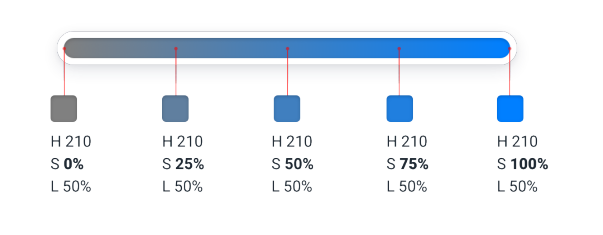
\includegraphics[keepaspectratio, width=12cm]{gambar/refactoring-ui-31.png}
		\caption{\textit{Saturation} \citep{refactoringui}}}
	\label{gambar:refactoring-ui-31.png}
\end{figure}

Atribut \textit{lightness} merupakan nilai yang mengukur seberapa dekat atau jauhnya sebuah warna dengan warna hitam maupun putih. 0\% \textit{lightness} adalah warna hitam, 100\% \textit{lightness} merupakan warna putih dan 50\% \textit{lightness} merupakan warna asli dalam nilai \textit{hue} tersebut.

\begin{figure}[H]
	{\centering
		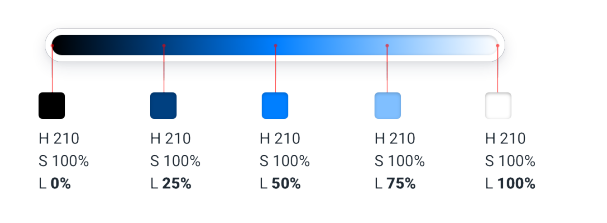
\includegraphics[keepaspectratio, width=12cm]{gambar/refactoring-ui-32.png}
		\caption{\textit{Lightness} \citep{refactoringui}}}
	\label{gambar:refactoring-ui-32.png}
\end{figure}

\subsubsection{\textit{Accessibility}}
Untuk mendesain tampilan yang \textit{accessible}, \textit{Web Content Accessibility Guidelines (WCAG)} merekomendasikan teks normal yang memiliki ukuran dibawah 18 \textit{pixel} memiliki kontras dengan perbandingan 4.5:1 dan teks yang lebih besar dari tersebut memiliki kontras tampilan setidaknya 3:1 untuk mendapat nilai kontras minimum (AA) dan kontras 7:1 untuk teks normal dibawah 18 dan 4.5:1 untuk teks yang lebih besar untuk mendapatkan nilai kontras yang tinggi (AAA).
\begin{figure}[H]
	{\centering
		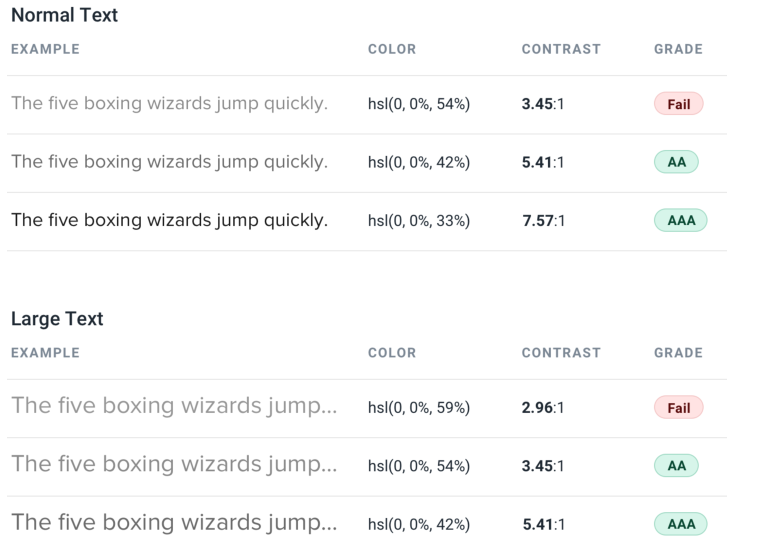
\includegraphics[keepaspectratio, width=12cm]{gambar/g-101.png}
		\caption{Kontras untuk teks ukuran normal dan besar \citep{refactoringui}}}
	\label{gambar:g-101.png}
\end{figure}

Untuk keperluan teks hitam diatas latar belakang yang cerah, memenuhi persyaratan perbandingan kontras yang direkomendasikan merupakan hal yang mudah. Namun, untuk memenuhi persyaratan yang direkomendasikan akan terasa sulit jika menggunakan warna. Ketika menggunakan teks putih diatas tampilan bewwarna diperlukan warna yang lebih gelap untuk memenuhi persyaratan kontras 4.5:1. 

\begin{figure}[H]
	{\centering
		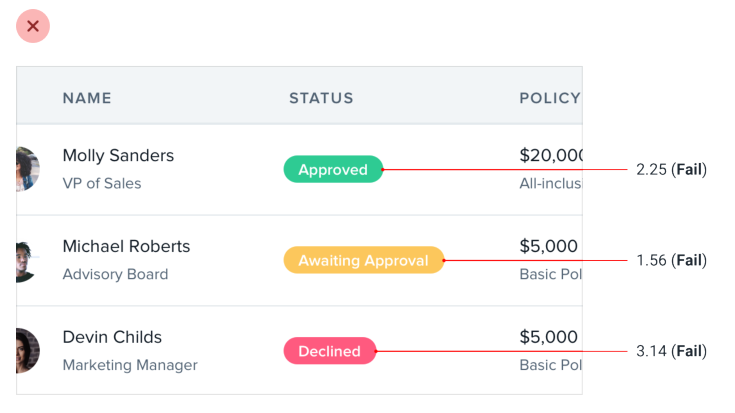
\includegraphics[keepaspectratio, width=12cm]{gambar/g-102.png}
		\caption{Teks putih diatas tampilan berwarna \citep{refactoringui}}}
	\label{gambar:g-102.png}
\end{figure}

Penambahan kegelapan warna dapat menimbulkan masalah hierarki kepada elemen yang seharusnya tidak menjadi fokus utama dari halaman. Latar belakang berwarna yang gelap akan mencuri perhatian pengguna.

\begin{figure}[H]
	{\centering
		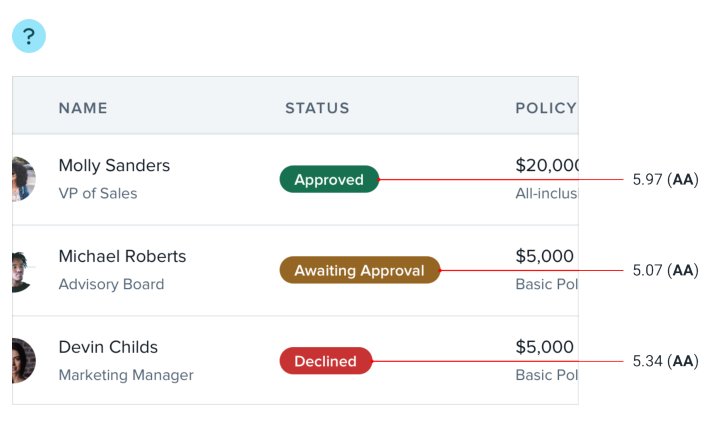
\includegraphics[keepaspectratio, width=12cm]{gambar/g-103.png}
		\caption{Tampilan warna yang gelap dapat mencuri perhatian pengguna \citep{refactoringui}}}
	\label{gambar:g-103.png}
\end{figure}

Permasalahan ini dapat diatasi dengan membalikan kontras. Daripada menggunakan teks dengan warna terang pada latar belakan berwarna gelap, menggunakan teks dengan warna gelap diatas latar belakang berwarna cerah merupakan pilihan yang tepat.

\begin{figure}[H]
	{\centering
		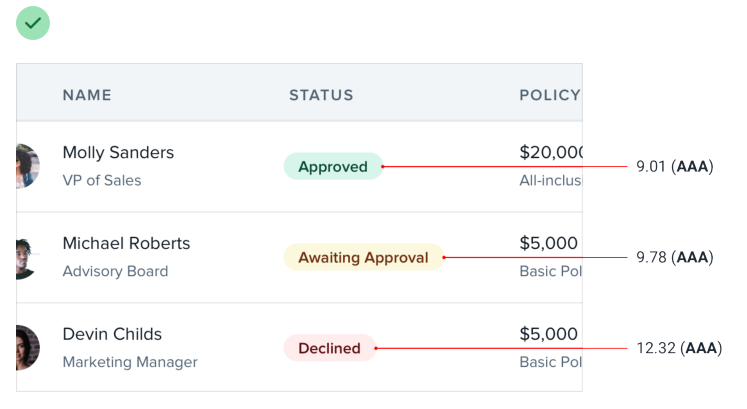
\includegraphics[keepaspectratio, width=8cm]{gambar/g-104.png}
		\caption{Pembalikan kontras antara teks dengan latar belakang \citep{refactoringui}}}
	\label{gambar:g-104.png}
\end{figure}

Untuk menyampaikan informasi kepada pengguna, warna saja tidaklah cukup dalam menyampaikan pengguna atau tidak pengguna dengan penyakit buta warna akan merasa kesulitan dalam menginterpretasikan tampilan yang ada. Sebagai contoh dalam gambar statistik di bawah ini, pengguna dengan buta warna hijau akan memiliki kesulitan dalam menentukan apakah statistik tersebut membaik atau memburuk.

\begin{figure}[H]
	{\centering
		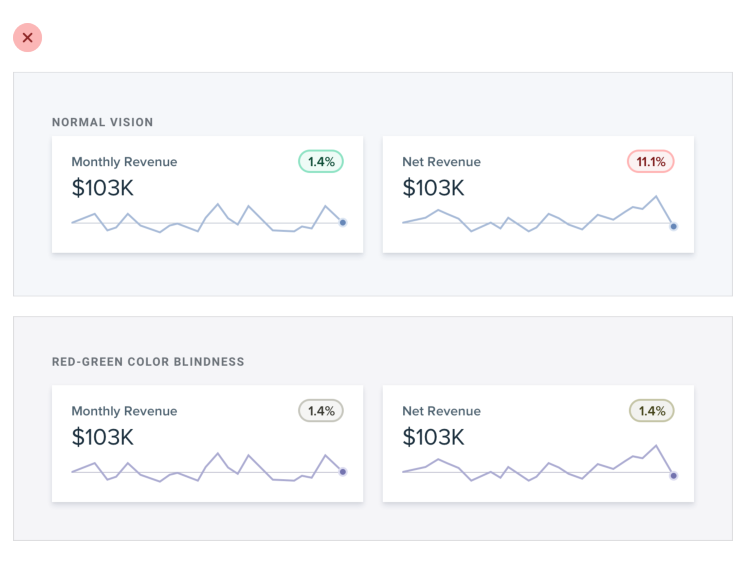
\includegraphics[keepaspectratio, width=8cm]{gambar/g-105.png}
		\caption{Warna saja tidak cukup dalam menyampaikan informasi \citep{refactoringui}}}
	\label{gambar:g-105.png}
\end{figure}

Untuk mengatasi masalah ini adalah dengan menambahkan cara lain untuk menyampaikan maksud kepada user, seperti menambahkan ikon yang mengindisakan perubahan positif atau negatif.

\begin{figure}[H]
	{\centering
		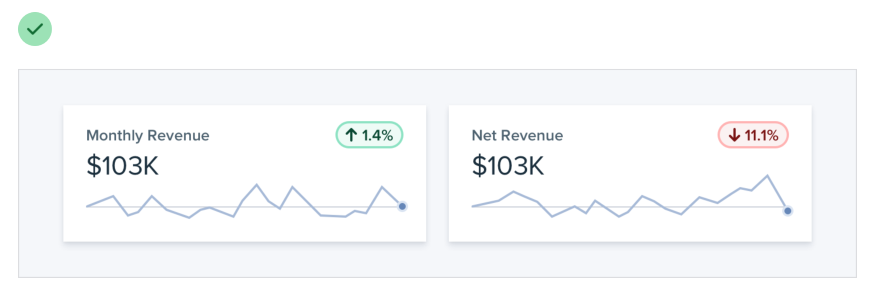
\includegraphics[keepaspectratio, width=12cm]{gambar/g-106.png}
		\caption{Penambahan ikon disamping warna untuk menyampaikan informasi \citep{refactoringui}}}
	\label{gambar:g-106.png}
\end{figure}

Untuk tampilan grafik yang terkadang memiliki banyak warna yang berbeda untuk setiap \textit{trend line}, akan lebih baik menggunakan perbedaan kontras daripada mengandalkan warna yang berbeda untuk setiap \textit{trend line}. Pengguna buta warna akan lebih mudah untuk mengenali perbedaan terang dan gelap dibandingkan dengan membedakan dua warna yang berbeda.
\begin{figure}[H]
	{\centering
		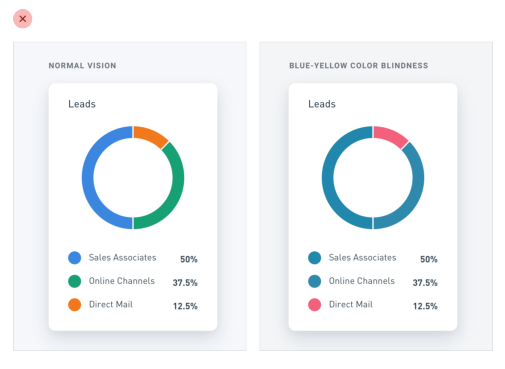
\includegraphics[keepaspectratio, width=10cm]{gambar/g-107.png}
		\caption{Menggunakan warna berbeda untuk setiap \textit{trend line} \citep{refactoringui}}}
	\label{gambar:g-107.png}
\end{figure}
\begin{figure}[H]
	{\centering
		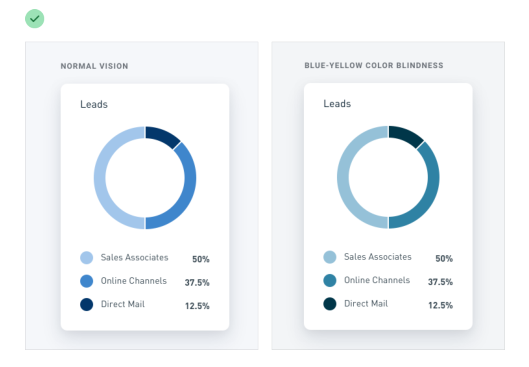
\includegraphics[keepaspectratio, width=10cm]{gambar/g-108.png}
		\caption{Menggunakan kontras yang berbeda untuk setiap \textit{trend line} \citep{refactoringui}}}
	\label{gambar:g-168.png}
\end{figure}


\section{Javascript}
\textit{Javascript} merupakan bahasa pemrograman tingkat tinggi dan bahasa pemrograman \textit{interpreted} yang biasanya digunakan untuk menambahkan interaktivitas dan sifat dinamis dalam sebuah \textit{websites}. Javascript biasa dikenal sebagai "Bahasa \textit{Web}" dikarenakan javascript didukung oleh mayoritas \textit{web browsers} dan dapat membuat elemen yang interaktif, memanipulasi konten sebuah \textit{website} dan merespon aksi pengguna.

Javascript di kembangkan oleh Brendan Eich pada tahun 1995 ketika Brendan Eich sedang bekerja pada perusahaan Netscape Communications Corporation. Pengembangan javascript dilakukan karena adanya kebutuhan bahasa \textit{scripting} yang dapat menambahkan interaksi dan fungsi dinamis dalam \textit{website}. Pada saat itu, kebanyakan \textit{website} merupakan statis dan kekurangan kemampuan dalam merespon interaksi pengguna.

Sebelummnya bernama "Mocha", bahasa ini kemudian berganti nama menjadi "Livescript" dan pada akhirnya "Javascript" untuk kebutuhan marketing, memanfaatkan popularitas bahasa pemrograman Java pada saat itu. Meskipun Javascript dan Java memiliki nama yang hampir mirip, keduanya merupakan bahsa yang berbeda dengan prinsip desain dan tujuan yang berbeda.

Seiring berkembangnya popularitas javascript, \textit{web browser} lainnya seperti Microsoft dengan Internet Explorer dan Mozilla dengan Firefox, mengimplementasikan dukungan untuk bahasa pemgrograman javascript. Adopsi javascript ke dalam \textit{web browser} terkenal tersebut membuat pendukung yang kuat bagi javascript untuk menjadi stndar \textit{de facto} untuk \textit{client-side scripting} pada \textit{website}.

Selama bertahun tahun, Javascript telah mengalami perubahan yang signifikan dengan adanya fitur-fitur baru, improvisasi dan penambahan pada bahasa Javascript. AJAX atau \textit{Asynchronous Javascript and XML} pada awal tahun 2000 mengembangkan kemampuan Javascript lebih jauh lagi dengan kemampuannya melakukan komunikasi \textit{asynchronous} dengan \textit{server} melakukan perubahan data yang dinamis pada halaman \textit{website} tanpa melakukan muat ulang halaman \textit{website}.

Dalam akhir akhir ini, Javascript telah berkembang melebihi dari kebutuhan aslinya. Dengan pengenalan NodeJS, program yang dapat menjalankan Javascript di luar browser. Dengan ini, Javascript dapat digunakan dalam berbagai bidang seperti \textit{server-side scripting}, \textit{command-line tools} dan membuat aplikasi. Javascript juga telah tumbuh lebih signifikan lagi dengan perkenalan berbagai \textit{framework}, \textit{library} dan \textit{tools} yang mensimplifikasikan proses pengembangan. \textit{Framework} popular sperti Angular, React dan VueJS telah diadopsi oleh banyak orang, memberikan pengembang alat untuk membuat aplikasi \textit{web} yang kompleks.

\section{Three JS}
Three.js merupakan sebuah library dari Javascript untuk
membuat dan menampilkan grafik 3D pada web browser. Dengan menggunakan Three JS, pembuatan tampilan 3 dimensi lebih mudah untuk dilakukan dikarenakan Three JS sudah menyediakan beberapa fitur seperti \textit{scenes}, \textit{camera}, \textit{lights}, \textit{shadows}, \textit{materials}, \textit{textures}, \textit{3d math} dan lain lain.
\subsection{\emph{Camera}}
\textit{Camera} mendefinisikan bagaimana apa yang akan kita lihat jika kita me-\textit{render} \textit{scene}. Jenis \textit{camera} yang paling banyak digunakan dalam three js adalah \textit{perspective camera} yang memberikan efek 3d dimana objek dekat terlihat lebih besar sedangkan objek yang letaknya jauh terlihat lebih kecil.
\textit{Perspective camera} mendefinisikan fructumnya melalui empat properties yaitu \textit{near} yang mendefinisikan dimana letak frustum depan, \textit{end} mendifinisikan dimana itu berakhir, \textit{fov} atau \textit{field of view} merupakan bagian dari scene yang dapat terlihat dari \textit{camera} dan \textit{aspect} merupakan perbandingan antara garis vertikal dan horizontal dari \textit{scene} yang akan ditampilkan.

\begin{figure}[H]
	\centering
	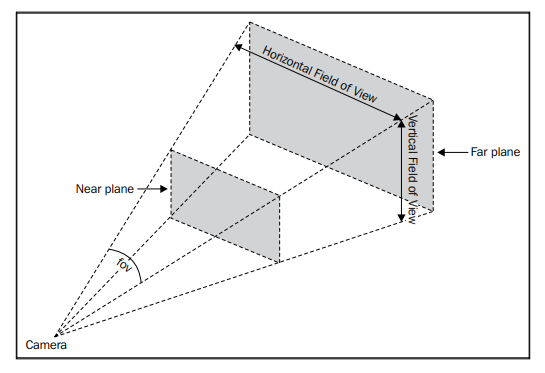
\includegraphics[keepaspectratio, width=12cm]{gambar/fructum}
	\caption{Frustum Camera ThreeJS}
	\label{gambar:fructum.png}
\end{figure}

\subsection{\emph{Mesh}}
Mesh merupakan objek triangular polygon yang dibuat dengan gabungan antara objek Geometry dan  Material. Mesg juga merupakan basis objek dari berbagai objek mesh lainnya seperti Skinned Mesh, MorhAnimMesh dan lain lain.
\begin{figure}[H]
	\centering
	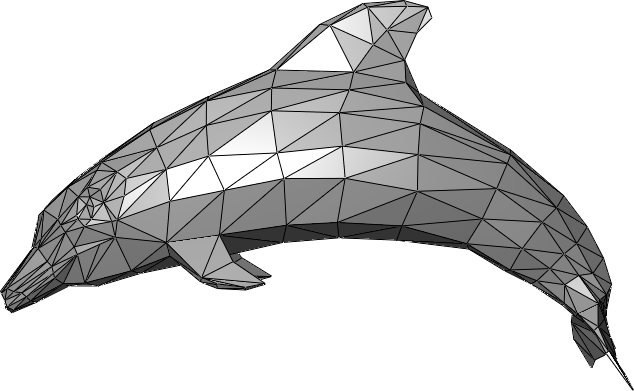
\includegraphics[keepaspectratio, width=8cm]{gambar/mesh.png}
	\caption{Mesh ThreeJS}
	\label{gambar:mesh.png}
\end{figure}

\subsection{\emph{Scene Graph}}
\textit{Scene graph} merupakan struktur seperti pohon yang terdiri dari beberapa objek seperti \textit{scene}, \textit{camera}, \textit{mesh} dan lain lain. Objek objek tersebut berstruktur secara hierarki dengan hubungan seperti \textit{parent} dan \textit{child} dan merepresentasikan dimana objek akan muncul dan bagaimana mereka berorientasi. \textit{Children} diposisikan dan diorientasikan sesuai dengan \textit{parent} mereka. 

\begin{figure}[H]
	\centering
	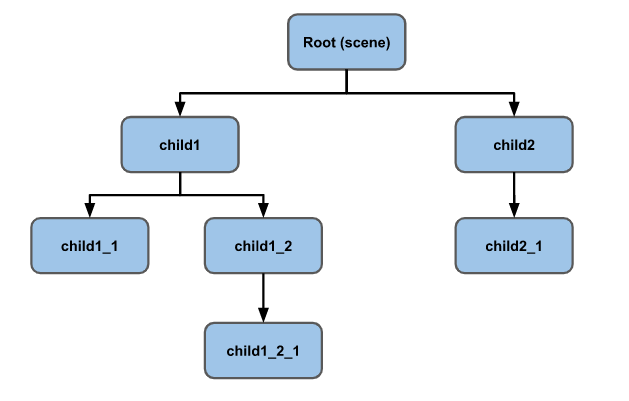
\includegraphics[keepaspectratio, width=12cm]{gambar/tree-graph-three}
	\caption{Scene Graph ThreeJS}
	\label{gambar:tree-graph-three.png}
\end{figure}

\subsection{\emph{Primitives}}
\textit{primitives} merupakan bentuk 3-dimensi yang dihasilkan saat program berjalan dengan beberapa parameter yang telah ditentukan. Three JS memiliki beberapa \textit{primitives} bawaan seperti \textit{BoxGeometry}, \textit{CircleGeometry}, \textit{CylinderGeometry}, \textit{ConeGeometry} dan lain lain dengan parameter yang dapat ditentukan untuk setiap masing masing bentuk sesuai dengan keinginan. 

\begin{figure}[H]
	\centering
	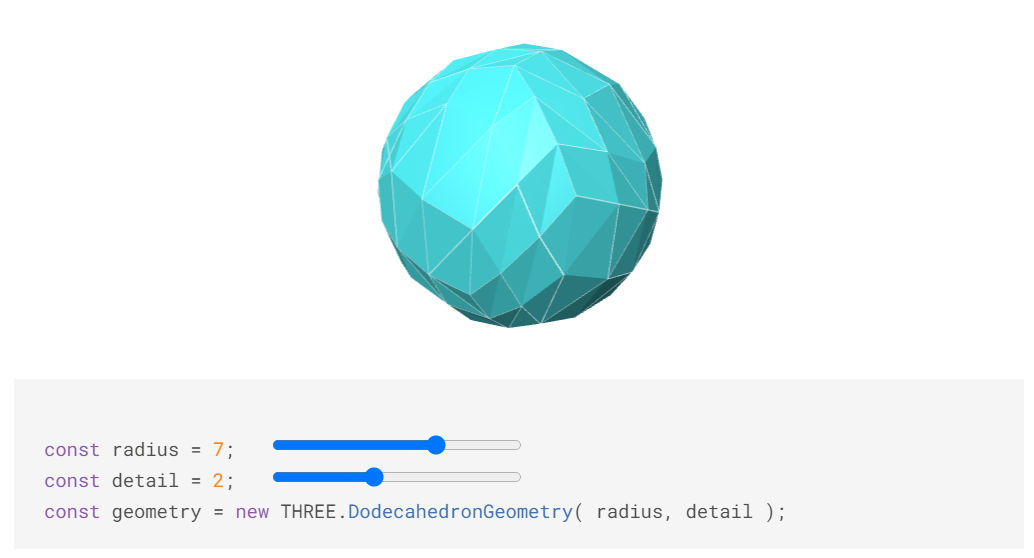
\includegraphics[keepaspectratio, width=12cm]{gambar/three-js-geometry-example.png}
	\caption{Primitives ThreeJS}
	\label{gambar:three-js-geometry-example.png}
\end{figure}

\subsection{\emph{Drag Controls}}
Pustaka ThreeJS menyediakan berbagai macam \textit{control}, salah satunya adalah \textit{Drag Controls}. Drag Controls memungkinkan pengguna menggunakan fitur \textit{drag and drop} untuk tampilan objek tiga dimensi pada tampilan. \textit{Drag Controls} tidak termasuk dalam fungsi yang disediakan secara langsung oleh ThreeJS melainkan fitur \textit{Drag Controls} ini tersedia bagi user dalam sebuah addon yang harus di-\textit{import} secara manual oleh pengguna.


\section{\textit{Unit Testing}}

%Pengujian perangkat lunak merupakan sesuatu yang penting untuk memastikan perangkat lunak yang dibuat dapat berjalan sesuai dengan fungsionalitas yang diharapkan. Pengujian sendiri merupakan elemen penting untuk memastikan kualitas perangkat lunak yang baik dan merupakan bagian yang tidak dapat dipisahkan dari siklus hidup pengembangan perangkat lunak seperti halnya analisis, desain, dan pengkodean \citep{ut1}.

\textit{Unit testing} merupakan salah satu teknik yang biasa digunakan untuk melakukan pengujian perangkat lunak yang berfokus pada bagian terkecil dari sebuah aplikasi. \textit{Unit testing} memungkinkan untuk menguji perangkat lunak secara terpisah dengan menguji bagian unit terkecil dan beberapa potongan kode seperti fungsionalitas perangkat lunak. Cara yang biasa dilakukan untuk \textit{unit testing} adalah menulis kode \textit{unit testing} dan \textit{test case} secara manual ketika akan melakukan pengujian. Pengujian unit fokus pada usaha verifikasi pada unit yang terkecil pada desain perangkat lunak (komponen atau modul perangkat lunak). Setiap unit perangkat lunak diuji agar dapat diperiksa apakah aliran masukan (\textit{input}) dan keluaran (\textit{output}) dari unit sudah sesuai dengan yang diinginkan. Pengujian unit biasanya dilakukan saat kode program dibuat \citep{ut2}.

\section{\textit{User Acceptance Testing}}
%
%\textit{User Acceptance Testing} merupakan pengujian yang dilakukan oleh \textit{end-user} dimana \textit{user} tersebut adalah staff/karyawan perusahaan yang langsung berinteraksi dengan sistem dan dilakukan verifikasi apakah fungsi yang ada telah berjalan sesuai dengan kebutuhan/fungsinya. Setelah dilakukan sistem testing, \textit{user acceptance testing} menyatakan bahwa sistem perangkat lunak memenuhi persyaratan \citep{uat1}. Kegiatan \textit{user acceptance testing} dapat dilakukan di ujung akhir pengerjaan suatu projek ataupun di akhir dari setiap iterasi pengerjaan yang dilakukan \citep{uat}.
%
%\textit{User Acceptance Test} memastikan bahwa aplikasi yang akan dibuat akan memenuhi harapan dari pengguna dan bekerja dengan baik sesuai dengan apa yang diharapkan oleh pengguna. Dapat disimpulkan bahwa \textit{user acceptance testing} adalah pengujian yang dilakukan oleh \textit{user} atau pengguna yang dimana adalah staff/karyawan dari sebuah sistem untuk memastikan fungsi-fungsi yang ada pada sistem yang telah dibuat tersebut telah berjalan dengan baik dan sesuai dengan kebutuhan pengguna.


\textit{User Acceptance Testing} merupakan pengujian yang dilakukan oleh \textit{end-user} dimana \textit{user} tersebut adalah staff/karyawan perusahaan yang langsung berinteraksi dengan sistem dan dilakukan verifikasi apakah fungsi yang ada telah berjalan sesuai dengan kebutuhan/fungsinya. Setelah dilakukan sistem testing, \textit{user acceptance testing} menyatakan bahwa sistem perangkat lunak memenuhi persyaratan \citep{uat1}. Kegiatan \textit{user acceptance testing} dapat dilakukan di ujung akhir pengerjaan suatu projek ataupun di akhir dari setiap iterasi pengerjaan yang dilakukan \citep{uat}. Pada penelitian ini \textit{user acceptance testing} digunakan untuk memastikan bahwa aplikasi yang sudah dibuat sudah memenuhi kebutuhan pengguna atau tidak.

\section{Visualisasi Data}
Penggunaan kata visualisasi berasal dari latin yaitu "visualis" dan memiliki arti yaitu menggambarkan, obbservasi dan menyajikan hasil visual dari observasi dan analisis informasi digital atau suatu peristiwa. Visualisasi data merupakan proses menginterpretasi hasil analisisi dengan berbagai cara untuk mewujudkan pengambilan keputusan yang lebih efisien.

Tabel merupakan metode yang sudah lama digunakan untuk mengklasifikasikan, mengorganisir dan menyajikan informasi kuantitaif dan kualitatif. Salah satu tujuan penggunaan tabel adalah untuk menampilkan data kuantitatif dengan menunjukan hubungan simpel antara nilai kuantitatif dan kategori yang mana nilai ini terhubung sehingga nilai nilai tersebut dapat diletakan dan dihubungan secara sendiri sendiri. Tabel memungkinkan menampilkan data dalam jumlah banyak dalam ruang yang sedikit, membuat pembaca dapat melihat keseluruhan data yang banyak dengan cepat. Beberapa konsep basik dari desain tabel adalah \citep{datavisualization1}

\begin{enumerate}
	\item Hubungan ditampilkan dalam tabel dibagi menjadi dua yaitu: \textit{quantitative-to-categorical} digunakan untuk melihat satu data kuantitatif dalam satu waktu dan \textit{quantitative-to-quantitative} untuk memperlihatkan hubungan antara data data.
	\item Tabel dapat didesain dalam dua cara yaitu: (1) \textit{unidirection} yaitu dimana kategori dalam bentuk baris atau kolom, tidak dapat keduanya (2) \textit{bidirectional}, atau disebut multidirectional yang dimana lebih dari dua pasang kelompok kateogri.
	\item Semua teks dalam tabel haruslah disusun secara horizontal. Judul kolom harus diulang setiap ada kelompok baru dalam kasus dimana tabel melebihi dari satu halaman. \textit{Text alignment} dalam tabel numerikal haruslah konsisten untuk menunjukan data secara jelas.
\end{enumerate}

Grafik menerjemahkan data kedalam bentuk objek visual dan merupakan alat yang kuat untuk menyampaikan informasi kuatitatif. Grafik digunakan saat dimana ketika sulit untuk mempresentasikan pola, tren atau hubungna informasi dalam bentuk verbal atau dalam bentuk tabel. Ada beberapa type grafik yang biasanya digunakan, yaitu: \citep{datavisualization1}

\begin{enumerate}
	\item{Grafik Batang, menurut Bigwood dan Spore merupakan grafik dalam bentuk kolom dan batang yang disusun secara vertical maupun horizontal dan dirancang untuk mempresentasikan hubungan antara dua atau lebih pasangan data.}
	\item{Garif garis, menurut Few mempresentasikan informasi berupa garis dan sangat cocok untuk memvisualisasikan bagaimana nilai data berubah setiap waktu, menampilkan kontinuitas, alur dan fluktuasi nilai}
	\item{Grafik pie didesain untuk memvisualisasikan proporsi atau sebagian dari keseluruhan}
\end{enumerate}

Dalam pembuatan grafik ini, ada beberapa elemen desain grafik atau dapat disebut \textit{non-data elements}, biasanya elemen desain ini dipergunakan untuk memperhidup tampilan grafik, kebutuhan artistik, sebagai dekorasi dan lain lain. jika tidak diperhatikan dengan baik, penggunaan berlebihan elemen non data ini bisa berujung menjadi "\textit{chartjunk}". Berikut ini adalah beberapa prinsip penting dalam perencanaan dan pendesainan grafik: \citep{datavisualization1}
\begin{enumerate}
	\item {Elemen grafik seperti \textit{axis} dan \textit{grids} bertujuan sebagai struktur pendukung dan mendefinisikan dimana data harus ditampilkan. Oleh karenanya komponen ini tidaklah harus dibuat mencolok mengalihkan perhatian dari data, elemen ini seharusnya hanya ditampilkan seminimal mungkin untuk melakukan fungsinya saja.}
	\item{\textit{Fills atau pattern} haruslah dipilih secara hati hati, karena hal ini jika tidak dipilih secara hati hati dapat mengakibatkan distraksi atau misinterpretasi data yang disajikan. Penggunaan elemen seperti (\textit{stripes}, \textit{weaves}, \textit{checkers}, \textit{dots}) membuat ilusi yang dapat disebut \textit{fabric effect} }
	\item {Perhatian khusus harus diberikan kepada pemberian efek tiga dimensi untuk mempresentasikan data yang dimana penggunaan efek ini menjadi luas karena fitur ini disediakan oleh perangkat lunak \textit{spreadsheet} konvensional yang beredar di pasaran. Kebanyak peneliti setuju bahwa penggunaan efek ini haruslah dihindari.}
	\item {Menurut Bigwood dan Spore, Pelabelan data yang sesuai juga memainkan peran penting dalam mempresentasikan data secara grafikal dan aspek seperti jarak antara elemen grafik, orientasi horizontal teks, dan pengunaan kalimat yang jelas juga penting dalam menyajikan informasi yang akurat. Penggunaan legenda jugalah harus diperhatikan. Beberapa penulis berpendapat bahwa penggunaan legenda sebaiknya digunakan ketika kasus dimana label data terlalu panjang untuk dimuat dalam elemen grafik. Beberapa penulis juga setuju peletakan komponen legenda ini haruslah sedekat mungkin dengan grafik. }
\end{enumerate}


\section{Participatory Design}
\textit{Participatory design} merupakan suatu kumpulan teori, praktis dan ajaran yang mengikut sertakan dengan pengguna dalam aktivitas yang mengarah ke produk perangkat lunak dan perangkat keras \citep{participatory}. Banyak peneliti dan praktisi dalam \textit{Participatory design} termotivasi dalam improvisasi proses internal dan kombinasi dari berbagai pengetahuan untuk membuat pelayanan dan produk yang lebih baik.

\textit{Participatory design} bermula dari Scandinavia pada tahun 1970-an dan 1980-an. Karya Scandinavian ini dipicu oleh komitmen dari Marxist untuk memberdayakan pekerja dan membina demokrasi dalam tempat kerja. Persatuan buruh mempuyai pengalaman yang rendah mengenai teknologi komputer dan terpaksa diharuskan untuk menerima sistem yang dikembangkan oleh manajemen, sistem yang merepresentasikan ketidaksesuaian dengan cara kerja pekerja pada biasanya. Oleh karena mereka tidak mengerti dalam mendesain sebuah teknologi komputer mereka sendiri, para pekerja ditempatkan dalam posisi menerima atau menolak teknologi yang ada. Beberapa peneliti Scandinavia mengutarakan cara pengembangan, sebuah pendekatan yang menyajikan "\textit{language games}"

\textbf{}
%
%\section{Analisa Desain Database}
%
%Teknologi database yang digunakan untuk penelitian search engine \citep{lazu} adalah MySQL yang merupakan database SQL. Adapun relasi tabel tabel yang digunakan pada penelitian sebelumnya adalah sebagai berikut. 
%
%\begin{figure}[H]
%	{\centering
%		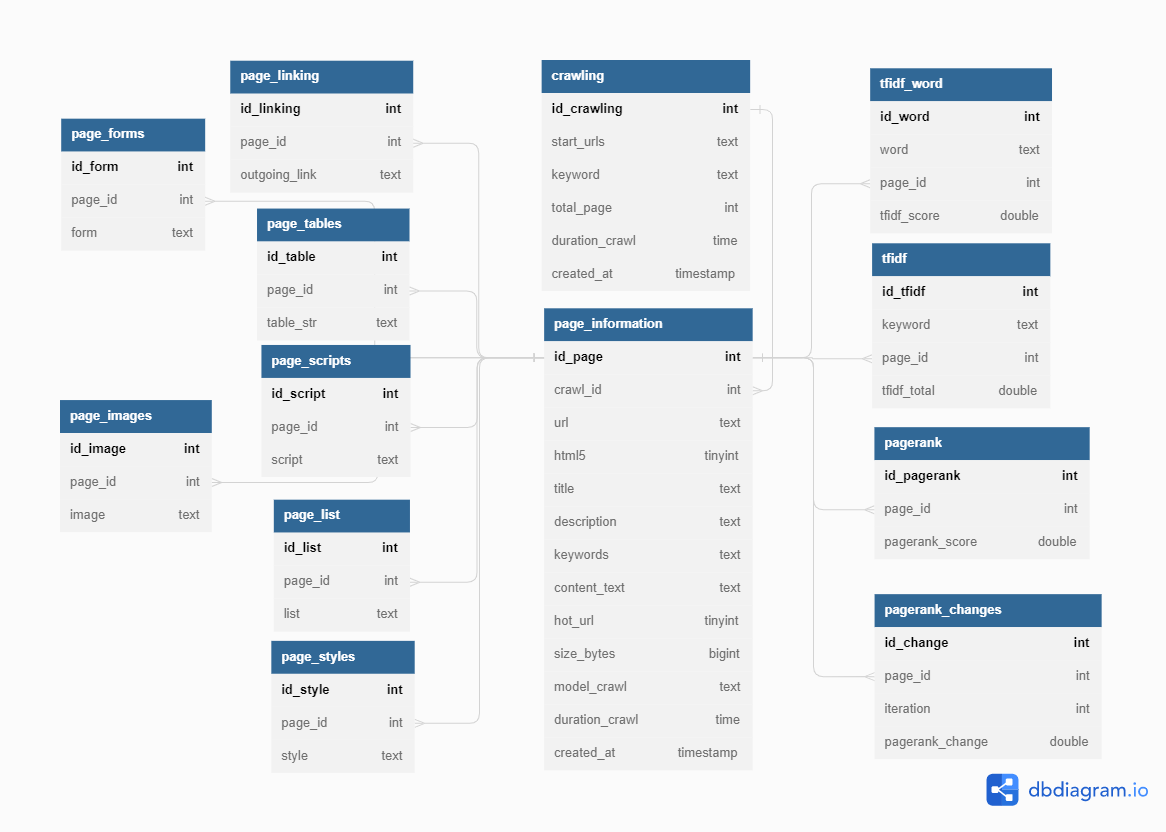
\includegraphics[keepaspectratio, width=12cm]{gambar/ERD Crawler.png}
%		\caption{Skema database yang digunakan dalam proses crawling}}
%	\label{gambar:ERD Crawler.png}
%\end{figure}
%
%Pada saat proses \textit{crawling} berjalan, \textit{crawler} membutuhkan beberapa tabel untuk menyimpan informasi yang didapatkan \textit{crawler} dalam proses berjalannya. Tabel-tabel tersebut diantaranya adalah: \textit{page linking} merupakan tabel untuk menyimpan link keluar dari suatu halaman, \textit{page images} digunakan untuk menyimpan semua gambar yang ada dalam suatu halaman, \textit{page scripts} digunakan untuk menyimpan semua \textit{script} yang terdapat dalam suatu halaman, \textit{page tables} digunakan untuk menyimpan semua tabel yang terdapat pada suatu halaman, \textit{page styles} digunakan untuk menyimpan \textit{style} yang bertugas untuk memberi tampilan pada suatu halaman, \textit{page forms} untuk menyimpan semua form yang terdapat dalam suatu halaman dan \textit{page list} untuk menyimpan seluruh \textit{list} dalam suatu halaman. Masing masing dari tabel yang telah disebutkan terbeut berhubungan \textit{Many to one} dengan tabel \textit{page information}. Sedangkan untuk tabel yang digunakan untuk \textit{document ranking} dan \textit{page ranking} adalah tabel tfidf, tabel tfidf word dan tabel pagerank. Untuk menyimpan informasi awal guna untuk memulai proses crawling digunakan tabel crawling sebagai tempat penyimpanannya. Adapun konsumsi penyimpanan yang dikonsumsi oleh masing masing tabel ditampilkan sebaai berikut. 
%
%
%\begin{figure}[H]
%	{\centering
%		\includegraphics[keepaspectratio, width=12cm]{gambar/db-usage.png}
%		\caption{Penggunaan storage masing masing tabel dalam database}}
%	\label{gambar:db-usage.png}
%\end{figure}


\section{Celery}

Celery merupakan \textit{framework task queue} yang ditulis dengan menggunakan bahasa pemrograman \textit{python}. Program \textit{Celery} dapat membantu menangani tugas tugas yang berkaitan dengan mengatur pembagian kerja dalam beberapa pekerja.


\section{Mongo DB}
MongoDB dikembangkan pada tahun 2007 oleh Eliot dan Dwight untuk 10gen, yang merupakan sistem basis data yang berbasis dokumen yang dapat berjalan di berbagai platform. MongoDB termasuk basis data yang jatuh pada kategori NoSQL. Salah satu alasan dibuatnya MongoDB adalah kemampuan manajemen data dalam jumlah besarnya \citep{mongoarchitecture}.  MongoDB menyimpan dokumen dalam bentuk seperti JSON atau \textit{Javascript Object Annotation} yang bentuknya dapat bermacam macam. Informasi yang relevan dapat disimpan secara bersama sama untuk \textit{query} dengan akses yang cepat dengan \textit{MongoDB query language}. MongoDB menggunakan skema yang dinamis yang membantu dalam membuat \textit{record} tanpa mendefinisikan strukturnya terlebih dahulu seperti atribut atau tipe data. MongoDB memungkinkan untuk mengubah struktur data dengan mudah dengan cara menambahkan atribut atau menghapus atribut yang ada. Model penyimpanan seperti ini membuat membantu dalam merepresentasikan hubungan hierarki, menyimpan data \textit{arrays} dan struktur yang kompleks lainnya dengan mudah. Sebuah dokumen dalam suatu \textit{record} tidak diharuskan memiliki atribut yang sama. MongoDB dirancang untuk availabilitas tinggi dan skalabilitas yang termasuk \textit{replication} dan \textit{auto-sharding} \citep{mongoarchitecture2}.

MongoDB mendukung dua tipe replikasi yaitu \textit{master-slave} dan \textit{replica sets}. Dalam replikasi \textit{master-slave}, \textit{master} mempunyai akses data penuh dan menentukan siapa yang berhak menulis setiap perubahan kepada \textit{slave}. Para \textit{slave} dalam tipe replika ini hanya dapat membaca data saja. Untuk \textit{replica sets}, memiliki cara kerja yang sama dengan replikasi \textit{master-slave}, akan tetapi \textit{replica sets} memungkinkan untuk memilih \textit{master} yang baru jikalau \textit{master} yang lama tidak dapat melakukan kewajibannya. Fitur lainnya yang didukung oleh MongoDB adalah \textit{automatic sharding}. Dengan menggunakan fitur ini, data dapat dibagi-bagi ke beberapa \textit{node}. Seseorang harus memverfikasi \textit{sharding key} untuk setiap \textit{collection} yang mendefiniskan bagaimana suatu dokumen dapat dibagi-bagi. \citep{mongoarchitecture2}

\begin{figure}[H]
	\centering
	\includegraphics[keepaspectratio, width=16cm]{gambar/arsitektur-mongodb}
	\caption{Arsitektur MongoDB}
	\label{gambar:arsitektur-mongodb}
\end{figure}

Pada umumnya dalam arsitektur MongoDB terdapat beberapa komponen pendukung seperti:
\begin{enumerate}
	\item{\emph{Configuration Servers} bertugas untuk menyimpan metadata dari \textit{sharded cluster}. Data yang disimpan mengandung informasi berupa \textit{mapping dataset cluster} dengan \textit{shard}. Komponen seperti \textit{query router} menggunakan data ini untuk menargetkan operasi yang datang ke shard yang sesuai.} 
	\item{\emph{Query Routers}  berhadapan langsung dengan aplikasi dan mengalihkan operasi ke shard atau shards yang sesuai.} 
	\item {\emph{Shards} menyimpan data dan memberikan availabilitas dan konsistensi data yang tinggi.}
\end{enumerate}

Dibandingkan dengan MySQL, MongoDB lebih baik dalam hal pemrosesan query \citep{mongoarchitecture2}. Hal ini dibuktikan dengan penelitian yang bertujuan untuk melihat kelebihan antara penggunaan database non-relasional MongoDB dengan database relasional MySQL. Pada penelitian ini dilakukan beberapa operasi basik kepada kedua database yaitu MongoDB dan MySQL. Operasi yang dilakukan yaitu \textit{insert}, \textit{select}, \textit{update} dan \textit{delete}. Penelitian dilakukan dengan perangkat keras seperti Windows 7
Ultimate 64-bit, prosessor Intel Core i3 (2.4 GHz), 4 GB RAM memory. Sebelum penelitian dilakukan kedua database memiliki beberapa tabel denngan skema yang sama yaitu:

\begin{enumerate}
	\item{tabel/dokumen \textit{User} dengan kolom id, username,
		password, email.}
	\item{tabel/dokumen \textit{Forum} dengan kolom: id, title,
		author, info (short description).}
	\item{tabel/dokumen \textit{Subforum} denga kolom: id, title,
		author, info, created, updated.}
	\item{tabel/dokumen \textit{Discussion} dengan kolom: id, title,
		author, created, updated, content. }
	\item{tabel/dokumen \textit{Comments} dengan kolom: id, author,
		created, content, approved. }
\end{enumerate}

Pemasukan data dimulai dengan memasukan data pengguna ke kedua database, 10.000 pengguna dimasukan ke dalam dua database. Untuk id user dihasilkan secara automatis oleh kedua database dan untuk atribut seberti \textit{username}, \textit{password} dan alamat \textit{email} digunakan fungsi PHP seperti \textit{md5}, \textit{rand}, \textit{substr} dan \textit{str shuffle}. Setelah pemasukan data dilakukan, MySQL memerlukan waktu selama 440 detik sedangkan MongoDB memerlukan waktu sekitar 0.29 detik. Untuk pengujian performa \textit{query} data data dalam jumlah besar, terlihat MongoDB lebih performan daripada MySQL.

\begin{figure}[H]
	\centering
	\includegraphics[keepaspectratio, width=12cm]{gambar/2-grafik-mongomysql-1}
	\caption{Perbandingan performa pemasukan data pengguna untuk kedua database}
	\label{gambar:2-grafik-mongomysql-1}
\end{figure}

Ketika semua pengguna berhasil dimasukan kedalam database, pemasukan data dilanjutkan dengan pemasukan data forum, subforum, diskusi dan komentar. Untuk pengujian, dilakukan pemasukan 5000 baris data untuk setiap tabel forum, subforum, diskusi, dan komentar. Setelah pemasukan data dilakukan, MySQL memerlukan waktu selama 1010 detik sedangkan MongoDB memerlukan waktu sekitar 3.3331 detik. Ketika semua pengguna berhasil dimasukan kedalam database, pemasukan data dilanjutkan dengan pemasukan data forum, subforum, diskusi dan komentar. Untuk pengujian, dilakukan pemasukan 5000 baris data untuk setiap tabel forum, subforum, diskusi, dan komentar. Setelah pemasukan data dilakukan, MySQL memerlukan waktu selama 1010 detik sedangkan MongoDB memerlukan waktu sekitar 3.3331 detik. Untuk pengujian performa untuk pemasukan data dalam jumlah besar, terlihat MongoDB lebih performan daripada MySQL dalam hal memasukan data yang besar.

Selanjutnya adalah pengujian operasi \textit{query}, diadakan dua operasi \textit{query} yaitu:
\begin{enumerate}
	\item {\textit{Query} pertama untuk semua diskusi yang suatu user lakukan dan dengan tanggal yang berbeda dari yang ditentukan.}
	\item {\textit{Query} kedua untuk semua pengguna dari database dan jumlah diskusi yang dimulai oleh setiap user}
\end{enumerate}

\begin{figure}[H]
	\centering
	\includegraphics[keepaspectratio, width=12cm]{gambar/2-grafik-mongomysql-2}
	\caption{MySQL vs MongoDB Select}
	\label{gambar:2-grafik-mongomysql-2}
\end{figure}

Dari tabel diatas, untuk operasi query yang pertama, MySQL memerlukan waktu sekitar 0.0018 detik sedangkan MongoDB berhasil dieksekusi dalam waktu 0.0011 detik dan untuk operasi yang kedua, MySQL memerlukan waktu sekitar 0.6478 detik dan MongoDB memerlukan waktu 0.0052 detik. Untuk pengujian performa untuk query data dalam jumlah besar, terlihat MongoDB lebih performan daripada MySQL dalam hal melakukan operasi \textit{query}.

Selanjutnya adalah pengujian operasi \textit{update} database, ada dua operasi \textit{update} yang digunakan dalam pengujian ini:
\begin{enumerate}
	\item{Mengupdate suatu komen yang ditulis oleh suatu user}
	\item{Mengupdate alamat email suatu pengguna}
\end{enumerate}

\begin{figure}[H]
	\centering
	\includegraphics[keepaspectratio, width=12cm]{gambar/2-grafik-mongomysql-3}
	\caption{MySQL vs MongoDB update}
	\label{gambar:2-grafik-mongomysql-3}
\end{figure}

Untuk operasi update yang pertama, MySQL memerlukan waktu sekitar 0.0987 detik sedangkan dalam MongoDB operasi query update yang pertama dilakukan dalam 0.0428 detik. Untuk pengujian performa untuk update data dalam jumlah besar, terlihat MongoDB lebih performan daripada MySQL dalam hal melakukan operasi \textit{update}.

Selanjutnya dilakukan pengujian untuk operasi \textit{delete}. Ada dua operasi \textit{delete} yang dilakukan untuk pengujian yaitu:
\begin{enumerate}
	\item{Menghapus semua forum yang dibuat oleh suatu user}
	\item {Menghapus semua komentar yang dibuat oleh suatu user.}
\end{enumerate}

\begin{figure}[H]
	\centering
	\includegraphics[keepaspectratio, width=12cm]{gambar/2-grafik-mongomysql-4}
	\caption{MySQL vs MongoDB delete }
	\label{gambar:2-grafik-mongomysql-4}
\end{figure}

Dari gambar \ref{gambar:2-grafik-mongomysql-4}, MySQL memerlukan waktu sekitar 0.3524 detik, sedangka MongoDB memerlukan 0.0028 detik dan operasi yang kedua, MySQL memerlukan waktu 0.8231 detik dan MongoDB memerlukan waktu sekitar 0.0064 detik.

MongoDB memberikan waktu eksekusi operasi yang lebih rendah dibandingkan dengan MySQL dalam 4 operasi biasa yang dimana hal ini adalah hal yang penting ketika sebuah aplikasi diharuskan mendukung ribuan pengguna secara bersama-sama. Maka dari itu dari penelitian yang dilakukan sebelumnya, MongoDB mempunyai performa yang baik dan lebih dipilih dibandingkan MySQL \citep{mongomysqlperfomancediff}.




% Baris ini digunakan untuk membantu dalam melakukan sitasi
% Karena diapit dengan comment, maka baris ini akan diabaikan
% oleh compiler LaTeX.
\begin{comment}
\bibliography{daftar-pustaka}
\end{comment}


%!TEX root = ./template-skripsi.tex
%-------------------------------------------------------------------------------
%                            BAB III
%               			PEMBAHASAN
%-------------------------------------------------------------------------------

\chapter{METODOLOGI PENELITIAN}


\section {Deskripsi Penelitian}

Pada penelitian ini akan merancang tampilan dan aplikasi \textit{web} dengan \textit{admin console} untuk \textit{search engine} yang telah dibuat pada penelitian sebelumnya. Berikut merupakan tahapan-tahapan penelitian yang penulis akan lakukan dalam perancangan aplikasi:


\begin{figure}[H]
	\centering
	\includegraphics[keepaspectratio, width=3cm]{gambar/flowchart.png}
	\caption{Tahapan penelitian}
	\label{gambar:flowchart.png}
\end{figure}


\section {Pengumpulan Data}

Peneliti melakukan studi literatur dengan membaca jurnal-jurnal, penelitian terdahulu dan buku yang berkaitan dengan topik penelitian.

\section {Analisa Kebutuhan Sistem}

Dalam penelitian ini, beberapa perangkat keras yang digunakan untuk menunjang pembuatan sistem adalah sebagai berikut:

\begin{enumerate}
	\item Laptop yang mempunyai CPU Intel Core i5-8250U 1.60 GHz (8 Cores) dengan RAM sebesar 12 GB
	\item Koneksi berbasis Wi-Fi
\end{enumerate}

Perangkat keras yang telah disebutkan sudah memenuhi persyaratan dalam menjalankan perangkat lunak yang akan digunakan seperti:

\begin{enumerate}
	\item Windows 10 64 bit
	\item Visual Studio Code
	\item Figma
	\item Adobe Illustrator CC6
\end{enumerate}

\section {Perancangan Sistem Dengan Scrum}


%Dalam penelitian ini akan digunakan metode \textit{scrum} agar penelitian ini menjadi lebih terstruktur dan mudah. Desain penelitian akan menjelaskan tahapan tahapan yang akan dilakukan penulis dalam penelitian ini dengan menggunakan metode \textit{scrum}.
%
%\begin{figure}[H]
%	\centering
%	\includegraphics[keepaspectratio, width=13cm]{gambar/desain-penelitianpng.png}
%	\caption{Desain Penelitian}
%	\label{gambar:desain-penelitianpng.png}
%\end{figure}

%Tahap pertama yang akan dilakukan pada penelitian ini adalah membuat \textit{product backlog} dari sistem yang akan dibuat, lalu membuat jadwal pengerjaan atau \textit{sprint backlog}. Setelah itu, sprint dimulai dengan diselingi \textit{daily scrum} untuk melaporkan progress dan menentukan task selanjutnya. Setelah sistem selesai dikerjakan di dalam sprint, maka dilakukan pengujian sistem.

Agar penelitian ini menjadi lebih terstruktur dan mudah, maka penelitian ini akan menggunakan metode \textit{scrum} sebagai metode pengembangan sistemnya. Berdasarkan gambar \ref{gambar:desain-penelitianpng.png}, komponen-komponen \textit{scrum} terdiri dari \textit{product backlog}, \textit{sprint backlog}, \textit{daily scrum} dan \textit{sprint} lalu dilanjutkan dengan pengujian sistem yang sudah dibuat.


\begin{figure}[H]
	\centering
	\includegraphics[keepaspectratio, width=13cm]{gambar/desain-penelitianpng.png}
	\caption{Tahapan penelitian dengan menggunakan metode \textit{scrum}}
	\label{gambar:desain-penelitianpng.png}
\end{figure}

\begin{enumerate}
	\item \textit{Product backlog}

	\textit{Product backlog} merupakan kumpulan tugas yang akan dilaksanakan. \textit{Product backlog} seperti ditunjukan oleh tabel \ref{productbacklog} penelitian ini terdiri dari 3 komponen yaitu \textit{story}, \textit{sprint} dan \textit{status}. \textit{Story} ialah sebuah pekerjaan besar yang dapat dibagi bagi lebih kecil lagi menjadi tugas tugas kecil. \textit{Sprint} menandakan \textit{sprint} berapa \textit{story} tersebut akan diselesaikan. \textit{Status} memberitahu apakah \textit{sprint} tersebut sudah terlaksanakan atau belum.
	
	\begin{table}[H]
		\centering
		\caption{\textit{Product Backlog}}
		\label{productbacklog}
		\begin{tabular}{@{} |p{1cm}|p{7cm}| p{1cm} |p{2.5cm}|@{}}
			\hline
			\textbf{No.} & \textbf{\textit{Story}} & \textbf{\textit{Sprint}} & \textbf{\textit{Status}} \\
			\hline
			1 & Fitur pencarian pengguna & 1, 2, 8 & Selesai \\
			\hline
			2 & Fitur \textit{page ranking} & 4, 5 & Selesai\\
			\hline
			3 & Fitur \textit{staff} & 5, 8 & Selesai\\
			\hline
			4 & Fitur \textit{document ranking} & 5, 7  & Selesai\\
			\hline
			5 & Fitur \textit{crawling} & 3, 6 & Selesai\\
			\hline
			6 & Struktur projek & 2 & Selesai\\
			\hline
			7 & \textit{multi-threaded service} & 10  & Selesai\\
			\hline
			8 & \textit{Service deployment} & 11  & Selesai\\
			\hline
			9 & Background task dengan \textit{Celery} & 12  & Selesai\\
			\hline
			10 & Pengujian penggunaan memori & 13  & Selesai\\
			\hline
		\end{tabular}
	\end{table}

	\item{Sprint Backlog}
	
	\textit{Sprint backlog} merupakan daftar tugas tugas kecil yang perlu dilaksanakan pada suatu \textit{sprint}.
	
	\item{Sprint}
	
	\textit{Sprint} merupakan masa dimana pengerjaan tugas tugas yang telah direncanakan pada suatu \textit{sprint} dilakukan. Lama durasi setiap \textit{sprint} ditentukan oleh \textit{scrum master} yang telah disepakati bersama.
	
	\item{Daily Scrum}
	
	\textit{Daily scrum} merupakan pertemuan dengan \textit{scrum master} untuk membahas tugas apa yang telah dicapai hari kemarin dan tugas apa yang ingin dicapai hari ini yang dilaksanakan setiap hari.
\end{enumerate}

% Tahapan pertama yang dilakukan pada penelitian ini adalah mendefinisikan sebuah \textit{product backlog} penelitian dan mendifinisikan \textit{sprint backlog} yang merupakan jadwal pengerjaan tugas tugas yang akan dibuat. Setelah kedua komponen tersebut berhasil dibuat, maka \textit{sprint} dapat dimulai dari awal dengan diselingi \textit{daily scrum} untuk melakukan pelaporan \textit{progress} penelitian yang sedang dilakukan. Berikut ini adalah tabel \textit{product backlog} yang telah dibuat. 


%
%
%Berdasarkan tabel \ref{productbacklog}, \textit{product backlog} penelitian ini terdiri dari 3 komponen yaitu \textit{story}, \textit{sprint} dan \textit{status}. \textit{Story} ialah sebuah pekerjaan besar yang dapat dibagi bagi lebih kecil lagi menjadi tugas tugas kecil. \textit{Sprint} menandakan \textit{sprint} berapa \textit{story} tersebut akan diselesaikan. \textit{Status} memberitahu apakah \textit{sprint} tersebut sudah terlaksanakan atau belum.
%
%\section{\textit{Sprint} 1}
%
%\begin{table}[H]
%	\centering
%	\caption{\textit{Sprint-1 Backlog}}
%	\label{uat}
%	\begin{tabular}{@{} |p{1cm}|p{3cm}| p{6cm} |p{2.5cm}|@{}}
	%		\hline
	%		\textbf{No.} & \textbf{\textit{Story}} & \textbf{\textit{Task}} & \textbf{\textit{Status}} \\
	%		\hline
	%		1 & Membuat rancangan tampilan dashboard \textit{search engine} & \begin{enumerate}
		%			\item Penentuan desain sistem
		%			\item Perancangan desain halaman kelola admin
		%			\item Perancangan desain halaman \textit{page rank matrix}
		%			\item Perancangan desain halaman peta situs admin
		%			\item Perancangan desain halaman pencarian pengguna
		%			\item Perancangan desain halaman peta situs pengguna
		%			\item Perancangan desain halaman hasil pencarian pengguna
		%			\item Perancangan desain halaman ranking situs			
		%			\item Pendataan route table yang sudah ada dengan tampilan yang ada
		%			\item Desain route table untuk web service yang belum ada
		%		\end{enumerate} & \\
	%		\hline
	%		
	%	\end{tabular}
%\end{table}
%Pada \textit{sprint} ini akan dilakukan perancangan tampilan untuk \textit{search engine} ONE (\textit{Omniscience Network Extractor}) dilakukan dengan perangkat lunak Figma dan Adobe Illustrator. Untuk memudahkan proses dalam perancangan tampilan untuk \textit{search engine} yang akan dibangun, diperlukan adanya suatu sistem desain untuk \textit{sizing}, \textit{spacing} dan \textit{color} atau warna.
%
%Dalam sistem desain untuk \textit{spacing} dan \textit{sizing} digunakan seperti tabel berikut
%
%\begin{table}[H]
%	\caption{\textit{Sistem desain \textit{sizing} dan \textit{spacing}}}
%	\label{Sistem desain sizing dan spacing}
%	\includegraphics[keepaspectratio, width=13cm]{gambar/g-109.png}
%\end{table}
%
%Untuk sistem desain warna, warna biru \textit{navy} digunakan sebagai warna utama tampilan \textit{search engine}. Adapun \textit{shades} dari warna utama yaitu \textit{navy} adalah sebagai berikut. Warna \textit{shades} ditentukan dengan cara mengatur nilai \textit{hue}, \textit{saturation} dan \textit{lightning} dari warna utama.
%
%
%\begin{figure}[H]
%	\centering
%	\includegraphics[keepaspectratio, width=13cm]{gambar/g-110.png}
%	\caption{Desain Penelitian}
%	\label{gambar:g-110.png}
%\end{figure}
%
%Hal pertama yang dilakukan dalam pembuatan tampilan dari \textit{search engine} adalah mendesain sebuah logo. Sebuah logo digunakan sebagai identitas bagi \textit{search engine} yang akan dibuat tentulah harus mempunyai makna. Logo yang akan dibuat berbentuk "O" melambangkan huruf pertama dari nama search engine tersebut yaitu "ONE". Tanpa warna, logo pola jaring akan terlihat dalam lingkaran berbentuk O yang melambangkan suatu hubungan dari banyaknya sebuah situs. Untuk pewarnaan, digunakan warna oranye yang melambangkan huruf O dari nama \textit{search engine} tersebut, warna \textit{navy} melambangkan huruf N dari nama \textit{search engine} dan warna \textit{eclipse} melambangkan huruf terakhir dari \textit{search engine} tersebut yaitu E.
%
%
%\begin{figure}[H]
%	\centering
%	\includegraphics[keepaspectratio, width=13cm]{gambar/g-111.png}
%	\caption{Desain Logo ONE \textit{Search Engine}}
%	\label{gambar:g-111.png}
%\end{figure}
%
%\begin{figure}[H]
%	\centering
%	\includegraphics[keepaspectratio, width=13cm]{gambar/g-113.png}
%	\caption{Desain sistem warna pada logo ONE}
%	\label{gambar:g-113.png}
%\end{figure}
%%
%%Penelitian ini akan menggunakan data yang berasal dari penelitian \citep{lazu} yang digunakan berasal dari proses \textit{crawling} yang dilakukan sebelumnya. Pada penelitian \citep{lazu} telah dibuat aplikasi berbasis flask untuk menyediakan cara yang mudah bagi tampilan aplikasi untuk berkomunikasi dengan data yang telah disediakan. Untuk menghubungkan data dari penelitian yang telah disediakan dengan tampilan yang akan dibuat digunakan sebuah \textit{Application Programming Interface} yang memenuhi arsitektur desain perangkat lunak {Representational State Transfer} atau biasa disebut dengan \textit{Rest API}. Adapun skema {Rest API} yang telah dibuat oleh \citep{lazu} adalah sebagai berikut.
%%
%%\begin{table}[H]
%%	\caption{\textit{Routing table REST API}}
%%	\label{routing_table}
%%	\includegraphics[keepaspectratio, width=13cm]{gambar/routing_table}
%%\end{table}
%%
%%Terdapat tambahan \textit{Routing} guna untuk memenuhi fitur yang akan dibangun yaitu
%%
%%
%%\begin{table}[H]
%%	\centering
%%	\caption{\textit{Routing Table Tambahan}}
%%	\label{uat}
%%	\begin{tabular}{@{} |p{1cm}|p{5cm}| p{2cm}|p{2cm}|p{2cm}|p{2cm} |p{2cm}|@{}}
	%%		\hline
	%%		\textbf{Name} & \textbf{\textit{Route}} & \textbf{\textit{Method}} & \textbf{\textit{Description}}  & \textbf{\textit{Body}} & \textbf{\textit{Query}} \\
	%%		\hline
	%%		1 & /api/v1/domains & GET & Mendapatkan daftar domain yang berhasil di crawl & - & page, limit, countries, query \\
	%%		\hline
	%%		2 & /api/v1/metrics & GET & Mendapatkan statistik \textit{crawler} &   & - \\
	%%		\hline
	%%		3 & /api/v1/admins & GET & Mendapatkan daftar admin \textit{crawler} & -  &  page, limit, roles, query \\
	%%		\hline
	%%		4 & /api/v1/admins/:id/delete & DELETE & Menghapus admin & -  &  - \\
	%%		\hline
	%%		5 & /api/v1/admins/:id/update & PATCH & Mengupdate admin & firstName, lastName, username, role, status, email, profilePictureUrl  &  - \\
	%%		\hline
	%%		6 & /api/v1/admins/:id & GET & Mendapatkan data admin & - &  - \\
	%%		\hline
	%%		7  & /api/v1/login & POST & Login admin & - & - \\
	%%		\hline
	%%	\end{tabular}
%%\end{table}
%%
%%
%%Dari tabel \textit{REST API} diatas dan analisa database yang telah dilakukan sebelumnya, akan dilakukan pembuatan desain tampilan untuk \textit{search engine}. 
%
%Terdapat dua bagian dari tampilan \textit{search engine}, yaitu bagian untuk admin untuk manajemen \textit{search engine} dan tampilan untuk \textit{pengguna}.
%
%\subsection{Penentuan \textit{Font}}
%
%Menurut \citep{refactoringui}, jenis font dapat ditentukan dengan observasi jenis \textit{font} yang digunakan dari aplikasi lain yang sudah ada di pasaran. Pada dasarnya, aplikasi yang sudah ada di pasasran memiliki beberapa orang perancang yang memiliki pengalaman lebih mengenai \textit{typography} untuk menentukan jenis \textit{font} yang akan mereka gunakan biasanya dengan telah memperhitungkan berbagai faktor. Setelah melakukan observasi pada aplikasi besar yang ada pada pasaran, peneliti memutuskan untuk menggunakan \textit{font} \textit{Inter} sebagai jenis \textit{font} utama pada aplikasi dikarenakan jenis \textit{font} ini sudah banyak sekali digunakan pada aplikasi besar yang terdapat di pasaran dan bersifat \textit{open source}.
%
%\subsection{Penentuan \textit{White Spacing} Komponen}
%
%Dalam penentuan \textit{white spacing} dari setiap komponen yang akan dibuat, penulis menggunakan metode \textit{decremental} seperti yang telah dibahas sebelumnya. Pemberian \textit{white spacing} secara \textit{decremental} adalah sebuah cara untuk menemukan nilai \textit{white spacing} yang cocok digunakan pada komponen yang akan dibuat dengan cara memberikan nilai awal \textit{white spacing} yang besar kepada komponen yang akan dibuat dan mengurangi nilai \textit{white spacing}-nya secara bertahap sampai dapat dikatakan cocok. Dalam pemberian \textit{white spacing} penulis menggunakan sistem desain \textit{white spacing} dan \textit{sizing} yang telah ditentukan sebelumnya.
%
%
%\begin{figure}[H]
%	\centering
%	\includegraphics[keepaspectratio, width=13cm]{gambar/example-whitespace-decremental-1.png}
%	\caption{Pemberian nilai \textit{white spacing} awal yang besar terhadap komponen \textit{button}}
%	\label{gambar:example-whitespace-decremental-1.png}
%\end{figure}
%
%
%\begin{figure}[H]
%	\centering
%	\includegraphics[keepaspectratio, width=13cm]{gambar/example-whitespace-decremental-2.png}
%	\caption{Pemberian nilai \textit{white spacing} secara \textit{decremental} terhadap komponen \textit{button} sehingga \textit{white spacing} yang diberikan terasa cocok}
%	\label{gambar:example-whitespace-decremental-2.png}
%\end{figure}
%
%
%
%\subsection{Halaman \textit{Dashboard} Admin}
%
%Pada desain halaman dashboard untuk admin yang telah dibuat, terdapat bagian \textit{search engine metrics}. Pada bagian ini terdapat informasi dari \textit{search engine} seperti korelasi \textit{pagerank}, total \textit{assets} yang berhasil di-\textit{crawl}, statistik url yang telah di-\textit{crawl}, total jumlah url yang telah di-\textit{crawl} dan jumlah kata yang telah di-\textit{crawl}. Pada halaman ini juga terdapat tabel yang dapat digunakan untuk mengelola semua url yang telah di-\textit{crawl}. Pada halaman ini jarak antara komponen dalam halaman dibuat lebih kecil guna untuk memuat informasi dalam jumlah banyak dalam satu halaman \citep{refactoringui}. Pada tombol ini terdapat tombol pagerank matrix yang berguna untuk menavigasi admin ke halaman \textit{pagerank matrix}.
%
%\begin{figure}[H]
%	\centering
% 	\includegraphics[keepaspectratio, width=13cm]{gambar/g-114.png}
%	\caption{Desain tampilan dashboard \textit{search engine}}
%	\label{gambar:dashboard.png}
%\end{figure}
%
%Adapun routing tabel dari halaman ini adalah sebagai berikut
%
%
%\begin{table}[H]
%	\centering
%	\caption{\textit{Routing Table Halaman Dashboard Admin}}
%	\label{uat}
%	\begin{tabular}{@{} |p{0.5cm}|p{3.5cm}| p{1.5cm}|p{2cm}|p{2cm}|p{2cm} |p{2cm}|p{0.5cm}|@{}}
	%		\hline
	%		\textbf{No.} & \textbf{\textit{Route}} & \textbf{\textit{Method}} & \textbf{\textit{Description}}  & \textbf{\textit{Body}} & \textbf{\textit{Query}} &  \textbf{\textit{Return}} \\
	%		\hline
	%		1 & /api/v1/domains & GET & Mendapatkan daftar domain yang berhasil di crawl & - & page, limit, countries, query & JSON \\
	%		\hline
	%		2 & /api/v1/metrics & GET & Mendapatkan statistik dashboard &   & -  & JSON \\
	%		\hline
	%		3 & /api/v1/domains/:id /delete & DELETE & Menghapus suatu domain & - & - & JSON \\
	%		\hline
	%		4 & /dashboard & GET & Menampilkan halaman dashboard & - & -  & View \\
	%		\hline
	%	\end{tabular}
%\end{table}
%
%\subsection{Halaman \textit{Page Rank Matrix}}
%
%Pada halaman \textit{page rank matrix} admin dapat melihat nilai \textit{page rank matrix} per-domain atau seluruh domain. Pembuatan halaman ini bertujuan agar memudahkan sisi admin dalam melihat \textit{page rank matrix} dari suatu domain ataupun seluruh domain yang berhasil di-\textit{crawl}. Halaman ini tersedia dalam bentuk tiga dimensi dan dua dimensi. Pembuatan halaman ini dalam graf tiga dimensi bertujuan untuk mempermudah pengguna dalam melihat \textit{domain} yang direpresentasikan dengan titik dan garis yang merepresentasikan \textit{outgoing} link dari setiap domain yang ada.
%
%
%\begin{figure}[H]
%	\centering
%	\includegraphics[keepaspectratio, width=13cm]{gambar/page_rank_matrix_visualizer.png}
%	\caption{Desain tampilan \textit{page rank matrix} per-domain atau seluruh domain dalam bentuk dua dimensi}
%	\label{gambar:page_rank_matrix_visualizer.png}
%\end{figure}
%
%\begin{figure}[H]
%	\centering
%	\includegraphics[keepaspectratio, width=13cm]{gambar/pagerank-matrix-3d.png}
%	\caption{Desain tampilan \textit{page rank matrix} per-domain atau seluruh domain dalam bentuk tiga dimensi}
%	\label{gambar:pagerank_matrix_3d.png}
%\end{figure}
%
%
%Adapun routing tabel dari halaman ini adalah sebagai berikut
%
%
%\begin{table}[H]
%	\centering
%	\caption{\textit{Routing Table Halaman Dashboard Admin}}
%	\label{uat}
%	\begin{tabular}{@{} |p{0.5cm}|p{3.5cm}| p{1.5cm}|p{2cm}|p{2cm}|p{2cm} |p{2cm}|p{0.5cm}|@{}}
	%		\hline
	%		\textbf{No.} & \textbf{\textit{Route}} & \textbf{\textit{Method}} & \textbf{\textit{Description}}  & \textbf{\textit{Body}} & \textbf{\textit{Query}} &  \textbf{\textit{Return}} \\
	%		\hline
	%		1 & /pagerank-matrix & GET & Menampilkan halaman matrix dari suatu atau seluruh domain dalam bentuk 2 dimensi atau 3 dimensi & - & type, domain & View \\
	%		\hline
	%	\end{tabular}
%\end{table}
%
%
%\subsection{Halaman Kelola Admin}
%
%Pada halaman kelola admin untuk admin berfokus pada pengelolaan admin pada \textit{search engine} yang telah dibuat. Terdapat beberapa fitur seperti \textit{update} admin, tambah admin, list admin dan pencarian admin. Desain tampilan dibuat seperti daftar berguna untuk memudahkan pengguna dalam menavigasi dari satu admin ke admin yang lainnya.  Halaman ini dibuat tidak memenuhi semua \textit{white spacing} yang tersedia bertujuan agar pengguna lebih mudah dalam menginterpretasikan maksud dan fungsi dari halaman yang sedang dibuka.
%
%\begin{figure}[H]
%	\centering
%	\includegraphics[keepaspectratio, width=13cm]{gambar/managa_admin.png}
%	\caption{Desain tampilan kelola admin \textit{search engine}}
%	\label{gambar:managa_admin.png}
%\end{figure}
%
%Pada tombol tambah admin, admin akan dinavigasikan ke halaman formulir tambah admin.
%
%\begin{figure}[H]
%	\centering
%	\includegraphics[width=16cm]{gambar/add-admin.png}
%	\caption{Desain tampilan update admin \textit{search engine}}
%	\label{gambar:add-admin.png}
%\end{figure}
%
%Untuk tombol update pada halaman kelola admin, admin akan dinavigasikan ke halaman update admin guna mengupdate informasi mengenai admin.
%
%\begin{figure}[H]
%	\centering
%	\includegraphics[keepaspectratio, width=13cm]{gambar/login-admin.png}
%	\caption{Desain tampilan update admin \textit{search engine}}
%	\label{gambar:login-admin.png}
%\end{figure}
%
%
%Adapun routing tabel dari halaman ini adalah sebagai berikut
%
%
%\begin{longtable}{@{} |p{0.5cm}|p{3.5cm}| p{1.5cm}|p{2cm}|p{2cm}|p{2cm} |p{2cm}|p{0.5cm}|@{}}
%	\caption{\textit{Routing Table Halaman Dashboard Admin}}\\
%	\hline
%	\textbf{No.} & \textbf{\textit{Route}} & \textbf{\textit{Method}} & \textbf{\textit{Description}}  & \textbf{\textit{Body}} & \textbf{\textit{Query}} &  \textbf{\textit{Return}} \\
%	\hline
%	1 & /api/v1/admins & GET & Mendapatkan daftar admin \textit{crawler} & -  &  page, limit, roles, query& JSON \\
%	\hline
%	2 & /api/v1/admins/:id /delete & DELETE & Menghapus admin & -  &  -&JSON \\
%	\hline
%	3 & /api/v1/admins/:id /update & PATCH & Mengupdate admin & firstName, lastName, username, role, status, email, profilePictureUrl  &  - &JSON \\
%	\hline
%	4 & /api/v1/admins/:id & GET & Mendapatkan data admin & - &  - & JSON \\
%	\hline
%	5 & /api/v1/admins/:id /create & POST & Menambahkan admin & firstName, lastName, username, role, status, email, profilePictureUrl  &  - &JSON \\
%	\hline
%	6 & /dashboard/admins & GET & Menampilkan halaman kelola & - &  - & View \\
%	\hline
%	7 & /dashboard/admins
%	/add & GET & Menampilkan form tambah admin & - &  - & View \\
%	\hline
%	8 & /dashboard/admins
%	/:id/update & GET & Menampilkan form update admin & - &  - & View \\
%	\hline
%\end{longtable}
%
%
%\subsection{Halaman Peta Situs Admin}
%
%Pada halaman peta situs untuk admin, admin dapat melihat semua situs yang berhasil di-\textit{crawling} dalam bentuk graf 3 dimensi. Graf 3 dimensi dipilih agar visualisasi dari semua link terlihat menarik dan mudah untuk dinavigasi oleh pengguna. Titik dari graf ini adalah sebuah situs dan sisi dari grafnya adalah \textit{outgoing link}. Admin juga dapat mengelola \textit{outgoing link} dari sebuah situs dalam halaman ini. Halaman dibuat dalam tema gelap bertujuan untuk menciptakan suasana luar angkasa dengan titik dari graf melambangkan planet planet yang ada di luar angkasa. Halaman ini dapat diakses dengan menekan tombol "\textit{3D Graph}" pada navigasi \textit{header} yang terdapat di atas halaman web.
%
%\begin{figure}[H]
%	\centering
%	\includegraphics[keepaspectratio, width=13cm]{gambar/admin-sitemap.png}
%	\caption{Desain tampilan peta situs untuk admin \textit{search engine}}
%	\label{gambar:admin-sitemap.png}
%\end{figure}
%
%
%Adapun routing tabel dari halaman ini adalah sebagai berikut
%
%\begin{longtable}{@{} |p{0.5cm}|p{3.5cm}| p{1.5cm}|p{2cm}|p{2cm}|p{2cm} |p{2cm}|p{0.5cm}|@{}}
%	
%	\caption{\textit{Routing Table Halaman Peta Situs Admin}}\\
%	\hline
%	\textbf{No.} & \textbf{\textit{Route}} & \textbf{\textit{Method}} & \textbf{\textit{Description}}  & \textbf{\textit{Body}} & \textbf{\textit{Query}} &  \textbf{\textit{Return}} \\
%	\hline
%	1 & /api/v1/sites/:id
%	/delete & DELETE & Mendelete suatu situs & -  & - & JSON \\
%	\hline
%	2 & /api/v1/sites/:id
%	/update & UPDATE & Mengupdate suatu situs & title, link  & - & JSON \\\hline
%	3 & /api/v1/sites/:id
%	/outgoing & GET & Mendapatkan semua situs outgoing dari suatu situs & -  & limit, page & JSON \\
%	\hline
%	4 & /api/v1/sites/:id & GET & Mendapatkan informasi dari suatu situs & - & - & JSON \\\hline
%	5 & /dashboard/sitemap & GET & Menampilkan halaman peta situs untuk admin & - & site, mode & View \\
%	\hline
%	\hline
%\end{longtable}
%
%
%\subsection{Halaman Login Admin}
%
%Pada halaman login admin, admin dapat login ke dalam \textit{dashboard} admin dengan menggunakan \textit{email} dan password yang telah disediakan. Halaman \textit{login} dibuat menengah agar mata pengguna hanya fokus ke bagian tengah saja dan membuat pengguna lebih mudah menginterpretasikan maksud dan fungsi dari halaman yang sedang dibuka.
%
%\begin{figure}[H]
%	\centering
%	\includegraphics[keepaspectratio, width=13cm]{gambar/admin-login-page.png}
%	\caption{Desain tampilan \textit{login} admin \textit{search engine}}
%	\label{gambar:admin-login-page.png}
%\end{figure}
%
%
%\begin{table}[H]
%	\centering
%	\caption{\textit{Routing Table Halaman Dashboard Admin}}
%	\label{uat}
%	\begin{tabular}{@{} |p{0.5cm}|p{3.5cm}| p{1.5cm}|p{2cm}|p{2cm}|p{2cm} |p{2cm}|p{0.5cm}|@{}}
	%		\hline
	%		\textbf{No.} & \textbf{\textit{Route}} & \textbf{\textit{Method}} & \textbf{\textit{Description}}  & \textbf{\textit{Body}} & \textbf{\textit{Query}} &  \textbf{\textit{Return}} \\
	%		\hline
	%		1 & /api/v1/login & GET & Mendapatkan daftar admin \textit{crawler} & email, password  & - & JSON \\ \hline
	%		2 & /dashboard/login & POST & Menampilkan halaman login dashboard untuk admin & - & - & View \\
	%		\hline
	%	\end{tabular}
%\end{table}
%
%\subsection{Halaman Pencarian Pengguna}
%
%Pada halaman pencarian untuk pengguna, pengguna dapat melakukan pencarian pada halaman ini. Terdapat dua menu pada bagian \textit{header} yang dapat pengguna akses yaitu ranking situs dan peta web. Pada halaman ini juga disediakan pencarian pengguna sebelumnya. Bagian \textit{recent searches} betujuan untuk memudahkan pengguna dalam mencari kata pencarian yang pernah dicari sebelumnya. Halaman ini dibuat tidak memenuhi \textit{white spacing} yang tersedia bertujuan agar pengguna lebih mudah dalam menginterpretasikan maksud dan fungsi dari halaman yang sedang dibuka.  Halaman ini dibuat tidak memenuhi semua \textit{white spacing} yang tersedia bertujuan agar pengguna lebih mudah dalam menginterpretasikan maksud dan fungsi dari halaman yang sedang dibuka.
%
%\begin{figure}[H]
%	\centering
%	\includegraphics[keepaspectratio, width=13cm]{gambar/user-search-page.png}
%	\caption{Desain tampilan halaman pencarian untuk pengguna}
%	\label{gambar:user-search-page.png}
%\end{figure}
%
%
%\begin{table}[H]
%	\centering
%	\caption{\textit{Routing Table Halaman Pencarian Pengguna}}
%	\label{uat}
%	\begin{tabular}{@{} |p{0.5cm}|p{3.5cm}| p{1.5cm}|p{2cm}|p{2cm}|p{2cm} |p{2cm}|p{0.5cm}|@{}}
	%		\hline
	%		\textbf{No.} & \textbf{\textit{Route}} & \textbf{\textit{Method}} & \textbf{\textit{Description}}  & \textbf{\textit{Body}} & \textbf{\textit{Query}} &  \textbf{\textit{Return}} \\
	%		\hline
	%		1 & /api/v1/search & GET & Mendapatkan daftar admin \textit{crawler} & - & - & query \\ \hline
	%		2 & / & GET & Menapilkan halaman pencarian untuk pengguna & - & - & View \\
	%		\hline
	%	\end{tabular}
%\end{table}
%
%\subsection{Halaman Peta Situs Pengguna}
%
%Sama seperti peta situs untuk admin, pengguna dapat melihat semua situs yang berhasil di-\textit{crawling} dalam bentuk graf 3 dimensi. Graf 3 dimensi dipilih agar visualisasi dari semua link terlihat menarik dan mudah untuk dinavigasi oleh pengguna. Titik dari graf ini adalah sebuah situs dan sisi dari grafnya adalah \textit{outgoing link}. Pengguna dapat melihat \textit{outgoing link} dari sebuah situs yang difokuskan pada bagian kanan layar. Pengguna juga dapat memfokuskan \textit{link} yang lain dengan menekan salah satu dari titik titik yang ada. Halaman dibuat dalam tema gelap bertujuan untuk menciptakan suasana luar angkasa dengan titik dari graf melambangkan planet planet yang ada di luar angkasa.
%
%\begin{figure}[H]
%	\centering
%	\includegraphics[keepaspectratio, width=13cm]{gambar/user-sitemap.png}
%	\caption{Desain tampilan peta situs untuk pengguna \textit{search engine}}
%	\label{gambar:user-sitemap.png}
%\end{figure}
%
%
%Adapun routing tabel dari halaman ini adalah sebagai berikut
%
%\begin{table}[H]
%	\centering
%	\caption{\textit{Routing Table Halaman Peta Situs Pengguna}}
%	\label{uat}
%	\begin{tabular}{@{} |p{0.5cm}|p{3.5cm}| p{1.5cm}|p{2cm}|p{2cm}|p{2cm} |p{2cm}|p{0.5cm}|@{}}
	%		\hline
	%		\textbf{No.} & \textbf{\textit{Route}} & \textbf{\textit{Method}} & \textbf{\textit{Description}}  & \textbf{\textit{Body}} & \textbf{\textit{Query}} &  \textbf{\textit{Return}} \\
	%		\hline
	%		1 & /api/v1/sites/:id
	%		/outgoing & GET & Mendapatkan semua situs outgoing dari suatu situs & -  & limit, page & JSON \\
	%		\hline
	%		2 & /api/v1/sites/:id & GET & Mendapatkan informasi dari suatu situs & - & - & JSON \\\hline
	%		3 & /sitemap & GET & Menampilkan halaman peta situs untuk pengguna  & - & site, mode & View \\
	%		\hline
	%	\end{tabular}
%\end{table}
%
%\subsection{Halaman Hasil Pencarian Pengguna}
%
%Halaman ini merupakan halaman setelah pengguna mamasukan kata pencarian pada \textit{search engine}. Pada halaman ini menyajikan situs-situs yang relevan berdasarkan kata pencarian yang pengguna berikan. Pengguna juga dapat menambahkan parameter tambahan seperti \textit{sort by} dan sebuah \textit{filter} untuk membuat hasil pencarian lebih akurat untuk pengguna. Hasil pencarian dibuat tidak mengisi seluruh \textit{white space} agar pengguna lebih mudah menavigasi hasil pencarian dengan mengurangi pergerakan mata pengguna. Pada hasil pencarian juga disediakan tombol tanda panah miring bertujuan untuk mengantarkan pengguna ke halaman peta situs dan melihat situs hasil pencarian tersebut dalam  bentuk tiga dimensi. Halaman ini dibuat tidak memenuhi semua \textit{white spacing} yang tersedia bertujuan agar pengguna lebih mudah dalam menginterpretasikan maksud dan fungsi dari halaman yang sedang dibuka.
%
%\begin{figure}[H]
%	\centering
%	\includegraphics[keepaspectratio, width=10cm]{gambar/user-search-result.png}
%	\caption{esain tampilan halaman hasil pencarian}
%	\label{gambar:user-search-result.png}
%\end{figure}
%
%
%Adapun routing tabel dari halaman ini adalah sebagai berikut
%
%\begin{longtable}{@{} |p{0.5cm}|p{3.5cm}| p{1.5cm}|p{2cm}|p{2cm}|p{2cm} |p{2cm}|p{0.5cm}|@{}}
%	
%	\caption{\textit{Routing Table Halaman Hasil Pencarian Pengguna}}\\
%	\hline
%	\textbf{No.} & \textbf{\textit{Route}} & \textbf{\textit{Method}} & \textbf{\textit{Description}}  & \textbf{\textit{Body}} & \textbf{\textit{Query}} &  \textbf{\textit{Return}} \\
%	\hline
%	1 & /api/v1/search
%	/outgoing & GET & Mendapatkan semua situs yang terkait dengan kata kunci yang diberikan & -  & limit, page, query, filters, sort & JSON \\
%	\hline
%	2 & /search & GET & Menampilkan halaman hasil pencarian berdasarkan kata kunci yang diberikan & - & limit, page, query, filters, sort & View \\\hline
%\end{longtable}
%
%
%\subsection{Halaman Ranking Situs}
%
%Pada halaman ini akan menampilkan ranking dari semua url yang berhasil di-\textit{crawl}. Halaman perankingan situs dibuat tidak mengisi seluruh \textit{white space} agar pengguna lebih mudah menavigasi ranking situs dengan mengurangi pergerakan mata pengguna. Pada ranking juga disediakan tombol tanda panah miring bertujuan untuk mengantarkan pengguna ke halaman peta situs dan melihat situs hasil pencarian tersebut dalam  bentuk tiga dimensi. Halaman ini dibuat tidak memenuhi \textit{white spacing} yang tersedia bertujuan agar pengguna lebih mudah dalam menginterpretasikan maksud dan fungsi dari halaman yang sedang dibuka.
%
%\begin{figure}[H]
%	\centering
%	\includegraphics[keepaspectratio, width=13cm]{gambar/user-page-ranking-page.png}
%	\caption{Desain tampilan ranking halaman}
%	\label{gambar:user-page-ranking-page.png}
%\end{figure}
%
%
%
%Adapun routing tabel dari halaman ini adalah sebagai berikut
%
%\begin{table}[H]
%	\centering
%	\caption{\textit{Routing Table Halaman Peta Situs Pengguna}}
%	\label{uat}
%	\begin{tabular}{@{} |p{0.5cm}|p{3.5cm}| p{1.5cm}|p{2cm}|p{2cm}|p{2cm} |p{2cm}|p{0.5cm}|@{}}
	%		\hline
	%		\textbf{No.} & \textbf{\textit{Route}} & \textbf{\textit{Method}} & \textbf{\textit{Description}}  & \textbf{\textit{Body}} & \textbf{\textit{Query}} &  \textbf{\textit{Return}} \\
	%		\hline
	%		1 & /api/v1/ranking
	%		/outgoing & GET & Mendapatkan ranking dari semua situs  & -  & limit, page & JSON \\
	%		\hline
	%		2 & /ranking  & GET & Menampilkan halaman ranking situs & - & limit, page, query, filters, sort & View \\\hline
	%	\end{tabular}
%\end{table}


%
%Pada penelitian ini akan digunakan algoritma \textit{page ranking} DPC yang telah dikembangkan oleh \citep{farhan} menggantikan algoritma \textit{PageRank} yang digunakan oleh \citep{lazu}. Penggantian algoritma untuk \textit{PageRank} ini dimulai dengan mengumpulkan informasi berupa fungsi yang bertanggung jawab atas kewajiban \textit{page rank} dan memodifikasi fungsi-fungsi tersebut untuk mendukung algoritma \textit{page ranking} DPC yang sebelumnya telah dibuat oleh \citep{farhan}.
%
%Sebelumnya, telah dibahas mengenai perbandingan performa dari penggunaan MySQL dengan MongoDB dalam hal pemrosesan \textit{query} dalam jumlah besar yang menyimpulkan bahwa MongoDB lebiih performan dibandingkan MySQL dalam hal pemrosesan query dalam jumlah besar. Pada penelitian ini akan dilakukan proses migrasi dari database sebelumnya yang digunakan penelitian sebelumnya yaitu MySQL ke MongoDB. Pada proses ini akan dikembangkan suatu \textit{script} untuk melakukan migrasi data dari MySQL ke MongoDB dan akan dilakukan modifikasi dan penambahan kode kepada kode penelitian \citep{lazu} agar mendukung penyimpanan ke dalam database MongoDB. Pengkonversian database dari MySQL ke MongoDB meliputi seluruh tabel yang ada dalam database MySQL sebelumnya dengan tambahan beberapa tabel untuk mendukung fitur kelola oleh admin diantaranya sebagai berikut.
%
%
%\begin{table}[H]
%	\centering
%	\caption{Skema Tabel Admin}
%	\label{uat}
%	\begin{tabular}{@{} |p{3cm}|p{3cm}|@{}}
	%		\hline
	%		\textbf{Nama Kolom} & \textbf{Tipe data} \\
	%		\hline
	%		email & \textit{string} \\
	%		\hline
	%		id & \textit{string} (PK) \\
	%		\hline
	%		password & \textit{string} \\
	%		\hline
	%		role & \textit{string} \\
	%		\hline
	%	\end{tabular}
%\end{table}

\section {Analisis Kebutuhan}

Analisis kebutuhan dilakukan guna mengumpulkan informasi mengenai kebutuhan fitur aplikasi dan prioritas fitur aplikasi yang akan dibuat. Dari analisis kebutuhan yang dilakukan dihasilkan sebuah \textit{usecase diagram} yang didefinisikan sebagai berikut.

\begin{figure}[H]
	\centering
	\includegraphics[keepaspectratio, width=8cm]{gambar/usecase.png}
	\caption{\textit{Use Case Diagram}}
	\label{gambar:usecase.png}
\end{figure}


\section {Pengujian Sistem}

Pengujian pada \textit{search engine} menggunakan dua macam pengujian yaitu \textit{User Acceptance Test} atau UAT dan \textit{Unit Testing}. UAT akan dilaksanakan oleh pengguna dengan \textit{scrum master} untuk mengetahui apakah aplikasi sudah sesuai kebutuhan dan layak digunakan. Pengujian \textit{Unit Testing} akan dilakukan oleh tim internal \textit{developer} untuk memastikan fitur-fitur yang telah dikembangkan berjalan dengan baik.
\begin{enumerate}[leftmargin=1\parindent]
	\item \textit{\textbf{Unit Testing}}
	
	\textit{Unit Testing} yang akan dibuat akan mengacu berdasarkan \textit{product backlog} yang telah dibuat sebelumnya. Adapun skenario dari \textit{unit testing} yang akan dilaksanakan pada penelitian ini sebagai berikut.
	
	\begin{longtable}{@{}|p{4cm}|p{8cm}|@{}}
		\caption{\textit{Unit Testing} Tampilan Crawling}\\
		\hline
		\multicolumn{2}{|c|}{\textbf{Unit Testing}} \\
		\hline
		\textbf{Uji Fitur} & \textbf{Skenario Pengujian} \\
		\hline
		Pencarian Pengguna & Pada tampilan halaman pencarian, ketika pengguna memasukkan kata kunci pencarian dan menekan tombol \textit{enter} maka pengguna akan dialihkan ke halaman hasil pencarian \\
		\hline
		Hasil Pencarian & Saat menekan \textit{tab} peta situs atau \textit{sitemap} maka akan ditampilkan peta situs dari kata kunci yang sedang dicari \\
		\cline{2-2} 
		& Pengguna dapat memasukkan kata kunci pencarian dengan memasukkan \textit{query} dengan kunci \textit{search} untuk mendapatkan hasil pencarian \\
		\hline
		Peta Situs & Pengguna dapat memasukkan kata kunci ulang dengan memasukkan kata kunci pada \textit{text field} di pojok kanan atas lalu menekan tombol \textit{enter} \\
		\cline{2-2}
		& Pengguna dapat mem-\textit{filter} peta situs berdasarkan negara dengan memilih negara pada tombol \textit{Select Countries} di pojok kanan atas \\
		\cline{2-2}
		& Pengguna dapat memasukkan kata kunci pencarian dengan memasukkan kata kunci pencarian pada \textit{query} URL dengan kunci \textit{query} dan negara dengan kunci \textit{countries} \\
		\hline
		Login & Ketika pengguna memasukkan informasi akun dengan benar ke dalam formulir yang ada maka pengguna akan dialihkan ke halaman \textit{dashboard} \\
		\cline{2-2}
		& Ketika pengguna memasukkan informasi akun dengan salah ke dalam formulir yang ada maka pengguna akan diberi pesan bahwa pengguna memasukkan informasi akun yang salah \\	
		\hline
		Dashboard & Ketika pengguna menekan tombol \textit{profile} maka pengguna akan disajikan \textit{popup} yang berisi aksi \textit{logout}\\
		\hline
		Page Ranking & Ketika pengguna menekan tombol \textit{start}, maka \textit{status page ranking} akan berubah menjadi \textit{running} dan akan muncul tombol \textit{stop} \\
		\cline{2-2}	
		& Ketika pengguna menekan tombol \textit{stop}, maka \textit{page ranking} akan berhenti dan tombol \textit{start} akan muncul \\
		\hline
		Crawling & Ketika pengguna menekan tombol \textit{start}, maka \textit{status crawling} akan berubah menjadi \textit{running} dan akan muncul tombol \textit{stop} \\
		\cline{2-2}
		& Ketika pengguna menekan tombol \textit{stop}, maka \textit{crawling} akan berhenti dan tombol \textit{start} akan muncul \\
		\cline{2-2}
		& Saat \textit{tab} \textit{domains} diklik, pengguna akan dialihkan ke sub halaman daftar domain \\
		\cline{2-2}
		& Saat \textit{tab} \textit{webpages} diklik, pengguna akan dialihkan ke sub halaman daftar \textit{webpages} \\
		\hline
		Daftar Situs & Ketika pengguna menekan salah satu situs pada daftar situs, pengguna akan dialihkan ke halaman detail situs \\
		\cline{2-2}
		& Pengguna dapat menyaring daftar \textit{situs} yang dimunculkan dengan mengaplikasikan \textit{filter} yang tersedia yang terletak di atas tabel \\
		\hline
		Daftar \textit{Domain} & Pengguna dapat menyaring daftar \textit{domain} yang dimunculkan dengan mengaplikasikan \textit{filter} yang tersedia yang terletak di atas tabel \\
		\hline
		\textit{Document Ranking} & Ketika pengguna menekan tombol \textit{start}, maka \textit{status document ranking} akan berubah menjadi \textit{running} dan akan muncul tombol \textit{stop} \\
		\cline{2-2}
		& Ketika pengguna menekan tombol \textit{stop}, maka \textit{document ranking} akan berhenti dan tombol \textit{start} akan muncul \\
		\cline{2-2}
		\hline
		\hline
		& Ketika pengguna menekan \textit{tab} \textit{words}, maka akan dialihkan ke sub halaman \textit{words} \\
		\cline{2-2}		

		& Ketika pengguna menekan \textit{tab} \textit{search log}, maka akan dialihkan ke sub halaman \textit{search log} \\
		\hline
		Daftar Staff & Ketika tombol \textit{create new staff} ditekan, maka akan dialihkan ke halaman tambah \textit{staff} baru \\
		\cline{2-2}
		&  Ketila tombol \textit{more} yang dilambangkan dengan ikon tiga titik vertikal ditekan, maka akan muncul \textit{popup} yang berisi aksi \textit{delete staff}. \\
		\cline{2-2}
		& Ketika \textit{delete staff} ditekan, maka \textit{staff} akan dihapus dari daftar \textit{staff} setelah melakukan \textit{refresh} ulang. \\
		\hline
		Tambah Staff & Ketika form berhasil diisi maka \textit{staff} baru akan ditambahkan ke daftar \textit{staff} \\
		\hline
	\end{longtable}

	\item \textit{\textbf{User Acceptance Test}}
	
	\textit{User Acceptance Testing} dibuat berdasarkan fitur-fitur yang dapat diakses oleh pengguna pada \textit{product backlog} yang telah dibuat sebelumnya. Untuk format \textit{User Acceptance Test} digunakan format sebagai berikut. Kolom kesesuaian dibagi menjadi dua yaitu Setuju dan Tidak Setuju
	
	\begin{longtable}{@{}|p{0.5cm}|p{5cm}|p{3cm}|p{3cm}|p{2cm}|@{}}
		
		\caption{Format Pengujian \textit{User Acceptance Test}}\\
		\hline
		\multirow{2}{5cm}{\textbf{No}} & \multirow{2}{5cm}{\textbf{\textit{Acceptance Requirements}}} & \multicolumn{2}{c|}{\textbf{Kesesuaian}} &	 \\
		\cline{3-4}
		\textbf{} & \textbf{\textit{}} & \textbf{Setuju} & \textbf{Tidak Setuju} & \textbf{Keterangan} \\
		\hline
		1 & Fitur pencarian pengguna sudah sesuai dengan kebutuhan pengguna &  & & \\
		\hline
		2 & Fitur hasil pencarian sudah sesuai dengan kebutuhan &  & & \\
		\hline
		3 & Fitur \textit{login} sudah sesuai kebutuhan &  & &   \\
		\hline
		4 & Fitur \textit{dashboard} sudah sesuai kebutuhan &  & & \\
		\hline
		5 & Fitur \textit{peta situs} sudah sesuai kebutuhan  &  &  & \\
		\hline
		6 & Fitur \textit{crawling} sudah sesuai kebutuhan &  &  & \\
		\hline
		7 & Fitur \textit{page ranking} sudah sesuai kebutuhan & &  & \\
		\hline
		
		8 & Fitur \textit{document ranking} sudah sesuai kebutuhan & &  &  \\
		\hline
		9 & Fitur \textit{daftar situs} sudah sesuai kebutuhan & &  & \\
		\hline
		10 & Fitur \textit{daftar domain} sudah sesuai kebutuhan &  &  & \\
		
		
		%	11 & Fitur \textit{daftar staff} sudah sesuai kebutuhan & \checkmark &  & \\
		%	
		%	12 & Fitur \textit{tambah staff} sudah sesuai kebutuhan & \checkmark &  & \\
		\hline
		
	\end{longtable}
\end{enumerate}

%Adapun skenario \textit{Unit Testing} yang akan dilakukan sebagai berikut.
%\linebreak{}
%\linebreak{}
%\linebreak{}
%\begin{longtable}{@{}|p{4cm}|p{8cm}|@{}}
%	\caption{Format \textit{Unit Testing}}\\
%	\hline \multicolumn{2}{|c|}{\textbf{\textit{Unit Testing}}}\\
%	\cline{1-2}
%	\textbf{Uji Unit} & \textbf{\textit{Skenario Unit Testing}} \\
%	\hline
%	%	Halaman Dashboard & Ketika mengetik pada kolom pencarian domain dan menekan tombol enter maka akan muncul seluruh domain yang sesuai dengan nama domain yang pengguna masukan sebelumnya  \\
%	%	
%	%	\cline{2-2}
%	%	& Pengguna dapat melihat statistik dari semua crawler yang dijalankan \\
%	%	\cline{2-2}
%	%	& Ketika menekan tombol hapus pada domain, maka domain akan terhapus \\
%	%	\cline{2-2}
%	%	& Tombol \textit{Pagerank Matrix Viewer} untuk satu domain dan seluruh domain jika ditekan akan mengalihkan pengguna ke halaman \textit{Pagerank Matrix Viewer} \\
%	%	\cline{2-2}
%	%	& Ketika filter diaplikasikan, maka domain akan dimunculkan sesuai \textit{filter} yang diterapkan \\
%	%	\hline
%	%	Navigasi Admin & Ketika menekan tombol "Dashboard" maka akan dialihkan ke halaman utama dashboard \\
%	%	\cline{2-2}
%	%	& Ketika menekan tombol "Admins" maka akan dialihkan ke halaman manajemen admin \\
%	%		\cline{2-2}
%	%	& Ketika menekan tombol "Sitemap" maka akan dialihkan ke halaman peta situs \\
%	Daftar Admin & Ketika mengetik pada kolom pencarian admin dan menekan tombol enter maka akan muncul seluruh admin yang relevan dengan kata kunci yang dimasukan  \\
%	\cline{2-2}
%	%	& Ketika filter diaplikasikan, maka daftar admin akan dimunculkan sesuai dengan \textit{filter} yang diterapkan \\ \cline{2-2}
%	%	& Ketika menekan tombol \textit{update} admin, maka akan dialihkan ke halaman mengubah admin \\ \cline{2-2}
%	& Ketika menekan tombol hapus admin, maka admin akan dihapus \\ \cline{2-2}
%	%	& Aksi dapat dilakukan secara bersamaan dengan menekan tombol ceklis admin dan mengaplikasikan salah satu aksi yang ada \\ \cline{2-2}
%	
%	\hline
%	Update Profile & Pengguna dapat mengisi form dan menekan tombol "Save Changes" untuk meng-\textit{update} \textit{profile} mereka. \\
%	\hline
%	
%	Tambah Staff & Pengguna dapat mengisi form \textit{staff} dana menekan tombol "Save Changes" untuk menambah admin. \\
%	\hline
%	Pencarian & Pengguna dapat melakukan pencarian dengan memasukan kata kunci ke kolom pencarian dan menekan enter dan akan dialihkan ke halaman hasil pencarian \\
%	\cline{2-2}	
%	\hline
%	Peta Situs & Pengguna dapat mendapatkan peta situs berdasarkan kata kunci dan negara yang dapat dipilih pada bagian pojok kanan atas \\
%	\hline
%	Start Crawling & Pada halaman \textit{crawling}, pengguna dapat menekan tulisan \textit{start} untuk memulai proses \textit{crawling}  \\
%	\hline
%	Stop Crawling & Pada halaman \textit{crawling}, pengguna dapat menekan tulisan \textit{stop} untuk memberhentikan proses \textit{crawling} yang sedang berjalan \\
%	\hline
%	Start Document Ranking & Pada halaman \textit{document ranking}, pengguna dapat menekan tulisan \textit{start} untuk memulai proses \textit{document ranking}  \\
%	\hline
%	Stop Document Ranking & Pada halaman \textit{document ranking}, pengguna dapat menekan tulisan \textit{stop} untuk memberhentikan proses \textit{document ranking} yang sedang berjalan \\
%	\hline
%	Start Page Ranking & Pengguna dapat memulai \textit{page ranking} dengan menekan tombol \textit{start} yang ada \\
%	\hline
%	Stop Page Ranking & Pada halaman \textit{page ranking}, pengguna dapat menekan tulisan \textit{stop} untuk memberhentikan proses \textit{page ranking} yang sedang berjalan  \\
%	\hline
%	Search Log & Ketika menekan \textit{tab search log} pada tampilan \textit{page ranking}, Pengguna dapat melihat riwayat pencarian \\
%	\hline
%	Login & Ketika mengisi form login dengan data yang sesuai
%	kemudian menekan submit, maka akan masuk ke
%	halaman dashboard  \\
%	\cline{2-2}
%	& Ketika mengisi form login dengan data yang tidak sesuai kemudian menekan submit, maka akan menampilkan pesan kesalahan \\
%	\hline
%	Logout & Saat menekan tombol \textit{profile} yang berada di pojok kanan atas akan muncul sebuah \textit{popup} lalu pilih \textit{logout} \\
%	\cline{2-2}
%	& Saat proses \textit{logout} selesai pengguna akan dialihkan ke halaman \textit{login} \\
%	\hline
%\end{longtable}

%

%
%\section{Eksperimen}
%
%Sebuah percobaan kecil dilakukan untuk menilai apakah search engine melakukan personalisasi pencarian dan mengukur relevansi pencarian dari search engine. Search engine yang digunakan untuk eksperimen ini adalah Bing, Google dan DuckDuckGo. Eksperimen dilakukan sebagai berikut:
%
%\begin{enumerate}
%	\item Instruktur eksperimen meminta responden untuk membuka browser mereka dalam dua mode incognito dan mode normal. Browser yang digunakan dalam eksperimen ini adalah Mozilla Firefox. 
%	\item Instruktur meminta responden membuka Google (dalam keadaan login), Bing (dalam keadaan login) dan DuckDuckGo pada Mozilla Firefox mode normal dan Google dan Bing dalam keadaan tidak login pada Mozlla Firefox mode incognito.
%	\item Instruktur meminta kata kata pencarian yang responden perlu cari menggunakan search engine yang telah terbuka
%	\item Instruktur meminta responden untuk meyimpan hasil pencarian nya untuk dikirimkan kepada instruktur
%\end{enumerate}
%
%Setelah pengumpulan data responden selesai, penulis memlakukan pemrosesan data menjadi seperti gambar berikut.
%
%\begin{figure}[H]
%	\centering
%	\includegraphics[keepaspectratio, width=13cm]{gambar/gambar-1002.png}
%	\caption{Contoh data yang didapat dari salah satu responden}
%	\label{gambar:gambar-1002.png}
%\end{figure}
%
%
%Setelah eksperimen selesai, dilakukan rekap hasil untuk mendapatkan hasil yang diinginkan yaitu apakah sebuah search engine melakukan personalisasi pencarian dan mengukur relevansi pencarian dari search engine.
%
%Untuk melakukan pengukuran relevansi pencarian, instruktur meminta responden untuk melakukan perangkingan dari situs situs unik yang telah dikumpulkan dari semua search engine dengan query tertentu seperti gambar berikut:
%
%%\begin{figure}[H]
%%	\centering
%%	\includegraphics[keepaspectratio, width=13cm]{gambar/gambar-1003.png}
%%	\caption{Ranking situs menurut pengguna}
%%	\label{gambar:gambar-1003.png}
%%\end{figure}
%
%
%\begin{table}[H]
%	\centering
%	\caption{Ranking situs menurut pengguna}
%	\label{besar-gaji-programmer-table-result}
%	\begin{tabular}{@{}|p{4cm}|p{4cm}|@{}}
	%		\multicolumn{2}{c}{\textbf{Kata Kunci Besar Gaji Programmer}} \\
	%		\hline
	%		Ranking (rank) & Situs (site id) \\
	%		\hline
	%		11 & 1 \\
	%		\hline
	%		6 & 2 \\
	%		\hline
	%		3 & 3 \\
	%		\hline
	%		1 & 4 \\
	%		\hline
	%		8 & 5 \\
	%		\hline
	%		4 & 6 \\
	%		\hline
	%		9 & 7 \\
	%		\hline
	%		2 & 8 \\
	%		\hline
	%		10 & 9 \\
	%		\hline
	%		5 & 10 \\
	%		\hline
	%		7 & 11 \\
	%		\hline
	%		
	%		
	%	\end{tabular}
%\end{table}
%
%Untuk mengukur relevansi pencarian dari search engine, instruktur melakukan perbandingan ranking yang diberikan oleh user dengan rangking aktual dari \textit{search engine}. Untuk setiap situs dicatat selisih perbedaannya antara ranking aktual dari search enginenya dengan ranking dari user. Untuk perhitungan skor relevansi pencariannya adalah dengan cara
%\[
%Skor Relevansi = \frac{Total Selisih}{Total Selisih Yang Mungkin}
%\]
%Untuk skor lebih besar dari 0.5 maka search engine tersebut menghasilkan hasil pencarian yang tidak relevan dikarenakan selisih antara ranking aktual dan ranking pengguna terlalu besar. Untuk <= 0.5 maka hasil dari search engine dapat dibilang relevan karena memiliki selisih yang kecil. Pada proses ini setiap situs diberikan \textit{id} numerik yang unik.
%
%%\begin{figure}[H]
%%	\centering
%%	\includegraphics[keepaspectratio, width=13cm]{gambar/g-12.png}
%%	\caption{Selisih ranking dari \textit{search engine} dengan ranking pengguna}
%%	\label{gambar:g-12.png}
%%\end{figure}
%
%\begin{table}[H]
%	\centering
%	\caption{Selisih ranking dari \textit{search engine} dengan ranking pengguna}
%	\label{result-diff-2}
%	\begin{tabular}{@{}|p{3.5cm}|p{3.5cm}|p{3.5cm}|p{2cm}|@{}}
	%		\multicolumn{4}{c}{\textbf{Farhan}} \\
	%		\hline
	%		\textbf{Rank Google (rank)} & \textbf{Rank User (rank)} & \textbf{Google (site id)} & \textbf{Skor}\\ 
	%		\hline
	%		1 & 1 & 1 & 0 \\
	%		\hline
	%		5 & 2 & 5 & 3 \\
	%		\hline
	%		2 & 3 & 2 & 1 \\
	%		\hline
	%		4 & 4 & 4 & 0 \\
	%		\hline
	%		3 & 5 & 3 & 2 \\
	%		\hline
	%		\multicolumn{2}{c}{} & \multicolumn{1}{c}{Total} &  \multicolumn{1}{c}{6} \\
	%		
	%		
	%	\end{tabular}
%\end{table}
%
%
%Dari hasil penelitian yang telah dilakukan, didapatkan bahwa search engine Google memiliki skor relevansi sebesar 0.5834. Dengan skor tersebut menempatkan mesin pencari Google kedalam kategori tidak relevan sedangkan untuk mesin pencari DuckDuckGo mendapatkan skor 0.5 yang menempatkan mesin pencari DuckDuckGo ke dalam mesin pencari yang relevan.
%
%Cara mengukur personalisasi pencarian dari suatu \textit{search engine} untuk satu kata pencarian adalah dengan cara melihat perbedaan dari lima situs teratas yang disajikan. Untuk setiap ranking pencarian dilakukan perhitungan skor perbedaan, jika dua user mendapatkan situs yang berbeda pada suatu ranking maka akan mendapat skor 1 dan jika tiga user memiliki situs yang disajikan pada suatu ranking berbeda maka akan mendapat skor 2 seperti gambar dibawah berikut.
%
%
%%\begin{figure}[H]
%%	\centering
%%	\includegraphics[keepaspectratio, width=13cm]{gambar/g-116.png}
%%	\caption{Perbedaan situs yang disajikan oleh 3 \textit{search engine} kepada 3 responden untuk kata pencarian besar gaji programmer}
%%	\label{gambar:g-116.png}
%%\end{figure}
%
%
%\begin{table}[H]
%	\caption{Perbedaan situs yang disajikan oleh 3 \textit{search engine} kepada 3 responden untuk kata pencarian besar gaji programmer}
%	\label{result-diff-1}
%	\begin{tabular}{@{}|p{0.5cm}|p{3cm}|p{3cm}|p{3cm}|p{3cm}|@{}}
	%		\multicolumn{5}{c}{\textbf{Gaji UX \textit{Designer} (Google)}} \\
	%		\hline
	%		\textbf{No.} & \textbf{lazuardy} & \textbf{zaidan} & \textbf{farhan} & \textbf{skor} \\ 
	%		\hline
	%		1 & 1 & 1 & 1 & 0 \\
	%		\hline
	%		2 & 2 & 2 & 2 & 0 \\
	%		\hline
	%		3 & 3 & 3 & 3 & 0 \\
	%		\hline
	%		4 & 4 & 6 & 7 & 2 \\
	%		\hline
	%		5 & 5 & 11 & 5 & 1 \\
	%		\hline
	%		\multicolumn{3}{c}{} & \multicolumn{1}{c}{Total} &  \multicolumn{1}{c}{3} \\
	%		
	%		
	%	\end{tabular}
%\end{table}
%
%Untuk perhitungan skor relevansi adalah sebagai berikut. Untuk skor dengan besar kurang lebih dari 5 menandakan \textit{search engine} tersebut tidak melakukan personalisasi untuk lebih dari 5 sebaliknya.
%
%\[
%Skor Personalisasi = \frac{Total Skor}{Total Skor Yang Mungkin}
%\]
%
%Cara ini digunakan untuk menguji 3 \textit{search engine} yaitu Google (Keadaan login dan tidak login), Bing (keadaan login dan tidak login) dan DuckDuckGo dan 3 kalimat pencarian. Hasil yang didapat dari masing masing \textit{search engine} adalah sebagai berikut: Google memiliki skor personalisasi sebesar 0.133 yang menandakan \textit{search engine} tersebut tidak melakukan personalisasi. Duckduckgo mendapat skor personalisasi sebesar 0.1667 yang menandakan \textit{search engine} tersebut tidak melakukan personalisasi. Bing mendapatkan skor sebesar 0.267 yang menandakan \textit{search engine} tersebut tidak melakukan personalisasi pencarian, Google dalam keadaan tidak login memiliki skor relevansi sebesar 0 yang menandakan \textit{search engine} ini tidak melakukan personalisasi pencarian dan Bing dalam keadaan tidak login memiliki skor personalisasi sebesar 0.5 yang menandakan \textit{search engine} ini tidak melakukan personalisasi pencarian.


%!TEX root = ./template-skripsi.tex
%-------------------------------------------------------------------------------
%                            	BAB IV
%               		KESIMPULAN DAN SARAN
%-------------------------------------------------------------------------------

\chapter{HASIL DAN PEMBAHASAN}

\section{\textit{Sprint} 1}

\begin{longtable}{@{}|p{0.5cm}|p{4cm}|p{6cm}|p{2cm}|@{}}
	\caption{\textit{Sprint 1 Backlog}}\\	
	\hline
	\textbf{No} & \textbf{Story} & \textbf{Task} & \textbf{Status} \\
	\hline
	1 & Fitur pencarian pengguna & Menerapkan \textit{mock-up} tampilan halaman hasil pencarian dan pencarian \textit{search engine} & belum \\
	\cline{3-4}
	& & Membuat \textit{mock-up} tampilan halaman hasil pencarian dan pencarian \textit{search engine} & selesai \\
	\cline{3-4}
	& & Membuat \textit{web service} untuk tampilan halaman hasil pencarian dan pencarian \textit{search engine} & belum \\
	\cline{1-4}
	2 & Fitur \textit{staff} & Menerapkan tampilan login, daftar, tambah staff & belum \\
	\cline{3-4}
	& & Membuat \textit{mock-up} tampilan login, daftar, tambah staff & selesai \\
	\cline{3-4}
	& & Membuat \textit{web service} untuk tampilan login, daftar, tambah staff \textit{search engine} & belum \\
	\cline{1-4}  
	3 & Fitur \textit{page ranking} & Menerapkan \textit{mock-up} tampilan status \textit{page ranking} \textit{search engine} & belum \\
	\cline{3-4}
	& & Membuat \textit{mock-up} tampilan status \textit{page ranking} \textit{search engine} & belum \\
	\cline{3-4}
	& & Membuat \textit{web service} untuk tampilan halaman \textit{page ranking} \textit{search engine} & belum \\
	\cline{3-4}
	
	& & Membuat \textit{mock-up} tampilan peta situs \textit{search engine} & selesai \\
	\cline{1-4}
	\hline
	\hline
	& & Menerapkan \textit{mockup} tampilan peta situs & belum \\
	\cline{1-4}
	
\end{longtable}


\begin{enumerate}[label=\alph*)., leftmargin=1\parindent]
	\item{Penentuan Aturan Desain}
	
	Pada \textit{sprint} ini akan dilakukan perancangan tampilan untuk \textit{search engine} ONE (\textit{Omniscience Network Extractor}) dilakukan dengan perangkat lunak Figma dan Adobe Illustrator. Untuk memudahkan proses dalam perancangan tampilan untuk \textit{search engine} yang akan dibangun, diperlukan adanya suatu sistem desain untuk \textit{sizing}, \textit{spacing} dan \textit{color} atau warna.
	
	Dalam sistem desain untuk \textit{spacing} dan \textit{sizing} digunakan seperti tabel berikut
	
	\begin{table}[H]
		\caption{\textit{Sistem desain \textit{sizing} dan \textit{spacing}}}
		\label{Sistem desain sizing dan spacing}
		\includegraphics[keepaspectratio, width=13cm]{gambar/g-109.png}
	\end{table}
	
	Untuk sistem desain warna, warna biru \textit{navy} digunakan sebagai warna utama tampilan \textit{search engine}. Adapun \textit{shades} dari warna utama yaitu \textit{navy} adalah sebagai berikut. Warna \textit{shades} ditentukan dengan cara mengatur nilai \textit{hue}, \textit{saturation} dan \textit{lightning} dari warna utama.
	
	
	\begin{figure}[H]
		\centering
		\includegraphics[keepaspectratio, width=13cm]{gambar/g-110.png}
		\caption{Desain Penelitian}
		\label{gambar:g-110.png}
	\end{figure}
	
	Hal pertama yang dilakukan dalam pembuatan tampilan dari \textit{search engine} adalah mendesain sebuah logo. Sebuah logo digunakan sebagai identitas bagi \textit{search engine} yang akan dibuat tentulah harus mempunyai makna. Logo yang akan dibuat berbentuk "O" melambangkan huruf pertama dari nama search engine tersebut yaitu "ONE". Tanpa warna, logo pola jaring akan terlihat dalam lingkaran berbentuk O yang melambangkan suatu hubungan dari banyaknya sebuah situs. Untuk pewarnaan, digunakan warna oranye yang melambangkan huruf O dari nama \textit{search engine} tersebut, warna \textit{navy} melambangkan huruf N dari nama \textit{search engine} dan warna \textit{eclipse} melambangkan huruf terakhir dari \textit{search engine} tersebut yaitu E.
	
	
	\begin{figure}[H]
		\centering
		\includegraphics[keepaspectratio, width=13cm]{gambar/g-111.png}
		\caption{Desain Logo ONE \textit{Search Engine}}
		\label{gambar:g-111.png}
	\end{figure}
	
	\begin{figure}[H]
		\centering
		\includegraphics[keepaspectratio, width=13cm]{gambar/g-113.png}
		\caption{Desain sistem warna pada logo ONE}
		\label{gambar:g-113.png}
	\end{figure}
	
	Terdapat dua bagian dari tampilan \textit{search engine}, yaitu bagian untuk admin untuk manajemen \textit{search engine} dan tampilan untuk \textit{pengguna}.
	
	Menurut \citep{refactoringui}, jenis font dapat ditentukan dengan observasi jenis \textit{font} yang digunakan dari aplikasi lain yang sudah ada di pasaran. Pada dasarnya, aplikasi yang sudah ada di pasasran memiliki beberapa orang perancang yang memiliki pengalaman lebih mengenai \textit{typography} untuk menentukan jenis \textit{font} yang akan mereka gunakan biasanya dengan telah memperhitungkan berbagai faktor. Setelah melakukan observasi pada aplikasi besar yang ada pada pasaran, peneliti memutuskan untuk menggunakan \textit{font} \textit{Inter} sebagai jenis \textit{font} utama pada aplikasi dikarenakan jenis \textit{font} ini sudah banyak sekali digunakan pada aplikasi besar yang terdapat di pasaran dan bersifat \textit{open source}.
	
	Dalam penentuan \textit{white spacing} dari setiap komponen yang akan dibuat, penulis menggunakan metode \textit{decremental} seperti yang telah dibahas sebelumnya. Pemberian \textit{white spacing} secara \textit{decremental} adalah sebuah cara untuk menemukan nilai \textit{white spacing} yang cocok digunakan pada komponen yang akan dibuat dengan cara memberikan nilai awal \textit{white spacing} yang besar kepada komponen yang akan dibuat dan mengurangi nilai \textit{white spacing}-nya secara bertahap sampai dapat dikatakan cocok. Dalam pemberian \textit{white spacing} penulis menggunakan sistem desain \textit{white spacing} dan \textit{sizing} yang telah ditentukan sebelumnya.
	
	
	\begin{figure}[H]
		\centering
		\includegraphics[keepaspectratio, width=6cm]{gambar/example-whitespace-decremental-1.png}
		\caption{Pemberian nilai \textit{white spacing} awal yang besar terhadap komponen \textit{button}}
		\label{gambar:example-whitespace-decremental-1.png}
	\end{figure}
	
	
	\begin{figure}[H]
		\centering
		\includegraphics[keepaspectratio, width=6cm]{gambar/example-whitespace-decremental-2.png}
		\caption{Pemberian nilai \textit{white spacing} secara \textit{decremental} terhadap komponen \textit{button} sehingga \textit{white spacing} yang diberikan terasa cocok}
		\label{gambar:example-whitespace-decremental-2.png}
	\end{figure}

	\item{Merancang tampilan peta situs}
	\begin{figure}[H]
		\centering
		\includegraphics[keepaspectratio, width=15cm]{gambar/uiux_sitemap.png}
		\caption{Rancangan tampilan peta situs}
		\label{gambar:uiux_sitemap.png}
	\end{figure}


	Pada halaman ini disajikan daftar situs dengan bentuk graf tiga dimensi.
	
	\item{Merancang tampilan \textit{staff}}
	\begin{figure}[H]
		\centering
		\includegraphics[keepaspectratio, width=13cm]{gambar/uiux_staff_login.png}
		\caption{Rancangan tampilan peta login untuk \textit{staff}}
		\label{gambar:uiux_staff_login.png}
	\end{figure}

	Pada halaman ini \textit{staff} dapat melakukan \textit{login} dengan akun mereka untuk masuk ke \textit{dashboard}.
	
	\begin{figure}[H]
		\centering
		\includegraphics[keepaspectratio, width=13cm]{gambar/uiux_staff_add.png}
		\caption{Rancangan tampilan untuk menambahkan \textit{staff}}
		\label{gambar:uiux_staff_add.png}
	\end{figure}

	Pada halaman ini \textit{admin} dapat menambahkan staff baru dengan mengisi formulir yang telah disediakan.

	\begin{figure}[H]
		\centering
		\includegraphics[keepaspectratio, width=10cm]{gambar/uiux_update_profile.png}
		\caption{Rancangan tampilan mengubah profile bagi \textit{staff}}
		\label{gambar:uiux_update_profile.png}
	\end{figure}

	
	Pada halaman ini \textit{staff} dapat mengubah informasi pribadi mereka.
	
	
	\item{Merancang tampilan pencarian}
	
	
	\begin{figure}[H]
		\centering
		\includegraphics[keepaspectratio, width=10cm]{gambar/uiux_search.png}
		\caption{Rancangan tampilan pencarian}
		\label{gambar:uiux_search.png}
	\end{figure}

	Pada halaman ini pengguna dapat melakukan pencarian halaman web yang mereka inginkan dengan memasukan kata kunci yang ingin pengguna cari ke dalam kolom yang telah disediakan lalu tekan tombol \textit{enter}. Setelah itu pengguna akan dialihkan ke halaman hasil pencarian.
	
	
	
	\begin{figure}[H]
		\centering
		\includegraphics[keepaspectratio, width=15cm]{gambar/uiux_search_result.png}
		\caption{Rancangan tampilan hasil pencarian}
		\label{gambar:uiux_search_result.png}
	\end{figure}

	Pada halaman ini pengguna dapat melihat hasil pencarian yang mereka ingingkan. Pada saat pengguna menekan salah satu tautan yang tersedia, pengguna akan dialihkan ke situs dalam \textit{tab} baru. Pengguna juga dapat melihat hasil pencarian mereka dalam bentuk graf tiga dimensi dengan menekan tombol \textit{sitemap}.

\end{enumerate}

%
%\subsection{Halaman \textit{Page Rank Matrix}}
%
%Pada halaman \textit{page rank matrix} admin dapat melihat nilai \textit{page rank matrix} per-domain atau seluruh domain. Pembuatan halaman ini bertujuan agar memudahkan sisi admin dalam melihat \textit{page rank matrix} dari suatu domain ataupun seluruh domain yang berhasil di-\textit{crawl}. Halaman ini tersedia dalam bentuk tiga dimensi dan dua dimensi. Pembuatan halaman ini dalam graf tiga dimensi bertujuan untuk mempermudah pengguna dalam melihat \textit{domain} yang direpresentasikan dengan titik dan garis yang merepresentasikan \textit{outgoing} link dari setiap domain yang ada.
%
%
%\begin{figure}[H]
%	\centering
%	\includegraphics[keepaspectratio, width=13cm]{gambar/page_rank_matrix_visualizer.png}
%	\caption{Desain tampilan \textit{page rank matrix} per-domain atau seluruh domain dalam bentuk dua dimensi}
%	\label{gambar:page_rank_matrix_visualizer.png}
%\end{figure}
%
%\begin{figure}[H]
%	\centering
%	\includegraphics[keepaspectratio, width=13cm]{gambar/pagerank-matrix-3d.png}
%	\caption{Desain tampilan \textit{page rank matrix} per-domain atau seluruh domain dalam bentuk tiga dimensi}
%	\label{gambar:pagerank_matrix_3d.png}
%\end{figure}
%
%
%Adapun routing tabel dari halaman ini adalah sebagai berikut
%
%
%\begin{table}[H]
%	\centering
%	\caption{\textit{Routing Table Halaman Dashboard Admin}}
%	\label{uat}
%	\begin{tabular}{@{} |p{0.5cm}|p{3.5cm}| p{1.5cm}|p{2cm}|p{2cm}|p{2cm} |p{2cm}|p{0.5cm}|@{}}
%		\hline
%		\textbf{No.} & \textbf{\textit{Route}} & \textbf{\textit{Method}} & \textbf{\textit{Description}}  & \textbf{\textit{Body}} & \textbf{\textit{Query}} &  \textbf{\textit{Return}} \\
%		\hline
%		1 & /pagerank-matrix & GET & Menampilkan halaman matrix dari suatu atau seluruh domain dalam bentuk 2 dimensi atau 3 dimensi & - & type, domain & View \\
%		\hline
%	\end{tabular}
%\end{table}
%
%
%\subsection{Halaman Kelola Admin}
%
%Pada halaman kelola admin untuk admin berfokus pada pengelolaan admin pada \textit{search engine} yang telah dibuat. Terdapat beberapa fitur seperti \textit{update} admin, tambah admin, list admin dan pencarian admin. Desain tampilan dibuat seperti daftar berguna untuk memudahkan pengguna dalam menavigasi dari satu admin ke admin yang lainnya.  Halaman ini dibuat tidak memenuhi semua \textit{white spacing} yang tersedia bertujuan agar pengguna lebih mudah dalam menginterpretasikan maksud dan fungsi dari halaman yang sedang dibuka.
%
%\begin{figure}[H]
%	\centering
%	\includegraphics[keepaspectratio, width=13cm]{gambar/managa_admin.png}
%	\caption{Desain tampilan kelola admin \textit{search engine}}
%	\label{gambar:managa_admin.png}
%\end{figure}
%
%Pada tombol tambah admin, admin akan dinavigasikan ke halaman formulir tambah admin.
%
%\begin{figure}[H]
%	\centering
%	\includegraphics[width=16cm]{gambar/add-admin.png}
%	\caption{Desain tampilan update admin \textit{search engine}}
%	\label{gambar:add-admin.png}
%\end{figure}
%
%Untuk tombol update pada halaman kelola admin, admin akan dinavigasikan ke halaman update admin guna mengupdate informasi mengenai admin.
%
%\begin{figure}[H]
%	\centering
%	\includegraphics[keepaspectratio, width=13cm]{gambar/login-admin.png}
%	\caption{Desain tampilan update admin \textit{search engine}}
%	\label{gambar:login-admin.png}
%\end{figure}
%
%
%Adapun routing tabel dari halaman ini adalah sebagai berikut
%
%
%\begin{longtable}{@{} |p{0.5cm}|p{3.5cm}| p{1.5cm}|p{2cm}|p{2cm}|p{2cm} |p{2cm}|p{0.5cm}|@{}}
%	\caption{\textit{Routing Table Halaman Dashboard Admin}}\\
%	\hline
%	\textbf{No.} & \textbf{\textit{Route}} & \textbf{\textit{Method}} & \textbf{\textit{Description}}  & \textbf{\textit{Body}} & \textbf{\textit{Query}} &  \textbf{\textit{Return}} \\
%	\hline
%	1 & /api/v1/admins & GET & Mendapatkan daftar admin \textit{crawler} & -  &  page, limit, roles, query& JSON \\
%	\hline
%	2 & /api/v1/admins/:id /delete & DELETE & Menghapus admin & -  &  -&JSON \\
%	\hline
%	3 & /api/v1/admins/:id /update & PATCH & Mengupdate admin & firstName, lastName, username, role, status, email, profilePictureUrl  &  - &JSON \\
%	\hline
%	4 & /api/v1/admins/:id & GET & Mendapatkan data admin & - &  - & JSON \\
%	\hline
%	5 & /api/v1/admins/:id /create & POST & Menambahkan admin & firstName, lastName, username, role, status, email, profilePictureUrl  &  - &JSON \\
%	\hline
%	6 & /dashboard/admins & GET & Menampilkan halaman kelola & - &  - & View \\
%	\hline
%	7 & /dashboard/admins
%	/add & GET & Menampilkan form tambah admin & - &  - & View \\
%	\hline
%	8 & /dashboard/admins
%	/:id/update & GET & Menampilkan form update admin & - &  - & View \\
%	\hline
%\end{longtable}
%
%
%\subsection{Halaman Peta Situs Admin}
%
%Pada halaman peta situs untuk admin, admin dapat melihat semua situs yang berhasil di-\textit{crawling} dalam bentuk graf 3 dimensi. Graf 3 dimensi dipilih agar visualisasi dari semua link terlihat menarik dan mudah untuk dinavigasi oleh pengguna. Titik dari graf ini adalah sebuah situs dan sisi dari grafnya adalah \textit{outgoing link}. Admin juga dapat mengelola \textit{outgoing link} dari sebuah situs dalam halaman ini. Halaman dibuat dalam tema gelap bertujuan untuk menciptakan suasana luar angkasa dengan titik dari graf melambangkan planet planet yang ada di luar angkasa. Halaman ini dapat diakses dengan menekan tombol "\textit{3D Graph}" pada navigasi \textit{header} yang terdapat di atas halaman web.
%
%\begin{figure}[H]
%	\centering
%	\includegraphics[keepaspectratio, width=13cm]{gambar/admin-sitemap.png}
%	\caption{Desain tampilan peta situs untuk admin \textit{search engine}}
%	\label{gambar:admin-sitemap.png}
%\end{figure}
%
%
%Adapun routing tabel dari halaman ini adalah sebagai berikut
%
%\begin{longtable}{@{} |p{0.5cm}|p{3.5cm}| p{1.5cm}|p{2cm}|p{2cm}|p{2cm} |p{2cm}|p{0.5cm}|@{}}
%	
%	\caption{\textit{Routing Table Halaman Peta Situs Admin}}\\
%	\hline
%	\textbf{No.} & \textbf{\textit{Route}} & \textbf{\textit{Method}} & \textbf{\textit{Description}}  & \textbf{\textit{Body}} & \textbf{\textit{Query}} &  \textbf{\textit{Return}} \\
%	\hline
%	1 & /api/v1/sites/:id
%	/delete & DELETE & Mendelete suatu situs & -  & - & JSON \\
%	\hline
%	2 & /api/v1/sites/:id
%	/update & UPDATE & Mengupdate suatu situs & title, link  & - & JSON \\\hline
%	3 & /api/v1/sites/:id
%	/outgoing & GET & Mendapatkan semua situs outgoing dari suatu situs & -  & limit, page & JSON \\
%	\hline
%	4 & /api/v1/sites/:id & GET & Mendapatkan informasi dari suatu situs & - & - & JSON \\\hline
%	5 & /dashboard/sitemap & GET & Menampilkan halaman peta situs untuk admin & - & site, mode & View \\
%	\hline
%	\hline
%\end{longtable}
%
%
%\subsection{Halaman Login Admin}
%
%Pada halaman login admin, admin dapat login ke dalam \textit{dashboard} admin dengan menggunakan \textit{email} dan password yang telah disediakan. Halaman \textit{login} dibuat menengah agar mata pengguna hanya fokus ke bagian tengah saja dan membuat pengguna lebih mudah menginterpretasikan maksud dan fungsi dari halaman yang sedang dibuka.
%
%\begin{figure}[H]
%	\centering
%	\includegraphics[keepaspectratio, width=13cm]{gambar/admin-login-page.png}
%	\caption{Desain tampilan \textit{login} admin \textit{search engine}}
%	\label{gambar:admin-login-page.png}
%\end{figure}
%
%
%\begin{table}[H]
%	\centering
%	\caption{\textit{Routing Table Halaman Dashboard Admin}}
%	\label{uat}
%	\begin{tabular}{@{} |p{0.5cm}|p{3.5cm}| p{1.5cm}|p{2cm}|p{2cm}|p{2cm} |p{2cm}|p{0.5cm}|@{}}
%		\hline
%		\textbf{No.} & \textbf{\textit{Route}} & \textbf{\textit{Method}} & \textbf{\textit{Description}}  & \textbf{\textit{Body}} & \textbf{\textit{Query}} &  \textbf{\textit{Return}} \\
%		\hline
%		1 & /api/v1/login & GET & Mendapatkan daftar admin \textit{crawler} & email, password  & - & JSON \\ \hline
%		2 & /dashboard/login & POST & Menampilkan halaman login dashboard untuk admin & - & - & View \\
%		\hline
%	\end{tabular}
%\end{table}
%
%\subsection{Halaman Pencarian Pengguna}
%
%Pada halaman pencarian untuk pengguna, pengguna dapat melakukan pencarian pada halaman ini. Terdapat dua menu pada bagian \textit{header} yang dapat pengguna akses yaitu ranking situs dan peta web. Pada halaman ini juga disediakan pencarian pengguna sebelumnya. Bagian \textit{recent searches} betujuan untuk memudahkan pengguna dalam mencari kata pencarian yang pernah dicari sebelumnya. Halaman ini dibuat tidak memenuhi \textit{white spacing} yang tersedia bertujuan agar pengguna lebih mudah dalam menginterpretasikan maksud dan fungsi dari halaman yang sedang dibuka.  Halaman ini dibuat tidak memenuhi semua \textit{white spacing} yang tersedia bertujuan agar pengguna lebih mudah dalam menginterpretasikan maksud dan fungsi dari halaman yang sedang dibuka.
%
%\begin{figure}[H]
%	\centering
%	\includegraphics[keepaspectratio, width=13cm]{gambar/user-search-page.png}
%	\caption{Desain tampilan halaman pencarian untuk pengguna}
%	\label{gambar:user-search-page.png}
%\end{figure}
%
%
%\begin{table}[H]
%	\centering
%	\caption{\textit{Routing Table Halaman Pencarian Pengguna}}
%	\label{uat}
%	\begin{tabular}{@{} |p{0.5cm}|p{3.5cm}| p{1.5cm}|p{2cm}|p{2cm}|p{2cm} |p{2cm}|p{0.5cm}|@{}}
%		\hline
%		\textbf{No.} & \textbf{\textit{Route}} & \textbf{\textit{Method}} & \textbf{\textit{Description}}  & \textbf{\textit{Body}} & \textbf{\textit{Query}} &  \textbf{\textit{Return}} \\
%		\hline
%		1 & /api/v1/search & GET & Mendapatkan daftar admin \textit{crawler} & - & - & query \\ \hline
%		2 & / & GET & Menapilkan halaman pencarian untuk pengguna & - & - & View \\
%		\hline
%	\end{tabular}
%\end{table}
%
%\subsection{Halaman Peta Situs Pengguna}
%
%Sama seperti peta situs untuk admin, pengguna dapat melihat semua situs yang berhasil di-\textit{crawling} dalam bentuk graf 3 dimensi. Graf 3 dimensi dipilih agar visualisasi dari semua link terlihat menarik dan mudah untuk dinavigasi oleh pengguna. Titik dari graf ini adalah sebuah situs dan sisi dari grafnya adalah \textit{outgoing link}. Pengguna dapat melihat \textit{outgoing link} dari sebuah situs yang difokuskan pada bagian kanan layar. Pengguna juga dapat memfokuskan \textit{link} yang lain dengan menekan salah satu dari titik titik yang ada. Halaman dibuat dalam tema gelap bertujuan untuk menciptakan suasana luar angkasa dengan titik dari graf melambangkan planet planet yang ada di luar angkasa.
%
%\begin{figure}[H]
%	\centering
%	\includegraphics[keepaspectratio, width=13cm]{gambar/user-sitemap.png}
%	\caption{Desain tampilan peta situs untuk pengguna \textit{search engine}}
%	\label{gambar:user-sitemap.png}
%\end{figure}
%
%
%Adapun routing tabel dari halaman ini adalah sebagai berikut
%
%\begin{table}[H]
%	\centering
%	\caption{\textit{Routing Table Halaman Peta Situs Pengguna}}
%	\label{uat}
%	\begin{tabular}{@{} |p{0.5cm}|p{3.5cm}| p{1.5cm}|p{2cm}|p{2cm}|p{2cm} |p{2cm}|p{0.5cm}|@{}}
%		\hline
%		\textbf{No.} & \textbf{\textit{Route}} & \textbf{\textit{Method}} & \textbf{\textit{Description}}  & \textbf{\textit{Body}} & \textbf{\textit{Query}} &  \textbf{\textit{Return}} \\
%		\hline
%		1 & /api/v1/sites/:id
%		/outgoing & GET & Mendapatkan semua situs outgoing dari suatu situs & -  & limit, page & JSON \\
%		\hline
%		2 & /api/v1/sites/:id & GET & Mendapatkan informasi dari suatu situs & - & - & JSON \\\hline
%		3 & /sitemap & GET & Menampilkan halaman peta situs untuk pengguna  & - & site, mode & View \\
%		\hline
%	\end{tabular}
%\end{table}
%
%\subsection{Halaman Hasil Pencarian Pengguna}
%
%Halaman ini merupakan halaman setelah pengguna mamasukan kata pencarian pada \textit{search engine}. Pada halaman ini menyajikan situs-situs yang relevan berdasarkan kata pencarian yang pengguna berikan. Pengguna juga dapat menambahkan parameter tambahan seperti \textit{sort by} dan sebuah \textit{filter} untuk membuat hasil pencarian lebih akurat untuk pengguna. Hasil pencarian dibuat tidak mengisi seluruh \textit{white space} agar pengguna lebih mudah menavigasi hasil pencarian dengan mengurangi pergerakan mata pengguna. Pada hasil pencarian juga disediakan tombol tanda panah miring bertujuan untuk mengantarkan pengguna ke halaman peta situs dan melihat situs hasil pencarian tersebut dalam  bentuk tiga dimensi. Halaman ini dibuat tidak memenuhi semua \textit{white spacing} yang tersedia bertujuan agar pengguna lebih mudah dalam menginterpretasikan maksud dan fungsi dari halaman yang sedang dibuka.
%
%\begin{figure}[H]
%	\centering
%	\includegraphics[keepaspectratio, width=10cm]{gambar/user-search-result.png}
%	\caption{esain tampilan halaman hasil pencarian}
%	\label{gambar:user-search-result.png}
%\end{figure}
%
%
%Adapun routing tabel dari halaman ini adalah sebagai berikut
%
%\begin{longtable}{@{} |p{0.5cm}|p{3.5cm}| p{1.5cm}|p{2cm}|p{2cm}|p{2cm} |p{2cm}|p{0.5cm}|@{}}
%	
%	\caption{\textit{Routing Table Halaman Hasil Pencarian Pengguna}}\\
%	\hline
%	\textbf{No.} & \textbf{\textit{Route}} & \textbf{\textit{Method}} & \textbf{\textit{Description}}  & \textbf{\textit{Body}} & \textbf{\textit{Query}} &  \textbf{\textit{Return}} \\
%	\hline
%	1 & /api/v1/search
%	/outgoing & GET & Mendapatkan semua situs yang terkait dengan kata kunci yang diberikan & -  & limit, page, query, filters, sort & JSON \\
%	\hline
%	2 & /search & GET & Menampilkan halaman hasil pencarian berdasarkan kata kunci yang diberikan & - & limit, page, query, filters, sort & View \\\hline
%\end{longtable}
%
%
%\subsection{Halaman Ranking Situs}
%
%Pada halaman ini akan menampilkan ranking dari semua url yang berhasil di-\textit{crawl}. Halaman perankingan situs dibuat tidak mengisi seluruh \textit{white space} agar pengguna lebih mudah menavigasi ranking situs dengan mengurangi pergerakan mata pengguna. Pada ranking juga disediakan tombol tanda panah miring bertujuan untuk mengantarkan pengguna ke halaman peta situs dan melihat situs hasil pencarian tersebut dalam  bentuk tiga dimensi. Halaman ini dibuat tidak memenuhi \textit{white spacing} yang tersedia bertujuan agar pengguna lebih mudah dalam menginterpretasikan maksud dan fungsi dari halaman yang sedang dibuka.
%
%\begin{figure}[H]
%	\centering
%	\includegraphics[keepaspectratio, width=13cm]{gambar/user-page-ranking-page.png}
%	\caption{Desain tampilan ranking halaman}
%	\label{gambar:user-page-ranking-page.png}
%\end{figure}
%
%
%
%Adapun routing tabel dari halaman ini adalah sebagai berikut
%
%\begin{table}[H]
%	\centering
%	\caption{\textit{Routing Table Halaman Peta Situs Pengguna}}
%	\label{uat}
%	\begin{tabular}{@{} |p{0.5cm}|p{3.5cm}| p{1.5cm}|p{2cm}|p{2cm}|p{2cm} |p{2cm}|p{0.5cm}|@{}}
%		\hline
%		\textbf{No.} & \textbf{\textit{Route}} & \textbf{\textit{Method}} & \textbf{\textit{Description}}  & \textbf{\textit{Body}} & \textbf{\textit{Query}} &  \textbf{\textit{Return}} \\
%		\hline
%		1 & /api/v1/ranking
%		/outgoing & GET & Mendapatkan ranking dari semua situs  & -  & limit, page & JSON \\
%		\hline
%		2 & /ranking  & GET & Menampilkan halaman ranking situs & - & limit, page, query, filters, sort & View \\\hline
%	\end{tabular}
%\end{table}

\section{\textit{Sprint} 2}

\begin{longtable}{@{}|p{0.5cm}|p{4cm}|p{6cm}|p{2cm}|@{}}
	\caption{\textit{Sprint 2 Backlog}}\\	
	\hline
	\textbf{No} & \textbf{Story} & \textbf{Task} & \textbf{Status} \\
	\hline
	1 & Fitur pencarian pengguna & Menerapkan \textit{mock-up} tampilan halaman hasil pencarian dan pencarian \textit{search engine} & selesai \\
	\cline{3-4}
	& & Membuat \textit{mock-up} tampilan halaman hasil pencarian dan pencarian \textit{search engine} & selesai (sprint 1) \\
	\cline{3-4}
	& & Membuat \textit{Rest API} untuk tampilan halaman hasil pencarian dan pencarian \textit{search engine} & belum \\
	\cline{1-4}
%	2 & Fitur \textit{page ranking} & Menerapkan \textit{mock-up} tampilan status \textit{page ranking} \textit{search engine} & belum \\
%	\cline{3-4}
%	& & Membuat \textit{mock-up} tampilan status \textit{page ranking} \textit{search engine} & selesai \\
%	\cline{3-4}
%	& & Mengintegrasikan \textit{web service} dengan tampilan halaman \textit{page ranking} \textit{search engine} & belum \\
%	\hline
	2 & Struktur Projek & Merancang struktur projek yang akan digunakan & belum \\
	\cline{1-4}
	
\end{longtable}


\begin{enumerate}[label=\alph*)., leftmargin=1\parindent]
	\item{Penerapan Tampilan Pencarian Pengguna}
	
	Pada tahap ini, dilakukan pengimplementasian \textit{mock-up} tampilan yang telah dibuat pada sprint sebelumnya dengan menggunakan bahasa pemgrograman \textit{Javascript} dengan bantuan pustaka \textit{Vue}.
	
	\begin{figure}[H]
		\centering
		\includegraphics[keepaspectratio, width=13cm]{gambar/view_search_engine_home.png}
		\caption{Tampilan halaman pencarian \textit{search engine}}
		\label{gambar:view_search_engine_home.png}
	\end{figure}
	
	
	\begin{figure}[H]
		\centering
		\includegraphics[keepaspectratio, width=13cm]{gambar/view_search_engine_result.png}
		\caption{Tampilan halaman hasil pencarian \textit{search engine}}
		\label{gambar:view_search_engine_result.png}
	\end{figure}
	
	\item{Perancangan Struktur Kode Projek}
	
	
	Rancangan ini terdiri dari beberapa direktori utama yaitu \textit{api}, \textit{components}, \textit{router} dan \textit{views}. Direktori \textit{api} berfungsi untuk menyimpan segala panggilan \textit{web api} yang dilakukan oleh aplikasi. Direktori \textit{components} berisi komponen-komponen tampilan aplikasi. Direktori \textit{router} berisi dengan pemetaan tampilan aplikasi dan \textit{views} merupakan direktori yang berfungsi sebagai penyimpanan berbagai tampilan layar aplikasi.
	
	\begin{figure}[H]
		\centering
		\includegraphics[keepaspectratio, width=16cm]{gambar/structure-project.png}
		\caption{Tampilan struktur kode projek \textit{search engine}}
		\label{gambar:structure-project.png}
	\end{figure}
%	\item{\textit{Unit Testing}}
%	
%	\begin{longtable}{@{}|p{8cm}|p{3cm}|p{3cm}|@{}}
%		\caption{\textit{Unit Testing} Tampilan Pencarian}\\
%		\hline
%		\textbf{Skenario Pengujian} & \textbf{Sesuai} & \textbf{Tidak Sesuai} \\
%		\hline
%		 Pengguna dapat melakukan pencarian halaman web dengan memasukan kata kunci ke dalam \textit{text input} yang tersedia & \checkmark &  \\
%		\hline
%		Pengguna dapat melihat hasil pencarian setelah melakukan pencarian & \checkmark &  \\
%		\hline
%		Pengguna dapat melihat hasil pencarian lebih banyak menggunakan \textit{pagination} yang terletak pada bawah halaman pencarian & \checkmark &  \\
%		\hline
%	\end{longtable}
%	\item{Perencanaan Sprint 3} 
%	
%%	Pada akhir sprint ini telah dilakukan \textit{review} mengenai fitur yang telah dibuat dengan \textit{stakeholder}. Tidak ditemukan adanya kendala. Perencanaan \textit{Sprint 3} akan dilakukan pengimplementasian desain halaman \textit{crawling}.
%	Pada akhir sprint diadakan perencanaan untuk \textit{sprint 3}. Pada \textit{sprint 3} akan dilakukan desain dan pengimplementasian desain halaman fitur \textit{crawling}.
\end{enumerate}


\section{\textit{Sprint} 3}

\begin{longtable}{@{}|p{0.5cm}|p{4cm}|p{6cm}|p{2cm}|@{}}
	\caption{\textit{Sprint 3 Backlog}}\\	
	\hline
	\textbf{No} & \textbf{Story} & \textbf{Task} & \textbf{Status} \\
	\hline
	1 & Fitur crawling & Menerapkan \textit{mock-up} tampilan status crawling \textit{search engine} & selesai \\
	\cline{3-4}
	& & Membuat \textit{mock-up} tampilan status crawling \textit{search engine} & selesai \\
	\cline{3-4}
	& & Membuat \textit{web service} untuk tampilan halaman status crawling \textit{search engine} & belum \\
	\cline{3-4}
	
\end{longtable}



\begin{enumerate}[label=\alph*)., leftmargin=1\parindent]
	\item{Desain Tampilan Halaman Fitur Crawling}
	\begin{figure}[H]
		\centering
		\includegraphics[keepaspectratio, width=13cm]{gambar/uiux_crawling_overview.png}
		\caption{Tampilan halaman \textit{overview crawling} \textit{search engine}}
		\label{gambar:uiux_crawling_overview.png}
	\end{figure}

	Halaman ini menampilkan ringkasan mengenai fitur \textit{crawling}, pada halaman ini dapat menjalankan tugas \textit{crawling} dengan menekan tombol \textit{start}. Halaman ini juga menyajikan informasi berupa jumlah penggunaan \textit{storage}, jumlah halaman \textit{web} dan jumlah \textit{domains}.

	\begin{figure}[H]
		\centering
		\includegraphics[keepaspectratio, width=13cm]{gambar/uiux_crawling_domains.png}
		\caption{Tampilan halaman \textit{domains crawling} \textit{search engine}}
		\label{gambar:uiux_crawling_domains.png}
	\end{figure}

	Halaman ini menyajikan daftar \textit{domain} yang berhasil ter-\textit{crawl}. Pada setiap domain terdapat informasi dari negara mana \textit{domain} itu berasal dan jumlah halaman web yang ada dalam cakupan \textit{domain} tersebut.


	\begin{figure}[H]
		\centering
		\includegraphics[keepaspectratio, width=13cm]{gambar/uiux_crawling_webpages.png}
		\caption{Tampilan halaman hasil \textit{crawling} halaman \textit{web} \textit{search engine}}
		\label{gambar:uiux_crawling_webpages.png}
	\end{figure}


	Halaman ini menyajikan daftar halaman \textit{web} yang berhasil ter-\textit{crawl}. Pada setiap halaman \textit{web} terdapat informasi dari negara mana halaman \textit{web} itu berasal, URL halaman web tersebut dan skor \textit{pagerank}.

	
	\begin{figure}[H]
		\centering
		\includegraphics[keepaspectratio, width=13cm]{gambar/uiux_crawling_cloudword_webpages.png}
		\caption{Tampilan halaman detail halaman \textit{web} \textit{search engine}}
		\label{gambar:uiux_crawling_cloudword_webpages.png}
	\end{figure}
	
	\item{Penerapan Tampilan Halaman Fitur Crawling}
	
	Pada tahap ini, dilakukan pengimplementasian \textit{mock-up} tampilan yang telah dibuat dengan menggunakan bahasa pemgrograman \textit{Javascript} dengan bantuan pustaka \textit{Vue}.
	
	\begin{figure}[H]
		\centering
		\includegraphics[keepaspectratio, width=13cm]{gambar/view_dashboard_services_crawling_overview.png}
		\caption{Tampilan halaman status \textit{crawling} \textit{search engine}}
		\label{gambar:view_dashboard_services_crawling_overview.png}
	\end{figure}
	
	
	\begin{figure}[H]
		\centering
		\includegraphics[keepaspectratio, width=13cm]{gambar/view_crawling_domain_list.png}
		\caption{Tampilan halaman daftar domain \textit{crawling} \textit{search engine}}
		\label{gambar:view_crawling_domain_list.png}
	\end{figure}		
%
%\item{\textit{Unit Testing}}
%
%\begin{longtable}{@{}|p{5cm}|p{3cm}|p{3cm}|@{}}
%	\caption{\textit{Unit Testing} Tampilan Crawling}\\
%	\hline
%	\textbf{Skenario Pengujian} & \textbf{Sesuai} & \textbf{Tidak Sesuai} \\
%	\hline
%	Pengguna dapat memulai proses \textit{crawling} dengan mengklik tulisan \textit{start} & \checkmark &  \\
%	\hline
%	Pengguna dapat menghentikan jalannya \textit{crawling} dengan mengklik tulisan \textit{stop} & \checkmark &  \\
%	\hline
%	Saat \textit{tab} \textit{domains} diklik, pengguna akan dialihkan ke sub halaman daftar domain & \checkmark &  \\
%	\hline
%	Saat \textit{tab} \textit{webpages} diklik, pengguna akan dialihkan ke sub halaman daftar webpage & \checkmark &  \\
%	\hline
%\end{longtable}

	\item{Pengujian Sprint 3 dan Perencanaan Sprint 4} 
	
	Pada akhir sprint ini telah dilakukan \textit{pengujian} mengenai fitur yang telah dibuat dengan \textit{stakeholder}. Tidak ditemukan adanya kendala. Pada perencanaan \textit{Sprint 4} akan dilakukan pengimplementasian desain \textit{page ranking}.
\end{enumerate}





\section{\textit{Sprint} 4}

\begin{longtable}{@{}|p{0.5cm}|p{4cm}|p{6cm}|p{2cm}|@{}}
	\caption{\textit{Sprint 4 Backlog}}\\	
	\hline
	\textbf{No} & \textbf{Story} & \textbf{Task} & \textbf{Status} \\
	\hline
	1 & Fitur \textit{page ranking} & Menerapkan \textit{mock-up} tampilan status \textit{page ranking} \textit{search engine} & belum \\
	\cline{3-4}
	& & Membuat \textit{mock-up} tampilan status \textit{page ranking} \textit{search engine} & belum \\
	\cline{3-4}
	& & Membuat \textit{web service} untuk tampilan halaman \textit{page ranking} \textit{search engine} & belum \\
	\cline{3-4}
	
	& & Membuat \textit{mock-up} tampilan peta situs \textit{search engine} & selesai (sprint 1) \\
	\cline{3-4}
	& & Menerapkan \textit{mockup} tampilan peta situs & selesai \\
	\cline{1-4}
	
\end{longtable}


\begin{enumerate}[label=\alph*)., leftmargin=1\parindent]
	\item{Penerapan Tampilan Peta Situs}
	
	\begin{figure}[H]
		\centering
		\includegraphics[keepaspectratio, width=13cm]{gambar/view_sitemap.png}
		\caption{Tampilan halaman peta situs}
		\label{gambar:view_sitemap.png}
	\end{figure}		
%
%
%
%	\item{\textit{Unit Testing}}
%
%	\begin{longtable}{@{}|p{5cm}|p{3cm}|p{3cm}|@{}}
%		\caption{\textit{Unit Testing} Tampilan Page Ranking}\\
%		\hline
%		\textbf{Skenario Pengujian} & \textbf{Sesuai} & \textbf{Tidak Sesuai} \\
%		\hline
%		Pengguna dapat mem-\textit{filter} peta situs berdasarkan kata kunci dan negara asal situs & \checkmark &  \\
%
%		\hline
%	\end{longtable}

	\item{Pengujian Sprint 4 dan Perencanaan Sprint 5} 
	
	Pada akhir sprint ini telah dilakukan \textit{pengujian} mengenai fitur yang telah dibuat dengan \textit{stakeholder}. Ditemukan kendala pada penerapan peta situs dimana peta situs untuk semua yang dibuat terasa berat dari sisi performa, sehingga peta situs disederhanakan menjadi hanya menampilkan peta situs setelah pengguna memasukan kata kunci pencarian. Pada perencanaan \textit{Sprint 5} akan dilakukan pembuatan lalu pengimplementasian desain \textit{page ranking} dan pembuatan lalu pengimplementasian desain \textit{document ranking}.
\end{enumerate}

%
%\begin{longtable}{@{}|p{0.5cm}|p{4cm}|p{6cm}|p{2cm}|@{}}
%	\caption{\textit{Sprint 4 Backlog}}\\	
%	\hline
%	\textbf{No} & \textbf{Story} & \textbf{Task} & \textbf{Status} \\
%	\hline
%	1 & Fitur \textit{document ranking} & Menerapkan \textit{mock-up} tampilan status \textit{document ranking} \textit{search engine} & selesai \\
%	\cline{3-4}
%	& & Membuat \textit{mock-up} tampilan status \textit{document ranking} \textit{search engine} & selesai \\
%	\cline{3-4}
%	& & Mengintegrasikan \textit{web service} dengan tampilan halaman\textit{document ranking} \textit{search engine} & belum \\
%	\cline{3-4}
%	\hline
%	
%\end{longtable}
%
%
%\begin{figure}[H]
%	\centering
%	\includegraphics[keepaspectratio, width=13cm]{gambar/view_document_ranking_overview.png}
%	\caption{Tampilan halaman \textit{overview document ranking} \textit{search engine}}
%	\label{gambar:view_document_ranking_overview.png}
%\end{figure}
%
%
%\begin{figure}[H]
%	\centering
%	\includegraphics[keepaspectratio, width=13cm]{gambar/view_document_ranking_search_logs.png}
%	\caption{Tampilan halaman \textit{search logs document ranking} \textit{search engine}}
%	\label{gambar:view_document_ranking_search_logs.png}
%\end{figure}
%
%
%\begin{figure}[H]
%	\centering
%	\includegraphics[keepaspectratio, width=13cm]{gambar/view_document_ranking_words.png}
%	\caption{Tampilan halaman \textit{word list document ranking} \textit{search engine}}
%	\label{gambar:view_document_ranking_words.png}
%\end{figure}
%



\section{\textit{Sprint} 5}


\begin{longtable}{@{}|p{0.5cm}|p{4cm}|p{6cm}|p{2cm}|@{}}
	\caption{\textit{Sprint 5 Backlog}}\\	
	\hline
	\textbf{No} & \textbf{Story} & \textbf{Task} & \textbf{Status} \\
	\hline
	1 & Fitur \textit{page ranking} & Menerapkan \textit{mock-up} tampilan status \textit{page ranking} \textit{search engine} & selesai \\
	\cline{3-4}
	& & Membuat \textit{mock-up} tampilan peta situs \textit{search engine} & selesai (sprint 4) \\
	\cline{3-4}
	& & Membuat \textit{mock-up} tampilan status \textit{page ranking} \textit{search engine} & selesai \\
	\cline{3-4}
	& & Membuat \textit{web service} untuk tampilan halaman \textit{page ranking} \textit{search engine} & belum \\
	\cline{1-4}
	2 & Fitur \textit{staff} & Menerapkan tampilan login, daftar, tambah staff & selesai \\
	\cline{3-4}
	& & Membuat \textit{mock-up} tampilan login, daftar, tambah staff & selesai (sprint 1) \\
	\cline{3-4}
	& & Membuat \textit{web service} untuk tampilan login, daftar, tambah staff \textit{search engine} & belum \\
	\cline{1-4}	
	3 & Fitur \textit{document ranking} & Menerapkan \textit{mock-up} tampilan status \textit{document ranking} \textit{search engine} & selesai \\
	\cline{3-4}
	& & Membuat \textit{mock-up} tampilan status \textit{document ranking} \textit{search engine} & selesai \\
	\cline{3-4}
	& & Membuat \textit{web service} untuk tampilan halaman\textit{document ranking} \textit{search engine} & belum \\
	\cline{3-4}
	\hline
	
\end{longtable}




\begin{enumerate}[label=\alph*)., leftmargin=1\parindent]
	
	\item{Pembuatan \textit{mockup} tampilan \textit{page ranking}}
	
	
	\begin{figure}[H]
		\centering
		\includegraphics[keepaspectratio, width=13cm]{gambar/uiux_pageranking_overview.png}
		\caption{Tampilan halaman \textit{overview page ranking} \textit{search engine}}
		\label{gambar:uiux_pageranking_overview.png}
	\end{figure}


	Halaman ini menampilkan ringkasan mengenai fitur \textit{page ranking}, pada halaman ini dapat menjalankan tugas \textit{page ranking} dengan menekan tombol \textit{start}. Halaman ini juga menyajikan informasi berupa jumlah penggunaan \textit{storage}, jumlah konektivitas antara halaman \textit{web}, jumlah halaman \textit{web}, jumlah halaman \textit{web} yang ada dalam \textit{database}, \textit{wordcloud} dan kata kunci yang paling banyak dicari.
	
	\item{Pembuatan \textit{mockup} tampilan \textit{document ranking}}
	
	\begin{figure}[H]
		\centering
		\includegraphics[keepaspectratio, width=13cm]{gambar/uiux_documentranking_overview.png}
		\caption{Tampilan halaman \textit{overview document ranking} \textit{search engine}}
		\label{gambar:uiux_documentranking_overview.png}
	\end{figure}

	Halaman ini menampilkan ringkasan mengenai fitur \textit{document ranking}, pada halaman ini dapat menjalankan tugas \textit{document ranking} dengan menekan tombol \textit{start}. Halaman ini juga menyajikan informasi berupa kata kata unik, jumlah halaman \textit{web} yang ada dalam \textit{database}, \textit{wordcloud} dan kata kunci yang paling banyak dicari.


	\begin{figure}[H]
		\centering
		\includegraphics[keepaspectratio, width=13cm]{gambar/uiux_documentranking_search_logs.png}
		\caption{Tampilan halaman \textit{overview document ranking} \textit{search logs}}
		\label{gambar:uiux_documentranking_search_logs.png}
	\end{figure}

	Pada halaman \textit{search logs} terdapat daftar kata kata yang pernah pengguna cari dengan \textit{search engine}. Data yang dikumpulkan berupa halaman \textit{web}, kata kunci, \textit{browser} yang pengguna gunakan dan tanggal.

	\begin{figure}[H]
		\centering
		\includegraphics[keepaspectratio, width=13cm]{gambar/uiux_documentranking_words.png}
		\caption{Tampilan halaman daftar kata \textit{document ranking}}
		\label{gambar:uiux_documentranking_words.png}
	\end{figure}

	Halaman ini menyajikan daftar kata kata yang terdapat dalam \textit{database} diurutkan mulai dari jumlah penggunaan. Pada saat pengguna menekan salah satu kata maka pengguna akan diantarkan ke halaman detail kata.


	\begin{figure}[H]
		\centering
		\includegraphics[keepaspectratio, width=10cm]{gambar/uiux_documentranking_word_details.png}
		\caption{Tampilan halaman detail kata \textit{document ranking}}
		\label{gambar:uiux_documentranking_word_details.png}
	\end{figure}

	Pada halaman detail kata, disajikan sebuah daftar halaman \textit{web} yang mengandung kata tersebut.
	
	\item{Penerapan tampilan \textit{page ranking search engine}}
	
	
	\begin{figure}[H]
		\centering
		\includegraphics[keepaspectratio, width=15cm]{gambar/view_page_ranking_overview.png}
		\caption{Tampilan halaman \textit{overview page ranking} \textit{search engine}}
		\label{gambar:view_page_ranking_overview.png}
	\end{figure}

	\item{Penerapan tampilan \textit{staff}}
	
	
	\begin{figure}[H]
		\centering
		\includegraphics[keepaspectratio, width=13cm]{gambar/view_staff_add.png}
		\caption{Tampilan halaman tambah \textit{staff}}
		\label{gambar:view_staff_add.png}
	\end{figure}
	
	
	
	\begin{figure}[H]
		\centering
		\includegraphics[keepaspectratio, width=13cm]{gambar/view_staff_list.png}
		\caption{Tampilan halaman daftar \textit{staff}}
		\label{gambar:view_staff_list.png}
	\end{figure}
	
	
	
	\begin{figure}[H]
		\centering
		\includegraphics[keepaspectratio, width=13cm]{gambar/view_staff_edit.png}
		\caption{Tampilan halaman edit \textit{profile}}
		\label{gambar:view_staff_edit.png}
	\end{figure}
	
	
	\begin{figure}[H]
		\centering
		\includegraphics[keepaspectratio, width=15cm]{gambar/view_staff_login.png}
		\caption{Tampilan halaman \textit{login staff}}
		\label{gambar:view_staff_login.png}
	\end{figure}
	
%	
%	\item{\textit{Unit Testing}}
%	
%	\begin{longtable}{@{}|p{5cm}|p{3cm}|p{3cm}|@{}}
%		\caption{\textit{Unit Testing} Tampilan Staff}\\
%		\hline
%		\textbf{Skenario Pengujian} & \textbf{Sesuai} & \textbf{Tidak Sesuai} \\
%		\hline
%		Staff yang bertindak sebagai Root dapat menambahkan staff baru dengan menekan tombol \textit{create} dan mengisi formulir yang disajikan & \checkmark &  \\
%		\hline
%		Staff yang bertindak sebagai Root dapat menghapus staff dengan menekan tombol \textit{delete} & \checkmark &  \\
%		\hline
%		Staff dapat meng-\textit{edit} \textit{profile} mereka dengan mengisi form yang disajikan & \checkmark &  \\
%		\hline
%	\end{longtable}
%
%	\begin{longtable}{@{}|p{5cm}|p{3cm}|p{3cm}|@{}}
%		\caption{\textit{Unit Testing} Tampilan Page Ranking}\\
%		\hline
%		\textbf{Skenario Pengujian} & \textbf{Sesuai} & \textbf{Tidak Sesuai} \\
%		\hline
%		Pengguna dapat menekan tombol \textit{start} untuk memulai \textit{page ranking} & \checkmark &  \\
%		\hline
%	\end{longtable}
%
%
%	\begin{longtable}{@{}|p{5cm}|p{3cm}|p{3cm}|@{}}
%		\caption{\textit{Unit Testing} Tampilan Document Ranking}\\
%		\hline
%		\textbf{Skenario Pengujian} & \textbf{Sesuai} & \textbf{Tidak Sesuai} \\
%		\hline
%		Pengguna dapat menekan tombol \textit{start} untuk memulai \textit{document ranking} & \checkmark &  \\
%		\hline
%		Pengguna dapat menekan tombol \textit{stop} untuk memulai \textit{document ranking}  & \checkmark &  \\
%		\hline
%		Saat \textit{tab} \textit{search log} diklik maka pengguna akan dialihkan ke sub halaman \textit{search log} & \checkmark &  \\
%		\hline
%		Saat \textit{tab} \textit{words} diklik maka pengguna akan dialihkan ke sub halaman \textit{words} & \checkmark &  \\
%		\hline
%	\end{longtable}
	
\end{enumerate}





%
%
%\begin{enumerate}[label=\alph*)., leftmargin=1\parindent]
%	\item{Pengujian Sprint 5 dan Perencanaan Sprint 6} 
%	
%	Pada akhir sprint ini telah dilakukan \textit{pengujian} mengenai fitur yang telah dibuat dengan \textit{stakeholder}. Ditemukan kendala pada penerapan peta situs dimana peta situs untuk semua yang dibuat terasa berat dari sisi performa, sehingga peta situs disederhanakan menjadi hanya menampilkan peta situs setelah pengguna memasukan kata kunci pencarian. Pada perencanaan \textit{Sprint 5} akan dilakukan pembuatan lalu pengimplementasian desain \textit{page ranking} dan pembuatan lalu pengimplementasian desain \textit{document ranking}.
%\end{enumerate}






\section{\textit{Sprint} 6}


\begin{longtable}{@{}|p{0.5cm}|p{4cm}|p{6cm}|p{2cm}|@{}}
	\caption{\textit{Sprint 3 Backlog}}\\	
	\hline
	\textbf{No} & \textbf{Story} & \textbf{Task} & \textbf{Status} \\
	\hline
	1 & Fitur crawling & Menerapkan \textit{mock-up} tampilan status crawling \textit{search engine} & selesai (sprint 3) \\
	\cline{3-4}
	& & Membuat \textit{mock-up} tampilan status crawling \textit{search engine} & selesai (sprint 3) \\
	\cline{3-4}
	& & Membuat \textit{web service} untuk tampilan halaman status crawling \textit{search engine} & selesai \\
	\cline{3-4}
	\hline
	
\end{longtable}

\begin{enumerate}[label=\alph*)., leftmargin=1\parindent]
	\item{Perancangan \textit{Rest API}}
	
	\begin{figure}[H]
		\centering
		\includegraphics[keepaspectratio, width=13cm]{gambar/rest_crawling_status.png}
		\caption{\textit{REST API} \textit{crawling status}}
		\label{gambar:rest_crawling_status.png}
	\end{figure}
	
	
	\begin{figure}[H]
		\centering
		\includegraphics[keepaspectratio, width=13cm]{gambar/rest_crawling_metrics.png}
		\caption{\textit{REST API} \textit{crawling metrics}}
		\label{gambar:rest_crawling_metrics.png}
	\end{figure}
	
	
	\begin{figure}[H]
		\centering
		\includegraphics[keepaspectratio, width=13cm]{gambar/rest_api_crawling_start.png}
		\caption{\textit{REST API} \textit{crawling start}}
		\label{gambar:rest_api_crawling_start.png}
	\end{figure}


	\begin{figure}[H]
		\centering
		\includegraphics[keepaspectratio, width=13cm]{gambar/rest_api_crawling_stop.png}
		\caption{\textit{REST API} \textit{crawling stop}}
		\label{gambar:rest_api_crawling_stop.png}
	\end{figure}
	
	
	\begin{figure}[H]
		\centering
		\includegraphics[keepaspectratio, width=13cm]{gambar/rest_domains.png}
		\caption{\textit{REST API} \textit{domains}}
		\label{gambar:rest_domains.png}
	\end{figure}


	\item{Pengujian Sprint 6} 
	
	Pada akhir sprint ini telah dilakukan \textit{pengujian} mengenai fitur yang telah dibuat dengan \textit{stakeholder}. Ditemukan kendala berupa tampilan \textit{domains by country}. Pada rancangan tampilan \textit{domains by country} hanya dijabarkan jumlah domain dan negara saja tanpa adanya pengelompokan negara, \textit{stakeholder} menyarankan untuk mengelompokan beberapa negara ke dalam kelompok tertentu seperti Indonesia, Asia Tenggara, Asia Timur (Jepang, Korea, Taiwan), Asia Selatan (Bangladesh, India, Pakistan), Timur Tengah (semua), China, Russia, Eropa (semua), Afrika, Amerika Utara, Amerika Selatan, Asia Pasifik (New Guinea, negara negara kecil di pasifik), Australia.
	
\end{enumerate}




\section{\textit{Sprint} 7}

\begin{longtable}{@{}|p{0.5cm}|p{4cm}|p{6cm}|p{2cm}|@{}}
	\caption{\textit{Sprint 7 Backlog}}\\	
	\hline
	\textbf{No} & \textbf{Story} & \textbf{Task} & \textbf{Status} \\
	\hline
	1 & Fitur \textit{document ranking} & Menerapkan \textit{mock-up} tampilan status \textit{document ranking} \textit{search engine} & selesai (sprint 5) \\
	\cline{1-4}
	\hline
	& & Membuat \textit{mock-up} tampilan status \textit{document ranking} \textit{search engine} & selesai (sprint 5) \\
	\cline{3-4}
	& & Membuat \textit{Rest API document ranking}  & selesai \\
	\cline{3-4}
	\cline{3-4}
	\hline
	
\end{longtable}

\begin{enumerate}[label=\alph*)., leftmargin=1\parindent]
	\item{Perancangan \textit{Rest API}}

	\begin{figure}[H]
		\centering
		\includegraphics[keepaspectratio, width=13cm]{gambar/rest_document_ranking_status.png}
		\caption{\textit{REST API status document ranking} }
		\label{gambar:rest_document_ranking_status.png}
	\end{figure}


	\begin{figure}[H]
		\centering
		\includegraphics[keepaspectratio, width=13cm]{gambar/rest_document_ranking_start.png}
		\caption{\textit{REST API start document ranking} }
		\label{gambar:rest_document_ranking_start.png}
	\end{figure}
	
	
	\begin{figure}[H]
		\centering
		\includegraphics[keepaspectratio, width=13cm]{gambar/rest_document_ranking_stop.png}
		\caption{\textit{REST API stop document ranking} }
		\label{gambar:rest_document_ranking_stop.png}
	\end{figure}
	
	
	\begin{figure}[H]
		\centering
		\includegraphics[keepaspectratio, width=13cm]{gambar/rest_top_searched_words.png}
		\caption{\textit{REST API} kata paling banyak dicari}
		\label{gambar:rest_top_searched_words.png}
	\end{figure}
	
	
	\begin{figure}[H]
		\centering
		\includegraphics[keepaspectratio, width=13cm]{gambar/rest_words.png}
		\caption{\textit{REST API words}}
		\label{gambar:rest_words.png}
	\end{figure}
	
	\begin{figure}[H]
		\centering
		\includegraphics[keepaspectratio, width=13cm]{gambar/rest_search_logs.png}
		\caption{\textit{REST API search logs}}
		\label{gambar:rest_search_logs.png}
	\end{figure}

\end{enumerate}


\section{\textit{Sprint} 8}

\begin{longtable}{@{}|p{0.5cm}|p{4cm}|p{6cm}|p{2cm}|@{}}
	\caption{\textit{Sprint 8 Backlog}}\\	
	\hline
	\textbf{No} & \textbf{Story} & \textbf{Task} & \textbf{Status} \\
	\hline
	1 & Fitur pencarian pengguna & Menerapkan \textit{mock-up} tampilan halaman hasil pencarian dan pencarian \textit{search engine} & selesai (sprint 2) \\
	\cline{3-4}
	& & Membuat \textit{mock-up} tampilan halaman hasil pencarian dan pencarian \textit{search engine} & selesai  (sprint 1) \\
	\cline{3-4}
	& & Membuat \textit{Rest API} untuk tampilan halaman hasil pencarian dan pencarian \textit{search engine} & selesai  \\
	\cline{1-4}
	2 & Fitur \textit{staff} & Menerapkan tampilan login, daftar, tambah staff & selesai (sprint 5) \\
	\cline{3-4}
	& & Membuat \textit{mock-up} tampilan login, daftar, tambah staff & selesai (sprint 1) \\
	\cline{3-4}
	& & Membuat \textit{Rest API} untuk tampilan login, daftar, tambah staff, \textit{edit profile} \textit{search engine} & selesai \\
	\cline{1-4}
	3 & Fitur \textit{page ranking} & Menerapkan \textit{mock-up} tampilan status \textit{page ranking} \textit{search engine} & selesai (sprint 5) \\
	\cline{3-4}
	& & Membuat \textit{mock-up} tampilan status \textit{page ranking} \textit{search engine} & selesai (sprint 2) \\
	\cline{3-4}
	& & Membuat \textit{Rest API} untuk tampilan halaman \textit{page ranking} \textit{search engine} & selesai \\
	\hline
	
\end{longtable}


\begin{figure}[H]
	\centering
	\includegraphics[keepaspectratio, width=13cm]{gambar/rest_webpages.png}
	\caption{\textit{REST API} untuk mendapatkan halaman web}
	\label{gambar:rest_webpages.png}
\end{figure}

\begin{figure}[H]
	\centering
	\includegraphics[keepaspectratio, width=13cm]{gambar/rest_3d_sitemap.png}
	\caption{\textit{REST API} untuk peta situs}
	\label{gambar:rest_3d_sitemap.png}
\end{figure}


\begin{figure}[H]
	\centering
	\includegraphics[keepaspectratio, width=13cm]{gambar/rest_search.png}
	\caption{\textit{REST API} untuk halaman hasil pencarian}
	\label{gambar:rest_search.png}
\end{figure}


\begin{figure}[H]
	\centering
	\includegraphics[keepaspectratio, width=13cm]{gambar/rest_login.png}
	\caption{\textit{REST API} untuk login}
	\label{gambar:rest_login.png}
\end{figure}


\begin{figure}[H]
	\centering
	\includegraphics[keepaspectratio, width=13cm]{gambar/rest_page_ranking_status.png}
	\caption{\textit{REST API} untuk \textit{status page ranking}}
	\label{gambar:rest_page_ranking_status.png}
\end{figure}


\begin{figure}[H]
	\centering
	\includegraphics[keepaspectratio, width=13cm]{gambar/rest_page_ranking_stop.png}
	\caption{\textit{REST API} untuk \textit{stop page ranking}}
	\label{gambar:rest_page_ranking_stop.png}
\end{figure}


\begin{figure}[H]
	\centering
	\includegraphics[keepaspectratio, width=13cm]{gambar/rest_page_ranking_start.png}
	\caption{\textit{REST API} untuk \textit{start page ranking}}
	\label{gambar:rest_page_ranking_start.png}
\end{figure}


\begin{figure}[H]
	\centering
	\includegraphics[keepaspectratio, width=13cm]{gambar/rest_page_ranking_metrics.png}
	\caption{\textit{REST API} untuk \textit{page ranking metrics}}
	\label{gambar:rest_page_ranking_metrics.png}
\end{figure}

\section{\textit{Sprint} 9}

\begin{longtable}{@{}|p{0.5cm}|p{4cm}|p{6cm}|p{2cm}|@{}}
	\caption{\textit{Sprint 10 Backlog}}\\	
	\hline
	\textbf{No} & \textbf{Story} & \textbf{Task} & \textbf{Status} \\
	\hline
	1 & Fitur \textit{multi-threaded service} & Menerapkan \textit{multi-threaded} pada \textit{service} {page ranking} & selesai \\
	\cline{3-4}
	& & Menerapkan \textit{multi-threaded} pada \textit{service} \textit{document ranking} & selesai \\
	\cline{3-4}
	\hline
	
\end{longtable}

Penerapan \textit{multi-threaded} pada aplikasi terutama pada bagian \textit{page ranking} dan \textit{document ranking} bertujuan untuk memanfaatkan sumber daya komputasi \textit{server} secara optimal. Penerapan ini menggunakan \textit{API} \textit{ThreadPoolExecutor} yang berasal dari pustaka \textit{concurrent} dengan bahasa pemrograman \textit{python}. Adapun potongan kode dari penerapan \textit{multi-threaded} pada \textit{page ranking} sebagai berikut.

\begin{lstlisting}
	pages = get_all_crawled_pages(db_connection)
	with ThreadPoolExecutor(16) as executor:
		for result, t in executor.map(process_page, pages):                
			pr_change_sum += result
\end{lstlisting}

\section{\textit{Sprint} 10}

\begin{longtable}{@{}|p{0.5cm}|p{4cm}|p{6cm}|p{2cm}|@{}}
	\caption{\textit{Sprint 11 Backlog}}\\	
	\hline
	\textbf{No} & \textbf{Story} & \textbf{Task} & \textbf{Status} \\
	\hline
	1 & \textit{Service Deployment} & Men-\textit{deploy search engine} pada \textit{server} & selesai \\
	\cline{3-4}
	\hline
	
\end{longtable}

Dalam \textit{sprint} 11 ini dirancang suatu infrastruktur web untuk mendukung aplikasi yang sudah dibuat, infrastruktur ini bertujuan untuk agar publik dapat mengakses aplikasi \textit{web} yang telah dibuat.

\begin{figure}[H]
	\centering
	\includegraphics[keepaspectratio, width=13cm]{gambar/infra.png}
	\caption{Desain infrastruktur \textit{search engine}}
	\label{gambar:infra.png}
\end{figure}

Pada infastruktur ini, Aplikasi \textit{Apache} bertujuan untuk meneruskan permintaan dari internet publik ke aplikasi web yang terdapat dalam \textit{Server} yaitu aplikasi web berbasis \textit{Flask} dengan bahasa pemrograman \textit{Python}. Aplikasi web berbasis \textit{flask} ini menangani seluruh permintaan yang datang dari pengguna dan mengirim respon yang sesuai dengan permintaan pengguna. Saat menjalankan tugasnya, aplikasi berbasis \textit{flask} ini didampingi oleh beberapa aplikasi lainnya yaitu \textit{Celery} dan \textit{MySQL}. Aplikasi \textit{Celery} digunakan oleh aplikasi web berbasis \textit{Flask} untuk memindahkan sebagian beban kerja yang besar dari aplikasi web berbasis \textit{flask} yang ada. Dengan adanya pemindahan beban dari aplikasi web berbasis \textit{flask} ke aplikasi \textit{Celery} ini, aplikasi \textit{web} berbasis \textit{flask} dapat melayani banyak permintaan pengguna yang masuk. Aplikasi MySQL merupakan aplikasi basis data yang digunakan dalam aplikasi web berbasis \textit{Flask}. Aplikasi \textit{MySQL} digunakan untuk menyimpan informasi dan mengambil data yang digunakan oleh aplikasi berbasis \textit{Flask} yang ada.

Perilisan aplikasi pada \textit{server} dimulai dengan menambahkan barisan kode pada aturan aplikasi \textit{Apache} sebagai berikut

\begin{lstlisting}
	<VirtualHost *:80>
	...
	WSGIDaemonProcess /se2 python-path=/opt/rh/rh-python38/root64/lib/python3.8/site-packages
	WSGIProcessGroup /se2
	WSGIApplicationGroup %{GLOBAL}
	WSGIScriptAlias /se2 /var/www/html/se2/search-engine.wsgi
	WSGIScriptReloading on
	<Directory "/var/www/html/se2/src">
	AllowOverride All
	Options +ExecCGI
	AddHandler cgi-script .cgi .pl .py
	Order allow,deny
	allow from all
	</Directory>
	...
	</VirtualHost>
\end{lstlisting}

Kode di atas memerintahkan aplikasi \textit{Apache} untuk meneruskan permintaan pengguna dari alamat dengan format \textit{URL}  ke aplikasi yang telah dirilis sehingga aplikasi yang telah dirilis dapat mulai untuk menerima permintaan pengguna.

\section{\textit{Sprint} 11}

\begin{longtable}{@{}|p{0.5cm}|p{4cm}|p{6cm}|p{2cm}|@{}}
	\caption{\textit{Sprint 11 Backlog}}\\	
	\hline
	\textbf{No} & \textbf{Story} & \textbf{Task} & \textbf{Status} \\
	\hline
	1 & \textit{Background Task }\textit{Celery} & memindahkan beban kerja proses utama dengan proses yang lainnya dengan \textit{Celery} & selesai \\
	\cline{3-4}
	\hline
	
\end{longtable}

Aplikasi \textit{Celery} digunakan oleh aplikasi web berbasis \textit{Flask} untuk memindahkan sebagian beban kerja yang besar dari aplikasi web berbasis \textit{flask} yang ada. Dengan adanya pemindahan beban dari aplikasi web berbasis \textit{flask} ke aplikasi \textit{Celery} ini, aplikasi web berbasis \textit{flask} dapat melayani banyak permintaan pengguna yang masuk. 

\begin{lstlisting}
	import sys
	import os
	
	sys.path.insert(0, os.path.abspath('../..'))
	
	from src.api.app import run
	from celery import shared_task
	from src.crawling.crawl import Crawl
	from src.document_ranking.service import DocumentRankingService
	from src.page_ranking.page_rank import run_background_service
	import time
	
	flask = run()
	handle = None
	
	@shared_task(name='workers.document_ranking.run', bind=True)
	def run_document_ranking(self, algorithm, options):    
	
	start_time = time.time()
	
	self.update_state(meta={
		"algorithm": algorithm,
		"start_time": start_time,
		"options": options or dict()
	})
	
	s = DocumentRankingService(algorithm=algorithm)
	
	s.run(options=options)
	
	
	@shared_task(name='workers.page_ranking.run', bind=True)
	def run_page_ranking(self, max_iterations, damping_factor):
	
	def handle_iteration_change(i):
	self.update_state(meta={
		"iterations": i
	})
	
	start_time = time.time()
	
	self.update_state(meta={
		"max_iterations": max_iterations,
		"damping_factor": damping_factor,
		"start_time": start_time,
	})
	
	run_background_service({
		"max_iterations": max_iterations,
		"damping_factor": damping_factor,
		"on_iteration_change": handle_iteration_change
	})
	
	
	@shared_task(name='workers.crawler.run', bind=True)
	def run_crawl(self, status, start_urls, max_threads, bfs_duration_sec, msb_duration_sec, msb_keyword):
	start_time = time.time()
	
	
	c = Crawl(status, start_urls, max_threads, bfs_duration_sec, msb_duration_sec, msb_keyword)
	
	self.update_state(meta={
		"threads": max_threads,
		"duration": bfs_duration_sec + msb_duration_sec,
		"start_time": start_time,
		"end_time": start_time + bfs_duration_sec + msb_duration_sec,
	})
	c.run()
	
	celery_app = flask.extensions["celery"]
	
\end{lstlisting}

Kode di atas bertujuan untuk mendefinisikan beberapa \textit{task} yang aplikasi \textit{Celery} akan tangani. Untuk aplikasi \textit{Celery} dapat memulai menjalankan tugasnya, aplikasi \textit{Celery} terlebih dahulu didaftarkan menjadi \textit{daemon process} atau program yang berjalan di latar belakang sistem operasi dengan membuat file yang berisi definisi \textit{daemon process} yang akan didaftarkan.  


\begin{lstlisting}
	[Unit]
	Description=Search Engine Workers Service
	After=network.target
	
	[Service]
	Type=simple
	EnvironmentFile=/etc/conf.d/celery
	WorkingDirectory=/var/www/html/se2/src/celery
	ExecStart=/opt/rh/rh-python38/root/bin/python -m celery -A workers worker -l INFO --pool=eventlet -n SEARCH_ENGINE_WORKERS
	ExecStop=/opt/rh/rh-python38/root/bin/python -m celery multi stopwait -A workers worker -l INFO --pool=eventlet -n SEARCH_ENGINE_WORKERS
	ExecReload=/opt/rh/rh-python38/root/bin/python -m celery multi restart -A workers worker -l INFO --pool=eventlet -n SEARCH_ENGINE_WORKERS
	Restart=always
	
	[Install]
	WantedBy=multi-user.target
	
\end{lstlisting}

Untuk menjalankan aplikasi \textit{Celery} digunakan perintah sebagai berikut 

\begin{lstlisting}
	systemctl start se-workers
\end{lstlisting}

Sedangkan untuk memberhentikan aplikasi \textit{Celery} adalah sebagai berikut 

\begin{lstlisting}
	systemctl stop se-workers
\end{lstlisting}




\section{\textit{Sprint} 13}


\begin{longtable}{@{}|p{0.5cm}|p{4cm}|p{6cm}|p{2cm}|@{}}
	\caption{\textit{Sprint 13 Backlog}}\\	
	\hline
	\textbf{No} & \textbf{Story} & \textbf{Task} & \textbf{Status} \\
	\hline
	1 & \textit{Memory Profiling} atau Pengujian Penggunaan Memori & Memantau penggunaan memori aplikasi & selesai \\
	\cline{3-4}
	\hline
	
\end{longtable}


Dalam \textit{sprint} ini, dilakukan pemgujian penggunaan memori aplikasi yang telah dirilis. Pengujian dilakukan dengan menggunakan pustaka \textit{tracemalloc} dan \textit{gc} dari bahasa pemrograman \textit{python}. Pencacatan penggunaan memori aplikasi dilakukan setiap 30 menit dalam waktu lebih dari satu hari di lingkungan \textit{server}. Adapun grafik penggunaan memori aplikasi adalah sebagai berikut.

\begin{figure}[H]
	\centering
	\includegraphics[keepaspectratio, width=13cm]{gambar/memchart.png}
	\caption{Grafik penggunaan memori aplikasi}
	\label{gambar:memchart.png}
\end{figure}

%Pada grafik yang telah didapatkan, terdapat kenaikan penggunaan memori aplikasi yang telah dirilis. Kenaikan memori tersebut dapat diidentifikasi dengan menggunakan pustaka \textit{tracemalloc} dari bahasa pemrograman \textit{python}. 

Percobaan lain dilakukan dengan waktu yang lebih singkat untuk mengidentifikasi letak kenaikan penggunaan memori oleh aplikasi. Dari percobaan yang dilakukan terdapat kenaikan yang signifikan dari pustaka \textit{urllib} dari bahasa pemrograman \textit{python}. Dapat disimpulkan kenaikan penggunaan memori dari aplikasi disebabkan oleh pustaka dari bahasa pemrograman \textit{python} yang digunakan.

\begin{figure}[H]
	\centering
	\includegraphics[keepaspectratio, width=13cm]{gambar/stacktrace_chart.png}
	\caption{Grafik penggunaan memori aplikasi dari \textit{tracemalloc}}
	\label{gambar:stacktrace_chart.png}
\end{figure}

\section{Pengujian \textit{Unit Testing}}

Pengujian \textit{unit testing} dilaksanakan dengan salah satu tim pengembang \textit{backend} internal pada saat akhir \textit{sprint}. Kesimpulan dari unit testing yang telah dilakukan adalah fitur yang telah dibuat dapat berjalan dengan baik.

\begin{longtable}{@{}|p{3cm}|p{6cm}|p{2.5cm}|p{2.5cm}|@{}}
	\caption{Hasil \textit{Unit Testing}} \\
	\hline
	\multicolumn{4}{|c|}{\textbf{Unit Testing}} \\
	\hline
	&&\multicolumn{2}{c|}{Kesesuaian}\\
	\cline{3-4}
	\textbf{Uji Fitur} & \textbf{Skenario Pengujian} & Sesuai & Tidak Sesuai  \\
	\hline
	Pencarian Pengguna & Pada tampilan halaman pencarian, ketika pengguna memasukkan kata kunci pencarian dan menekan tombol \textit{enter} maka pengguna akan dialihkan ke halaman hasil pencarian & \checkmark & \\
	\hline
	Hasil Pencarian & Saat menekan \textit{tab} peta situs atau \textit{sitemap} maka akan ditampilkan peta situs dari kata kunci yang sedang dicari  & \checkmark &\\
	\cline{2-4} 
	& Pengguna dapat memasukkan kata kunci pencarian dengan memasukkan \textit{query} dengan kunci \textit{search} untuk mendapatkan hasil pencarian & \checkmark & \\
	\hline
	Peta Situs & Pengguna dapat memasukkan kata kunci ulang dengan memasukkan kata kunci pada \textit{text field} di pojok kanan atas lalu menekan tombol \textit{enter} & \checkmark & \\
	\cline{2-4}
	& Pengguna dapat mem-\textit{filter} peta situs berdasarkan negara dengan memilih negara pada tombol \textit{Select Countries} di pojok kanan atas  & \checkmark &\\
	\cline{2-4}
	& Pengguna dapat memasukkan kata kunci pencarian dengan memasukkan kata kunci pencarian pada \textit{query} URL dengan kunci \textit{query} dan negara dengan kunci \textit{countries} & \checkmark &\\
	\hline
	Login & Ketika pengguna memasukkan informasi akun dengan benar ke dalam formulir yang ada maka pengguna akan dialihkan ke halaman \textit{dashboard} & \checkmark &\\
	\cline{2-4}
	& Ketika pengguna memasukkan informasi akun dengan salah ke dalam formulir yang ada maka pengguna akan diberi pesan bahwa pengguna memasukkan informasi akun yang salah &\checkmark&\\	
	\hline
	Dashboard & Ketika pengguna menekan tombol \textit{profile} maka pengguna akan disajikan \textit{popup} yang berisi aksi \textit{logout} & \checkmark&\\
	\hline
	Page Ranking & Ketika pengguna menekan tombol \textit{start}, maka \textit{status page ranking} akan berubah menjadi \textit{running} dan akan muncul tombol \textit{stop} &\checkmark& \\
	\cline{2-4}	
	& Ketika pengguna menekan tombol \textit{stop}, maka \textit{page ranking} akan berhenti dan tombol \textit{start} akan muncul &\checkmark& \\
	\hline
	Crawling & Ketika pengguna menekan tombol \textit{start}, maka \textit{status crawling} akan berubah menjadi \textit{running} dan akan muncul tombol \textit{stop} &\checkmark&  \\
	\cline{2-4}
	& Ketika pengguna menekan tombol \textit{stop}, maka \textit{crawling} akan berhenti dan tombol \textit{start} akan muncul &\checkmark& \\
	\cline{2-4}
	& Saat \textit{tab} \textit{domains} diklik, pengguna akan dialihkan ke sub halaman daftar domain &\checkmark& \\
	\cline{2-4}
	& Saat \textit{tab} \textit{webpages} diklik, pengguna akan dialihkan ke sub halaman daftar \textit{webpages} &\checkmark& \\
	\hline
	Daftar Situs & Ketika pengguna menekan salah satu situs pada daftar situs, pengguna akan dialihkan ke halaman detail situs &\checkmark& \\
	\hline
	& Pengguna dapat menyaring daftar \textit{situs} yang dimunculkan dengan mengaplikasikan \textit{filter} yang tersedia yang terletak di atas tabel &\checkmark& \\
	Daftar \textit{Domain} & Pengguna dapat menyaring daftar \textit{domain} yang dimunculkan dengan mengaplikasikan \textit{filter} yang tersedia yang terletak di atas tabel &\checkmark& \\
	\cline{2-4}
	\textit{Document Ranking} & Ketika pengguna menekan tombol \textit{start}, maka \textit{status document ranking} akan berubah menjadi \textit{running} dan akan muncul tombol \textit{stop}&\checkmark&  \\
	\cline{2-4}
	& Ketika pengguna menekan tombol \textit{stop}, maka \textit{document ranking} akan berhenti dan tombol \textit{start} akan muncul &\checkmark& \\
	\cline{2-4}
	& Ketika pengguna menekan \textit{tab} \textit{words}, maka akan dialihkan ke sub halaman \textit{words} &\checkmark& \\
	\cline{2-4}		
	& Ketika pengguna menekan \textit{tab} \textit{search log}, maka akan dialihkan ke sub halaman \textit{search log} &\checkmark& \\
	\hline
	Daftar Staff & Ketika tombol \textit{create new staff} ditekan, maka akan dialihkan ke halaman tambah \textit{staff} baru &\checkmark& \\
	\cline{2-4}
	&  Ketila tombol \textit{more} yang dilambangkan dengan ikon tiga titik vertikal ditekan, maka akan muncul \textit{popup} yang berisi aksi \textit{delete staff}. &\checkmark& \\
	\cline{2-4}
	& Ketika \textit{delete staff} ditekan, maka \textit{staff} akan dihapus dari daftar \textit{staff} setelah melakukan \textit{refresh} ulang. &\checkmark& \\
	\hline
	Tambah Staff & Ketika form berhasil diisi maka \textit{staff} baru akan ditambahkan ke daftar \textit{staff} &\checkmark& \\
	\hline
\end{longtable}


\section{Pengujian \textit{User Acceptance Test}}

Pengujian \textit{User Acceptance Test} dilakukan setelah setiap fitur siap diuji dengan \textit{stakeholder}. Adapun hasil UAT yang telah dilaksanakan sebagai berikut.

\begin{longtable}{@{}|p{0.5cm}|p{5cm}|p{3cm}|p{3cm}|p{2cm}|@{}}
	
	\caption{Hasil Pengujian \textit{User Acceptance Test}}\\
	\hline
	\multirow{2}{5cm}{\textbf{No}} & \multirow{2}{5cm}{\textbf{\textit{Acceptance Requirements}}} & \multicolumn{2}{c|}{\textbf{Kesesuaian}} &	 \\
	\cline{3-4}
	\textbf{} & \textbf{\textit{}} & \textbf{Setuju} & \textbf{Tidak Setuju} & \textbf{Keterangan} \\
	\hline
	1 & Fitur pencarian pengguna sudah sesuai dengan kebutuhan pengguna & \checkmark & & \\
	\hline
	2 & Fitur hasil pencarian sudah sesuai dengan kebutuhan & \checkmark & & \\
	\hline
	3 & Fitur \textit{login} sudah sesuai kebutuhan & \checkmark & &   \\
	\hline
	4 & Fitur \textit{dashboard} sudah sesuai kebutuhan & \checkmark & & \\
	\hline
	5 & Fitur \textit{peta situs} sudah sesuai kebutuhan  &  & \checkmark & Butuh tambahan \\
		\hline
	6 & Fitur \textit{crawling} sudah sesuai kebutuhan &  & \checkmark & Butuh tambahan \\
		\hline
	7 & Fitur \textit{page ranking} sudah sesuai kebutuhan & \checkmark &  & \\
		\hline
	
	8 & Fitur \textit{document ranking} sudah sesuai kebutuhan & \checkmark &  &  \\
		\hline
	9 & Fitur \textit{daftar situs} sudah sesuai kebutuhan & \checkmark &  & \\
		\hline
	10 & Fitur \textit{daftar domain} sudah sesuai kebutuhan & \checkmark &  & \\

	
%	11 & Fitur \textit{daftar staff} sudah sesuai kebutuhan & \checkmark &  & \\
%	
%	12 & Fitur \textit{tambah staff} sudah sesuai kebutuhan & \checkmark &  & \\
	\hline
	
\end{longtable}

%!TEX root = ./template-skripsi.tex
%-------------------------------------------------------------------------------
%                            	BAB IV
%               		KESIMPULAN DAN SARAN
%-------------------------------------------------------------------------------

\chapter{KESIMPULAN DAN SARAN}

\section{Kesimpulan}
Berdasarkan hasil implementasi dan pengujian fitur yang telah dirancang, maka diperoleh kesimpulan sebagai berikut

\begin{enumerate}
	\item Perancangan aplikasi \textit{admin console} untuk manajemen dan visualisasi data hasil pengindeksan \textit{search engine} yang telah dibuat pada penelitian \citep{lazu} yang dirancang menggunakan metode \textit{scrum}.
	\item Berdasarkan pengujian \textit{unit testing} yang dilakukan oleh tim pengembang, aplikasi berjalan dengan baik. Berdasarkan hasil pengujian UAT terdapat feedback untuk suatu fitur yaitu \textit{crawling} pada bagian peta situs. Pada fitur ini terdapat masalah berupa performa yang tidak bagus sehingga disarankan untuk penyederhanaan fitur.
\end{enumerate}

\section{Saran}

Adapun saran untuk penelitian selanjutnya adalah:

\begin{enumerate}
	\item Penggunaan memori dari aplikasi yang meningkat secara signifikan dari waktu ke waktu menyebabkan \textit{server} dapat mengalami kehabisan \textit{memory}. Perlu diadakan penulisan kode yang lebih efisien dalam hal penggunaan memori.
	\item Pada penelitian dijumpai kasus kasus kecil yang terabaikan yang menyebabkan proses berjalannya aplikasi menjadi terhambat. Hal ini dapat dicegah dengan melakukan pengujian kepada kasus kecil yang mungkin terlewat.
\end{enumerate}


% Baris ini digunakan untuk membantu dalam melakukan sitasi
% Karena diapit dengan comment, maka baris ini akan diabaikan
% oleh compiler LaTeX.
\begin{comment}
\bibliography{daftar-pustaka}
\end{comment}


%-----------------------------------------------------------------
%Disini akhir masukan Bab
%-----------------------------------------------------------------


%-----------------------------------------------------------------
% Disini awal masukan untuk Daftar Pustaka
% - Daftar pustaka diambil dari file .bib yang ada pada folder ini
%   juga.
% - Untuk memudahkan dalam memanajemen dan menggenerate file .bib
%   gunakan reference manager seperti Mendeley, Zotero, EndNote,
%   dll.
%-----------------------------------------------------------------
\bibliography{daftar-pustaka}
\bibliographystyle{myapalike}
\begin{singlespacing}
\addcontentsline{toc}{chapter}{DAFTAR PUSTAKA}
\end{singlespacing}
\addcontentsline{toc}{chapter}{RIWAYAT HIDUP}
\chapter*{\centering{\large{RIWAYAT HIDUP}}}

%\begin{center}
%Menyatakan bahwa skripsi ini telah siap diajukan untuk sidang skripsi.
%\end{center}
\begin{figure}[H]
	\centering
	\includegraphics[keepaspectratio,width=0.96\textwidth, height=0.96\textheight]{gambar/riwayat}
\end{figure}

%\addcontentsline{toc}{chapter}{LAMPIRAN A}
\appendix
\chapter{Kuesioener Relevansi Hasil Pencarian Menggunakan Metode \emph{Mean Average Precision}}


%\addcontentsline{toc}{chapter}{LAMPIRAN B}


%\addcontentsline{toc}{chapter}{LAMPIRAN C}


%\addcontentsline{toc}{chapter}{LAMPIRAN D}

\chapter{Jawaban Kuesioener Relevansi Hasil Pencarian Menggunakan Metode \emph{Mean Average Precision}}


%-----------------------------------------------------------------
%Disini akhir masukan Daftar Pustaka
%-----------------------------------------------------------------


\end{document}